\documentclass[9pt]{article}
\usepackage[english]{babel}
\usepackage{amsmath,amsthm}
\usepackage{amsfonts}
\usepackage{graphicx}
\usepackage[margin=0.2in]{geometry}
\newcommand{\setlinespacing}[1]{\setlength{\baselineskip}{#1 \defbaselineskip}}
\newcommand{\doublespacing}{\setlength{\baselineskip}{2.0 \defbaselineskip}}
\newcommand{\singlespacing}{\setlength{\baselineskip}{\defbaselineskip}}
\newcommand{\A}{{\cal A}}
\newcommand{\h}{{\cal H}}
\newcommand{\s}{{\cal S}}
\newcommand{\W}{{\cal W}}
\newcommand{\BH}{\mathbf B(\cal H)}
\newcommand{\KH}{\cal  K(\cal H)}
\newcommand{\Real}{\mathbb R}
\newcommand{\Complex}{\mathbb C}
\newcommand{\Field}{\mathbb F}
\newcommand{\RPlus}{[0,\infty)}
\newcommand{\norm}[1]{\left\Vert#1\right\Vert}
\newcommand{\essnorm}[1]{\norm{#1}_{\text{\rm\normalshape ess}}}
\newcommand{\abs}[1]{\left\vert#1\right\vert}
\newcommand{\set}[1]{\left\{#1\right\}}
\newcommand{\seq}[1]{\left<#1\right>}
\newcommand{\eps}{\varepsilon}
\newcommand{\To}{\longrightarrow}
\newcommand{\RE}{\operatorname{Re}}
\newcommand{\IM}{\operatorname{Im}}
\newcommand{\Poly}{{\cal{P}}(E)}
\newcommand{\EssD}{{\cal{D}}}
\newcommand{\field}[1]{\mathbb{#1}}
\newcommand{\C}{\field{C}}
\newcommand{\R}{\field{R}}
\newcommand{\script}[1]{\mathcal{#1}}
\newcommand{\fall}{\; \forall \;}
\newcommand{\exts}{\; \exists \;}
\newcommand{\mbf}[1]{\mathbf{#1}}
\newcommand{\binomial}[2]{\biggl( \begin{array}{c}  #1 \\ #2  \\ \end{array} \biggr) }
\newcommand{\fderiv}[2]{ \frac{d}{ d #1} \: #2}
\newcommand{\sderiv}[2]{ \frac{d^2}{ d^2 #1} \: #2}
\newcommand{\pfderiv}[2]{ \frac{\partial}{ \partial #1} \: #2}
\newcommand{\psderiv}[2]{ \frac{\partial^2}{ \partial^2 #1} \: #2}
\newcommand{\mat}[1]{\mathbf{#1}}
\DeclareSymbolFont{AMSb}{U}{msb}{m}{n}
\DeclareMathSymbol{\dblz}{\mathalpha}{AMSb}{"5A}
\DeclareMathSymbol{\dblr}{\mathalpha}{AMSb}{"52}
\DeclareMathSymbol{\dblt}{\mathalpha}{AMSb}{"54}
\DeclareMathSymbol{\dblq}{\mathalpha}{AMSb}{"51}
\DeclareMathSymbol{\dbln}{\mathalpha}{AMSb}{"4E}
\DeclareMathSymbol{\dblf}{\mathalpha}{AMSb}{"46}
\DeclareMathSymbol{\dblc}{\mathalpha}{AMSb}{"43}
\DeclareMathSymbol{\dbld}{\mathalpha}{AMSb}{"44}
\theoremstyle{plain}
\newtheorem{thm}{Theorem}[section]
\newtheorem{cor}[thm]{Corollary}
\newtheorem{lem}[thm]{Lemma}
\newtheorem{prop}[thm]{Proposition}
\theoremstyle{definition}
\newtheorem{defn}{Definition}[section]
\theoremstyle{remark}
\newtheorem{rem}{Remark}[section]
\numberwithin{equation}{section}
\renewcommand{\theequation}{\thesection.\arabic{equation}}
\begin{document}
\title{Regression of KL Software Distribution   }
\author{KL Software Libraries}
\date{Wed Jun 11 17:17:44 2014
}
\maketitle
\textbf{ KL Library test output.  This LaTex file and the associated diagrams are produced by the KL software libraries.}
\subsubsection{Matrix Quick Check <double>}
QueryPerformanceCounter  =  0.117748
\subsubsection{Linear Regression atan data 3x1}
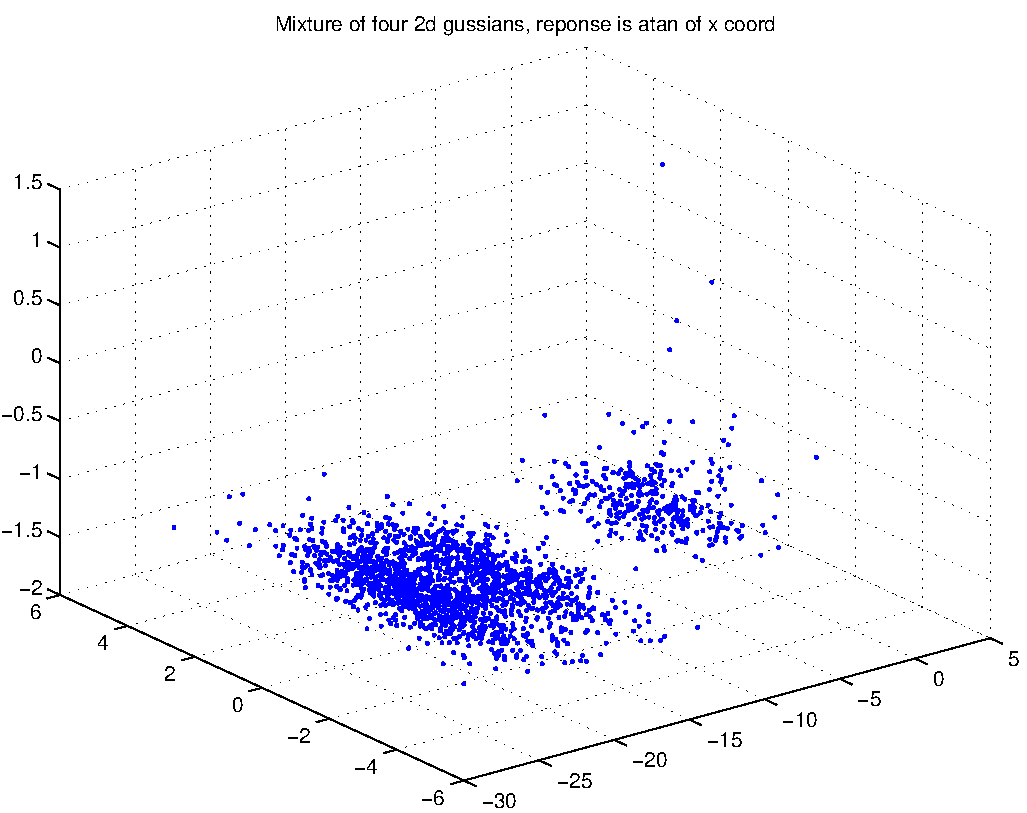
\includegraphics[width=10.0cm,height=10.0cm]{AtanDataSet.pdf}

\subsubsection{3 x 1 Linear Regression}
Sample size = 4000

Number of features = 3

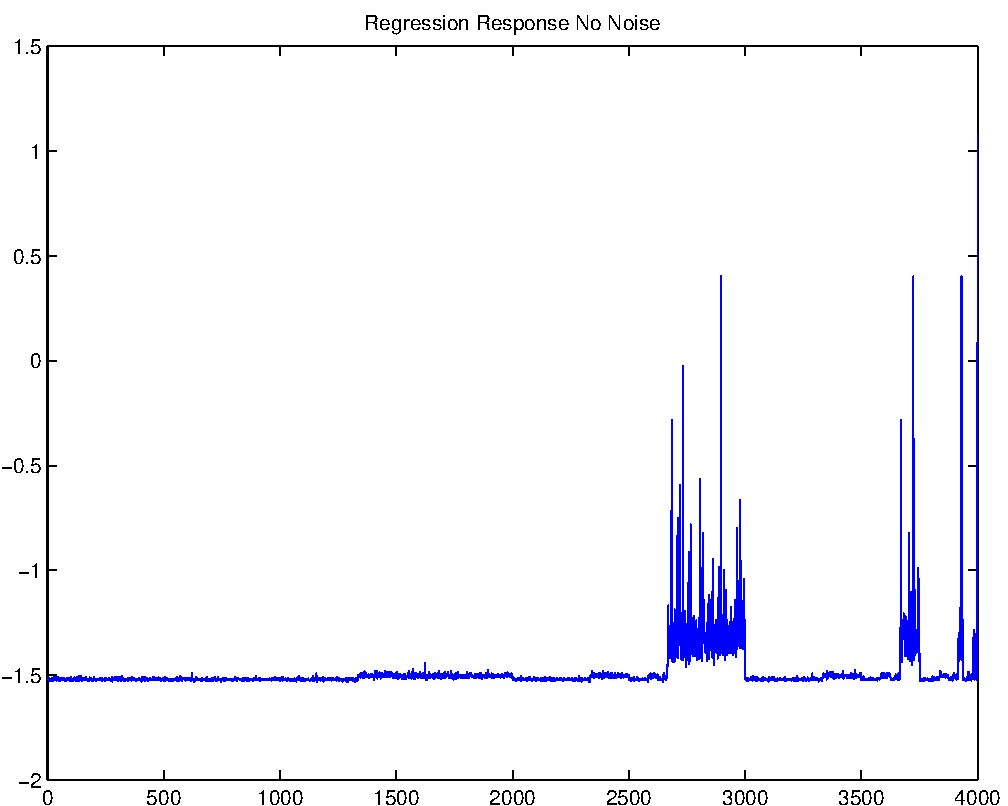
\includegraphics[width=10.0cm,height=10.0cm]{AtanDataSet_regression_response_no_noise.pdf}

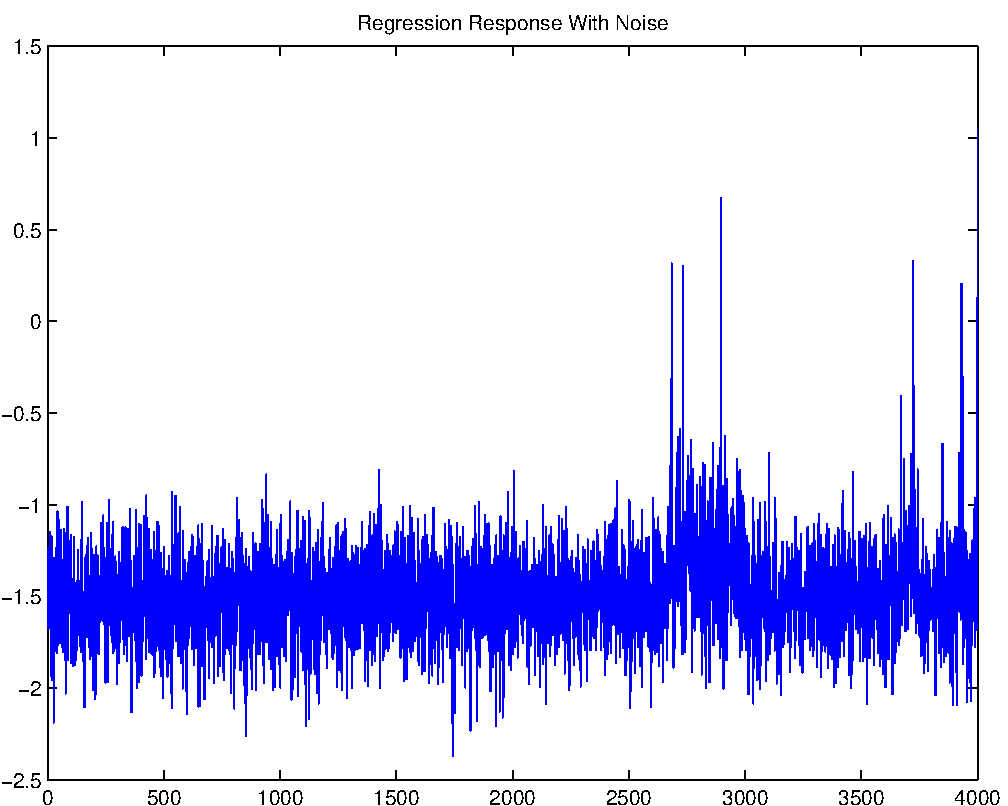
\includegraphics[width=10.0cm,height=10.0cm]{AtanDataSet_regression_response_with_noise.pdf}

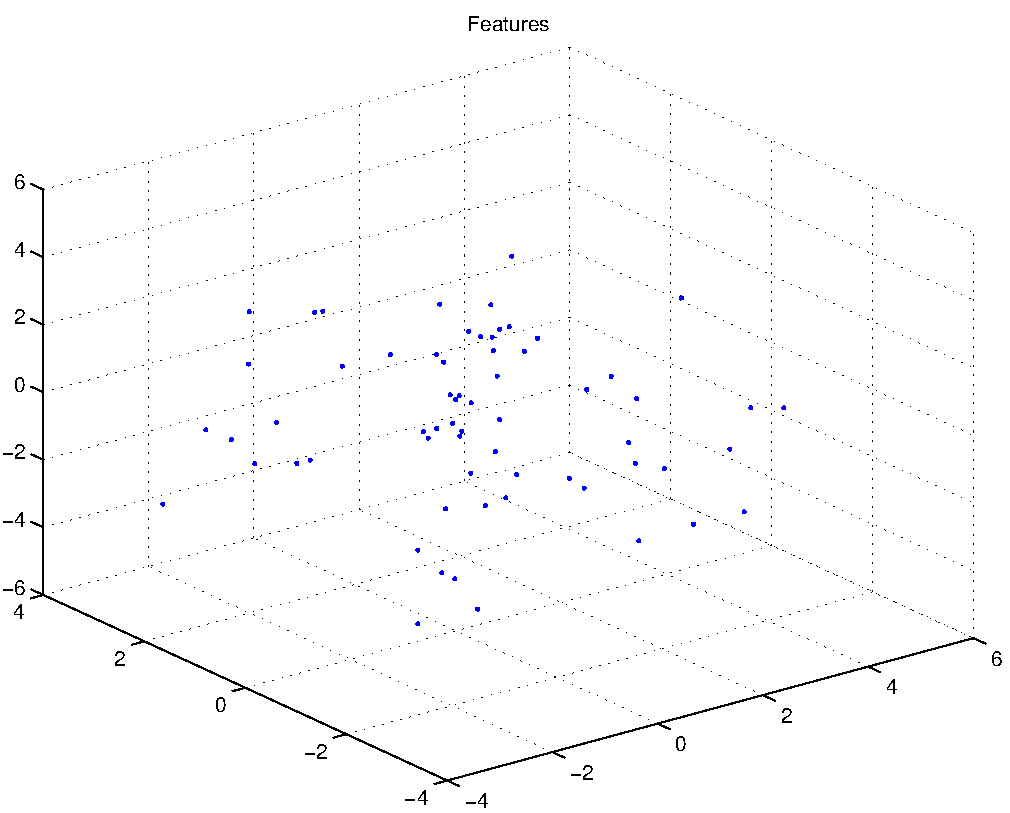
\includegraphics[width=10.0cm,height=10.0cm]{regression_features.pdf}

Response
-1.44217
-1.66486
-1.4752
1.41582
-1.31321
-1.3325
-1.21459
1.56204
-1.31651
-1.13275
-1.50392
1.43021
-1.7397
-1.4833
-1.13993
0.956543
-1.16884
-1.35312
-1.55636
1.31277
-1.42217
-1.51333
-0.946994
1.05129
-1.47725
-2.17262
-1.09945
1.4568
-1.45466
-1.75054
-1.29941
1.53827
-1.79685
-1.75661
-0.816739
1.7016
-1.26333
-1.48829
-1.17067
1.02668
-1.16778
-1.36854
-0.850966
1.57126
-1.22309
-1.74585
-0.951007
1.23368
-1.52506
-1.06793
-1.2426
1.53272
-1.55499
-1.73948
-1.15704
1.21939
-1.44857
-1.1086
-1.15193
1.2443
-1.49042
-1.75731
-1.30535
1.22384
-1.81293
-1.28966
-1.37758
0.98564
-1.53305
-1.47419
-0.88649
1.76224
-1.74061
-1.21536
-1.44356
1.02364
-1.60113
-1.99898
-0.703449
1.32517
-1.44012
-1.5133
-1.46497
1.81063
-1.3432
-0.991215
-1.33448
1.39595
-1.84897
-1.53994
-1.23875
1.50087
-1.38239
-1.50657
-1.11973
1.30231
-1.37504
-1.20111
-0.588045
1.05629
-1.81346
-1.48644
0.371557
1.12427
-1.69876
-1.81234
-1.14686
1.39036
-1.61449
-1.61563
-1.70528
1.37684
-1.17749
-1.35876
-1.55375
1.24605
-1.80999
-1.39688
-1.57239
1.34469
-1.66869
-1.60295
-1.54694
1.16392
-1.80327
-1.54002
-1.49627
1.40385
-1.40643
-1.21521
-1.17089
1.31304
-1.70204
-1.64967
-1.37072
1.31224
-1.5819
-1.76185
-1.59453
1.30203
-1.66625
-1.4447
-1.06155
1.09714
-1.79362
-1.16191
-1.37541
1.923
-1.63025
-1.7606
-1.67266
1.29993
-1.48718
-1.71679
-1.40825
1.16849
-1.67871
-1.47063
-1.91369
1.13971
-1.38352
-1.28327
-0.975642
1.46716
-1.68879
-1.58604
-1.2182
1.50667
-1.71523
-1.4817
-1.13153
1.39788
-1.38022
-1.18313
-1.0993
0.844635
-1.63746
-1.77217
-1.38058
1.29804
-1.49727
-1.58284
-1.72459
1.08174
-1.47834
-1.7994
-0.851979
1.67321
-1.5476
-1.41849
-1.02036
1.69753
-1.73104
-1.36635
-1.22654
1.45635
-1.99938
-1.37093
0.0068016
1.33013
-1.26722
-1.34103
-1.76832
1.14618
-1.34505
-1.38285
-1.71121
1.50104
-1.46515
-1.20654
-1.3543
1.56543
-1.6118
-1.71804
-1.05226
1.47216
-1.51693
-1.80309
-1.62149
1.16171
-1.81748
-1.42144
-1.45879
1.3063
-1.44904
-1.37977
-1.50454
1.22511
-1.54638
-1.09164
-1.35368
1.09977
-1.39511
-1.15752
-1.44375
1.20257
-1.51884
-1.42914
-1.27408
1.71115
-1.48281
-1.52172
-1.51013
1.14311
-1.32721
-1.72345
-1.08922
1.39369
-1.96228
-1.49281
-1.01734
1.49264
-1.43589
-1.35102
-0.954171
1.24161
-1.33686
-1.5662
-1.21568
0.77507
-1.95951
-1.45757
-0.718639
1.55895
-1.66482
-1.18163
-1.25365
1.50654
-1.56696
-1.61693
-1.30979
1.58296
-1.62685
-1.42187
-1.49012
1.41858
-1.19337
-1.72173
-0.936592
1.06624
-1.33895
-1.42916
-0.449622
1.13186
-1.64449
-1.58821
-1.56763
1.21256
-1.51178
-1.34143
-1.08161
1.07742
-1.43976
-1.29162
-1.39294
1.3119
-1.4194
-1.46575
-1.64696
0.930282
-1.35823
-1.39969
0.977817
1.4355
-1.68394
-1.60339
-1.14982
0.809855
-1.44126
-1.70014
0.678387
1.5258
-1.63516
-1.30473
-1.27163
1.31226
-1.5846
-1.49468
-1.20134
1.72797
-1.50251
-1.49724
-1.42198
1.49058
-1.11854
-1.56976
-1.33545
1.0658
-1.41964
-1.59758
-1.4738
1.32001
-1.42368
-1.55826
-1.03781
0.755334
-1.41675
-1.18687
-1.51839
1.59369
-1.42224
-1.16325
-1.67696
1.51268
-1.1302
-1.60052
-1.26681
1.20408
-1.41116
-1.42125
-1.57302
1.40891
-1.46579
-1.23557
-0.68531
1.81623
-1.60587
-1.47423
-1.39268
1.32426
-2.12596
-1.43116
-1.75618
1.32126
-1.45717
-1.66599
-1.30881
1.20066
-1.61109
-1.66482
-0.932605
1.40873
-1.5074
-1.66133
-0.710297
1.47839
-1.57856
-1.70576
-1.51191
1.87047
-1.85355
-1.34946
-1.68206
1.09986
-1.58716
-1.58946
-0.515816
1.21877
-1.25078
-1.35565
-1.26231
0.704414
-1.77354
-1.08769
-1.34281
1.62291
-1.61843
-1.8586
-1.42253
1.45759
-1.12131
-1.61517
-1.50123
0.171277
-1.67138
-1.52884
-1.41157
1.33909
-1.59536
-1.47632
-1.61199
1.32831
-1.5026
-1.43474
-1.43782
1.5259
-1.07445
-1.31991
-1.14627
1.2912
-1.50523
-1.82116
-1.43445
1.58888
-0.953615
-1.56607
-0.822323
1.1524
-1.26199
-1.42288
-1.22865
1.64549
-1.17107
-1.35568
-0.880596
1.31586
-1.79816
-1.66721
-1.15315
1.50805
-1.57065
-1.59011
-1.56686
1.38579
-1.25292
-1.38934
-1.69854
1.3832
-1.32768
-1.45127
-1.27834
1.35954
-1.83342
-1.62902
-1.3467
0.867481
-1.16522
-1.23774
-1.28415
-0.490836
-1.9027
-1.54597
-1.7998
0.925536
-1.24276
-1.72704
-1.5054
1.35734
-1.54189
-1.19273
-1.31862
0.963231
-1.09354
-1.157
-1.47599
1.0729
-1.38717
-1.09144
-1.15189
1.11771
-1.23283
-1.69957
-1.62081
1.55171
-1.72176
-1.50499
-1.21362
1.58287
-1.92577
-1.43986
-1.34707
1.35562
-1.49361
-1.50191
-1.10742
1.44388
-2.05581
-1.32892
-1.64263
1.19651
-1.22565
-1.26531
-1.54212
1.34378
-1.78922
-1.57702
-1.29483
0.998071
-1.84429
-1.3914
-1.2609
1.38211
-1.82584
-1.61472
-1.25258
0.75116
-1.774
-1.51419
-1.21435
1.38634
-1.27671
-1.78702
-1.30467
1.06937
-1.8647
-1.74641
-1.63058
1.40149
-1.36917
-1.45142
0.82852
0.941054
-1.39883
-1.46922
-0.647809
1.32581
-2.11754
-1.32665
-1.27626
1.48919
-1.43102
-1.29711
-1.31894
1.04527
-1.48767
-1.42408
-1.2468
1.47416
-1.47654
-0.955815
-1.25011
0.338039
-1.75429
-1.53261
-1.53428
1.17778
-1.62371
-1.37927
-1.27205
1.34816
-1.45873
-1.14755
-1.66237
1.25978
-1.72665
-1.43524
-1.19633
1.27979
-1.01557
-1.54525
-1.51279
1.18609
-1.87024
-1.65505
-1.25145
0.988229
-1.55061
-1.54138
-1.30571
1.27337
-2.00329
-1.33002
-0.973273
1.13303
-1.50338
-1.52091
-1.4161
1.48005
-1.30037
-1.44767
-1.06506
1.12401
-1.48037
-1.56175
-0.816077
1.55765
-1.85222
-2.1203
-1.67662
1.33018
-1.72291
-1.50511
-1.12607
1.15954
-1.75445
-1.28242
-0.831535
1.31185
-1.72981
-1.25183
-1.53959
1.03424
-1.40851
-1.41663
-1.41565
1.57434
-1.2203
-1.47503
-1.07692
1.13294
-1.18847
-1.27388
-1.07083
1.31341
-1.52236
-1.33178
-1.16477
1.31538
-1.31178
-1.83696
-1.35673
1.26586
-1.28756
-1.67029
-1.11394
1.52534
-1.47202
-1.7779
-1.39392
-0.230262
-1.77392
-1.25593
-1.00815
1.56326
-1.50699
-1.7202
-0.421418
1.83617
-2.09393
-1.25131
-1.22385
1.25975
-1.19189
-2.0844
-1.07122
1.24244
-1.4378
-1.564
-1.60999
0.754712
-1.44082
-1.69525
-1.23886
0.897518
-1.10413
-1.27334
-1.44211
1.58377
-1.31817
-1.6208
-1.57466
1.05141
-1.44996
-1.75136
-1.94699
1.10514
-1.8202
-1.82355
-1.56688
1.46184
-1.63075
-1.64585
-1.28506
1.53701
-1.45451
-1.38671
-0.426236
1.64259
-1.74272
-1.47566
-1.22476
1.447
-1.93321
-1.20859
-0.836064
1.26422
-1.4344
-1.71955
-1.58094
1.08811
-1.40379
-1.55165
-1.57671
1.20236
-1.42257
-1.3888
-1.31704
1.70344
-1.78581
-1.39974
-1.4866
1.21737
-1.71507
-1.36396
-1.43604
1.08802
-1.39876
-1.64636
-0.746155
1.21476
-1.5022
-1.30576
-1.14155
0.961492
-1.52178
-1.41017
-1.51093
0.902036
-1.2908
-1.54021
-1.02119
0.839325
-1.52625
-1.40795
-1.06947
1.35169
-1.53114
-1.58635
-1.51589
0.964867
-1.33046
-1.73563
-1.36504
1.3492
-1.27563
-1.56496
-1.37594
1.51312
-1.44855
-1.36999
-0.378322
1.39064
-1.43501
-1.89851
-1.10054
1.72709
-1.53155
-1.83686
-1.37217
0.808354
-1.33527
-1.63173
-1.3037
0.936135
-1.18766
-1.64096
-1.65933
1.20093
-1.53687
-1.63838
-0.982472
1.21635
-1.77518
-1.49628
-1.2829
1.22405
-1.73669
-1.40598
-1.40595
1.68839
-1.33038
-1.78812
-1.50073
1.08082
-1.8068
-1.48583
-1.26612
1.35593
-2.02977
-1.4696
-1.52892
0.956093
-1.64631
-1.69379
-1.06926
1.09637
-1.52818
-1.28324
-1.34272
0.8486
-1.41658
-1.78953
-1.92436
0.964428
-1.41786
-1.63861
-1.25605
0.82679
-1.18244
-1.17998
-1.10098
1.09195
-1.5849
-1.5639
-0.782978
1.34297
-1.33046
-1.36541
-1.0177
1.59885
-1.08677
-1.49938
-1.38452
1.38466
-1.47729
-1.316
-1.66728
1.22689
-1.56444
-1.8959
-1.41912
1.1492
-1.17398
-1.44636
-1.19996
1.39517
-1.14868
-1.28879
-1.21999
1.04338
-1.44324
-1.26002
-1.35894
1.25784
-1.98364
-1.30337
-1.22029
1.34876
-2.09007
-1.57538
-1.69112
1.49137
-1.62458
-1.57931
-2.09485
1.08245
-1.79923
-1.41135
-1.16305
1.1922
-1.53752
-1.74788
-1.66293
1.12062
-1.47944
-1.29142
-1.53061
1.5403
-1.66024
-1.82012
-1.42983
1.19916
-1.68114
-1.35422
-1.53157
0.879021
-1.67741
-1.47469
-0.68148
1.39893
-2.00719
-1.1349
-1.36474
1.02733
-1.34696
-1.39827
-1.43514
1.17151
-1.649
-1.30248
-1.30258
1.58089
-1.57484
-1.20111
-1.90485
1.21507
-1.46697
-1.21145
-1.57368
1.39112
-1.80245
-1.61611
-1.04465
1.59549
-1.80774
-1.76893
-0.851332
1.30818
-1.60589
-1.37579
-1.66256
1.00144
-1.2928
-1.19712
-1.60477
1.37452
-1.54655
-1.47821
-1.57722
1.10037
-1.39975
-0.970392
-1.51554
1.23476
-1.58043
-1.43838
-0.93288
0.740783
-1.87868
-1.69692
-1.77029
1.06619
-1.75167
-1.58277
-1.08969
1.39354
-1.09474
-1.3838
-1.10095
1.17706
-0.832665
-1.72884
-1.1796
1.4321
-1.55766
-1.53473
-0.843292
1.25773
-1.50957
-1.43084
-1.24132
1.41791
-1.3939
-1.20897
-0.885992
1.63398
-1.83342
-1.67386
-1.35562
1.1322
-1.90743
-1.08936
-1.54477
-0.435308
-1.68459
-1.32212
-1.66119
1.40158
-1.68708
-1.38262
-1.85202
0.991704
-1.59238
-1.70985
-1.19417
0.893912
-1.56062
-1.64427
-1.13774
1.351
-1.28058
-1.43816
-1.41566
1.27263
-1.13849
-1.25045
-1.61973
1.27055
-1.49081
-1.44301
-1.37087
0.804271
-1.34621
-1.37619
-1.62082
1.52263
-1.59911
-1.18234
-0.902419
1.28202
-2.00013
-1.65723
-0.900383
1.05875
-1.61437
-1.59602
-1.14292
1.35834
-1.78273
-1.3288
-1.47249
1.20016
-1.34336
-1.44401
-0.294668
1.63314
-1.81874
-1.43532
-1.12572
1.60346
-1.29162
-1.66323
-1.02952
1.44727
-1.55702
-1.54729
-1.71431
1.50491
-1.54355
-1.44951
-1.3383
1.37163
-1.3992
-1.58021
-0.982917
1.2652
-1.25975
-1.45531
-1.14431
1.08038
-1.52462
-1.47864
-1.51071
0.518083
-1.57997
-1.51988
-1.49126
1.33921
-2.0567
-1.5833
-1.64579
1.54236
-1.44318
-1.98199
-1.44321
1.23768
-1.72998
-1.41492
-1.41532
1.22187
-1.37844
-1.39471
-1.30448
1.2269
-1.93802
-1.3201
-1.11476
1.17431
-1.39385
-1.25393
-1.03867
1.70063
-1.70894
-1.38402
-0.950438
0.444989
-1.83612
-1.50565
-1.15471
1.37913
-1.50401
-1.65288
-1.16591
0.792233
-1.6135
-1.63407
-1.43419
1.43372
-1.38191
-1.43256
-0.76033
1.1154
-1.49686
-1.43523
-1.41499
1.49336
-1.28111
-1.33339
-1.38066
1.85014
-1.90284
-1.3372
-1.19956
0.946012
-1.0827
-1.77524
-1.22387
0.80522
-1.52801
-1.29787
-1.87831
1.15113
-1.54273
-1.48789
-1.5796
1.5151
-1.33135
-1.88441
-1.42683
0.941475
-1.54797
-1.28244
-1.48486
0.687215
-1.02068
-1.5483
-0.377414
1.41492
-1.78322
-1.56103
-0.86543
1.32629
-1.49354
-1.86402
-1.23666
1.23886
-1.41372
-1.54847
-1.39063
1.1039
-1.37352
-1.2069
-1.05024
1.39652
-1.66148
-1.24748
-1.36123
0.885765
-1.39135
-1.474
-1.64136
1.37226
-1.35377
-1.79685
-1.03006
1.19852
-1.65435
-1.29981
-1.09803
0.755398
-1.76908
-1.11835
-1.58657
0.840665
-1.74892
-2.06716
-1.66675
1.52704
-1.59793
-1.54871
-1.18405
0.925617
-1.47469
-1.34255
-1.47422
1.38407
-1.18492
-1.5857
-1.09369
1.40197
-1.59857
-1.20982
-0.78126
1.30715
-1.3424
-1.42034
-1.46391
0.924936
-1.53254
-1.26516
-1.02397
1.45876
-1.63444
-1.59875
-1.44708
1.28189
-1.72857
-1.69482
-1.07475
1.04305
-1.36825
-1.46749
-1.52675
1.36496
-1.45357
-1.51273
-1.28103
1.29831
-1.51285
-1.45559
-1.33401
1.57624
-1.18116
-1.33325
-1.13973
1.48705
-1.61502
-1.33606
-1.35568
1.01493
-1.65171
-1.8035
-0.964577
1.34029
-1.76584
-1.68917
-0.78044
1.07269
-1.28378
-1.36681
-1.49751
1.38665
-1.46737
-1.46101
-1.63217
-0.574794
-1.51961
-1.3378
-1.05906
1.12122
-1.18104
-1.29768
-1.03125
1.01972
-2.00124
-1.3872
-1.20127
1.79847
-1.54726
-1.46733
-1.63939
0.878198
-1.62687
-1.59829
-1.41344
1.53642
-1.26101
-1.65786
-1.12174
0.850555
-1.67288
-1.15752
-1.47072
0.957298
-2.01338
-1.49672
-1.05194
1.49162
-1.46165
-1.44336
-0.968255
1.21754
-1.65106
-1.61046
-0.673177
1.33814
-1.60022
-1.64449
-1.38273
0.96816
-1.08352
-1.7182
-1.26817
1.68462
-1.32192
-1.68643
-1.22929
0.866093
-1.49398
-1.33825
-1.55404
1.55261
-1.38984
-1.53253
-1.50826
1.28704
-1.56659
-1.70616
-1.25832
0.931748
-1.53477
-1.29938
-1.47068
1.2976
-1.61208
-1.62339
-1.55291
1.64637
-2.00496
-1.59524
-1.16784
1.15323
-1.50706
-1.25048
-1.20257
1.60226
-1.46143
-1.80328
-1.27367
1.01296
-1.72498
-1.27875
-1.09542
1.03392
-1.75261
-1.21133
-1.29977
1.16464
-1.67974
-1.67361
-1.41605
1.16209
-1.78407
-1.22931
-1.61046
1.03458
-1.5696
-1.46807
-1.06258
1.51402
-1.66815
-1.53022
-1.42217
1.08477
-1.44422
-1.31613
-1.2405
1.23068
-1.27452
-1.23404
-1.34023
1.68671
-1.65649
-1.39253
-1.50593
1.38652
-1.39294
-1.30025
-1.19506
1.52963
-1.53051
-1.67583
-1.1472
0.998101
-1.97377
-1.24353
-1.64378
1.16334
-1.54608
-1.60649
-1.64137
1.3986
-1.54035
-1.21236
-0.930725
1.54958
-2.01044
-1.69781
-1.30906
1.18465
-1.64259
-1.08574
-0.830248
1.6137
-1.54882
-1.32297
-1.07798
1.87525
-1.19495
-1.18913
-1.56457
1.00063
-1.56444
-1.31791
-1.57822
1.55215
-1.35649
-1.6326
-1.0683
0.866057
-1.21828
-1.41825
-1.3464
1.27135
-1.07064
-1.80939
-1.71576
1.56925
-1.69309
-1.38068
-0.927775
1.34442
-1.38347
-1.12551
-1.485
1.02472
-1.75278
-1.1577
-1.3382
1.29414
-1.38163
-1.45987
-1.16946
1.96966
-1.33941
-1.56998
-1.59134
0.364531
-1.73966
-1.22438
-1.8285
1.33314
-1.00786
-1.35992
-1.29673
1.3672
-1.71209
-1.54066
-1.09457
1.11564
-1.38436
-1.85287
-1.24603
1.43242
-1.46629
-1.49721
-1.74879
1.12574
-1.77127
-1.72004
-1.19095
1.09445
-1.28621
-1.59186
-1.17418
1.44958
-1.6529
-1.79004
-1.35877
1.58304
-1.72717
-1.5184
-1.08514
0.96559
-1.4832
-1.43511
-1.4721
1.04477
-1.34067
-1.30668
-1.43414
1.59184
-1.645
-1.69416
-1.40281
1.53469
-1.4634
-1.64481
-1.12385
1.28828
-1.31333
-1.28332
-1.40741
1.32454
-1.77009
-1.41493
-1.07563
1.65652
-1.5256
-1.486
-1.12698
1.26952
-1.17063
-1.3596
-1.59134
0.56743
-1.29714
-1.54949
-1.44497
1.08936
-1.42223
-1.08059
-1.1304
1.72914
-1.23638
-1.57882
-0.132718
1.39054
-1.70672
-1.2729
-1.27329
1.12823
-1.63981
-1.53082
-1.23611
1.31227
-1.5528
-1.81721
-1.17818
1.40109
-1.1505
-1.34119
-0.256868
1.2757
-1.65428
-1.57912
-0.893692
1.89463
-1.43301
-1.49556
-1.55004
1.41187
-1.9749
-1.35874
-1.13383
1.0108
-1.56796
-1.17878
-1.41877
1.16258
-1.32717
-1.55113
-1.26906
0.846603
-1.3892
-1.62091
-1.42189
1.17494
-1.78795
-1.34928
-1.06729
1.09335
-1.19092
-1.41403
-0.820025
1.47923
-1.81534
-1.00767
-1.61143
1.31666
-1.59368
-1.58807
-1.60639
1.10438
-1.11897
-1.28175
-1.16997
1.72239
-1.41745
-1.46224
-1.04214
1.46429
-1.58621
-1.63451
-1.45361
1.66586
-1.34375
-1.28975
-1.29509
1.22083
-1.75912
-1.68914
-1.29404
1.34237
-1.67816
-1.67084
-0.713905
1.38028
-1.44776
-1.47853
-1.38545
1.45631
-1.85698
-1.08132
-1.18294
1.04263
-1.63109
-1.25655
-1.79401
1.10317
-1.73005
-1.3821
-1.47102
1.22402
-1.34176
-1.55918
-1.61863
0.852218
-1.27681
-1.92313
-0.830053
1.50744
-1.59561
-1.46692
-1.5724
1.06923
-1.18074
-1.47083
-1.26688
1.59614
-1.91718
-1.11586
-1.22055
1.24306
-1.64789
-1.46632
-1.59878
0.933013
-1.5884
-1.48723
-1.01925
1.31713
-1.52127
-1.21054
-1.48332
1.44927
-1.36964
-1.34617
-1.16768
1.28258
-1.98681
-1.742
-1.28161
1.39412
-1.46061
-1.64415
-1.49961
1.01545
-1.54367
-1.60095
-1.27587
1.50677
-1.62615
-1.42446
-1.75477
1.2779
-1.80744
-1.60523
-1.61378
1.68743
-1.39862
-1.39344
-1.53291
1.45298
-1.68964
-1.86909
-1.01039
1.14883
-1.75955
-1.28142
-1.62728
0.695908
-1.2951
-1.59941
-1.14659
1.59366
-1.50931
-1.65394
-1.32596
0.811394
-1.64436
-1.3201
-1.3418
0.907831
-1.75316
-1.48228
-1.20732
1.62172
-1.61072
-1.34357
-1.12804
1.17704
-1.6976
-1.26102
-1.01992
1.10165
-1.71599
-1.75791
-1.29237
0.945378
-1.45636
-1.52607
-1.41235
1.45314
-1.71636
-1.63106
-1.49405
1.24955
-1.13314
-1.36623
-1.30897
1.27848
-1.50103
-1.23202
-1.54162
1.49711
-1.59736
-1.24545
-1.54596
1.51274
-1.29295
-1.34235
-1.1177
1.57274
-1.6961
-1.15971
-0.25285
1.84512
-1.57898
-1.30333
-1.06953
0.957395
-1.70356
-1.66507
-0.90097
1.27527
-1.4647
-1.64779
-1.49303
0.700836
-1.97336
-2.38458
-1.20082
1.27925
-1.80471
-2.01158
-1.57785
1.01515
-1.56331
-1.73656
-1.47472
1.12412
-2.14891
-2.01547
-1.20642
1.50016
-1.56375
-1.4865
-1.11899
1.10334
-1.41263
-1.11179
-1.47564
1.3779
-1.72975
-1.7532
-1.5237
0.950206
-1.38539
-1.64008
-1.41574
1.03629
-1.18825
-1.185
-1.12326
1.49131
-1.65202
-1.55363
-0.118801
1.49771
-1.87111
-1.60917
-1.66308
1.42361
-1.22498
-1.11752
-1.23344
1.39941
-1.53251
-1.43487
-1.02755
1.38591
-1.38847
-1.45395
-1.26677
1.44279
-2.00709
-1.31296
-1.51597
1.26474
-1.68923
-1.49151
-1.46228
1.13373
-1.82738
-1.2352
-0.900189
1.44212
-1.38217
-1.77425
-0.820854
1.39012
-1.45136
-1.64274
-1.49636
1.53679
-1.65681
-1.88034
-2.11168
1.32381
-1.57714
-1.35552
-1.38001
1.63417
-1.36238
-1.67097
-1.23971
1.46784
-1.67867
-1.19409
-1.31183
1.49159
-1.67972
-1.62481
-1.36568
1.25958
-1.72744
-1.00462
-1.56403
1.05193
-1.28504
-1.1642
-1.31136
1.04289
-1.69994
-1.71746
-1.45517
0.579042
-1.35838
-1.32774
-1.67149
1.10958
-1.50923
-1.42285
-1.50749
1.09385
-1.87464
-1.5206
-0.867884
1.45589
-1.8995
-1.73023
-1.04429
1.65343
-1.56612
-1.4157
-1.34176
1.1305
-1.30203
-1.44312
-1.67023
0.600759
-1.37103
-1.24882
-1.16911
1.49701
-1.52385
-1.46566
-1.17053
1.73536
-1.59813
-1.43613
-1.43434
1.67193
-1.53384
-1.34714
-1.24402
1.34988
-1.50064
-1.09165
-0.840276
1.25245
-1.46571
-1.72586
-0.968654
1.43336
-1.11493
-1.80987
-1.3531
1.58871
-1.24006
-1.72984
-1.58955
1.0295
-2.02169
-1.56231
-0.854779
1.5069
-1.63975
-1.34053
-1.27518
0.975895
-1.38809
-1.63978
-1.65981
1.44026
-1.63441
-1.65836
-1.33836
1.58751
-1.35789
-1.68513
-1.15537
1.62373
-1.40004
-1.70181
-1.72538
1.25806
-2.23095
-1.172
-1.51889
1.12208
-1.73113
-1.39274
-1.3805
1.1989
-1.3741
-1.27481
-1.38992
1.43546
-1.70626
-1.62078
-1.47709
1.33595
-2.15272
-1.47078
-1.25057
1.61631
-1.33375
-1.26043
-1.00895
1.72524
-1.4035
-1.62453
-1.28374
1.28137
-2.19073
-1.84178
-1.57698
0.673667
-1.28611
-1.15501
-1.82159
1.23656
-1.25966
-1.72922
-1.63305
0.60946
-1.27811
-1.3016
-0.828338
1.48132
-1.51324
-1.30079
-0.755792
1.39836
-1.68726
-1.38655
-1.3303
1.39108
-0.962357
-1.60237
-1.17381
0.975675
-1.43777
-1.73452
-1.74658
1.01114
-1.50812
-1.4061
-1.19227
0.900003
-1.31859
-1.31727
-1.19447
1.7381
-1.47372
-1.45307
-1.07522
0.999181
-1.27682
-1.77215
0.0127115
1.39282
-0.811209
-1.48526
-0.48518
1.3786
-1.77047
-1.35854
-1.31734
1.18854
-1.14634
-1.3205
-1.18958
1.45197
-1.73344
-1.31267
-0.89763
1.22932
-1.66844
-1.8299
-1.31488
1.11217
-1.55364
-1.48571
-1.4487
1.07213
-1.2893
-1.57118
-1.1374
1.67643
-1.57445
-1.41066
-0.850333
1.40003
-1.55989
-1.64262
-1.2561
1.29811
-1.45766
-1.7098
-1.48473
1.09953
-1.75098
-1.27232
-0.908768
1.38429
-1.43669
-1.44156
-1.45923
1.39431
-1.31182
-1.5894
-1.28921
1.24274
-1.44639
-1.59168
-1.28551
1.66207
-1.70776
-1.07343
-1.30762
0.738465
-1.43112
-1.73059
-1.55311
1.02539
-1.50399
-1.36203
-1.3609
0.857595
-1.43899
-1.77958
-1.63327
0.667768
-1.53474
-1.34224
-1.40147
1.36575
-1.55263
-1.34597
-1.18867
1.18288
-1.51325
-1.55844
-1.49408
1.43496
-1.40682
-1.42257
-1.16409
1.69062
-1.30509
-1.2543
-1.19477
0.84275
-1.78191
-1.79003
-1.187
1.3491
-1.37407
-1.59702
-1.23531
0.986188
-1.36974
-1.68134
-1.45043
1.13191
-1.4931
-1.79318
-0.725245
1.69768
-1.6324
-1.66693
-1.3491
1.00085
-1.99987
-1.29139
-1.47999
1.51338
-1.58708
-1.41692
-1.63706
1.18004
-1.28617
-1.64152
-1.21053
1.19189
-1.30695
-1.85301
-0.789732
1.38174
-1.32241
-1.44726
-1.10676
1.63971
-1.46904
-1.48525
-1.18159
1.01313
-1.65066
-1.52049
-0.968802
0.692387
-1.69261
-1.41567
-1.4136
1.09465
-1.67779
-1.39865
-1.51091
1.23346
-1.44934
-1.46559
-1.27506
-0.505066
-1.40163
-1.47825
-1.00274
1.35554
-1.53357
-1.80322
-1.24533
1.68299
-1.76092
-1.10081
-1.14779
1.03527
-1.66952
-1.34442
-0.930424
1.58371
-1.21561
-1.642
-1.47007
1.59798
-1.51767
-1.41628
-1.44478
1.35705
-1.87456
-1.56646
-1.23621
1.13525
-1.39682
-1.54444
-1.4553
1.04614
-1.47231
-1.4811
-1.47566
1.16596
-1.79943
-1.62935
-0.105253
1.39366
-1.19245
-1.76948
-1.16962
1.62874
-1.75995
-1.45742
-1.64606
-0.378954
-1.42239
-1.38468
-1.27719
1.15399
-1.56441
-1.53713
-1.00294
1.26901
-1.21801
-1.05349
-1.35742
1.33245
-1.49849
-1.7308
-1.4833
1.34318
-1.36731
-1.67776
-1.0148
0.810573
-1.72258
-1.59642
-1.2495
1.38698
-1.42392
-1.00351
-1.47815
1.47575
-1.64828
-1.44598
-0.943019
1.08544
-1.67549
-1.77305
-1.10448
1.22348
-2.00157
-1.64841
-1.02389
1.5617
-1.33489
-1.96292
-1.0935
1.5547
-1.2974
-1.29442
-1.00533
1.38234
-1.5273
-1.4517
-1.054
1.53753
-1.63736
-1.35324
-1.25829
0.874742
-1.63373
-1.71717
-1.59091
0.723689
-1.46676
-1.7226
-1.34412
1.54074
-1.54699
-1.51611
-1.10811
1.29004
-1.64804
-1.70025
-1.38921
1.50126
-1.50314
-1.40269
-1.41959
1.26027
-1.72234
-1.7427
-1.55919
1.02316
-1.63482
-1.30034
-1.24249
1.30386
-1.90269
-1.35485
-1.41112
1.07451
-1.98717
-1.39845
-1.15427
1.38727
-1.53943
-1.47459
-1.21923
1.39675
-1.44135
-1.51239
-1.07116
1.65093
-1.24443
-1.23566
-1.48395
1.63843
-1.48472
-1.37651
-1.61436
1.58934
-1.34224
-1.74913
-1.42112
1.10235
-1.514
-1.29747
-1.01996
1.46742
-1.47053
-1.92908
-0.234231
1.40423
-1.51746
-1.36358
-1.27625
1.37626
-1.43123
-1.43564
-1.39381
1.21819
-1.40351
-1.40859
-1.50302
1.10226
-1.49921
-1.25291
-1.22866
1.12776
-1.48348
-1.6864
-1.24318
1.39628
-1.5947
-1.69969
-1.12373
1.68991
-1.31335
-1.71722
-1.07375
1.54967
-1.69165
-1.54012
-1.29501
1.30981
-1.54953
-1.38478
-1.54439
1.21097
-1.70112
-1.15822
-1.28157
1.47819
-1.38859
-1.57845
-1.00447
1.55186
-1.51851
-1.26658
-0.817606
1.57877
-1.4971
-1.52371
-1.13768
1.2108
-1.43878
-1.38741
-1.74019
0.842132
-1.3428
-1.46516
-0.581597
1.51494
-1.38665
-1.50684
-1.49362
0.810353
-1.57634
-1.40813
-1.21644
1.3495
-1.79161
-1.52636
-1.43116
1.55015
-1.2932
-1.5367
-1.73206
1.16552
-1.42226
-1.54042
-1.19707
1.55475
-1.60905
-1.45694
-1.10169
0.785331
-1.31094
-1.65445
-1.68936
1.6109
-1.33869
-1.11552
-1.17447
1.57126
-1.34689
-1.73743
-1.20242
1.14656
-1.45629
-1.11842
-1.48318
0.970944
-1.48461
-1.49838
-1.15599
1.31471
-1.45924
-1.64737
-0.901594
1.33373
-1.48504
-1.08346
-1.34211
1.52652
-1.41027
-1.54949
-1.22344
1.13611
-1.49462
-1.63508
-0.873886
0.91425
-1.57972
-1.68668
-1.20211
1.9212
-1.28559
-1.55688
-1.0381
1.56403
-1.72075
-1.60579
-1.64405
0.887843
-1.46741
-1.34323
-1.54458
1.33651
-1.52668
-1.81675
-1.12089
1.35865
-1.71601
-1.6625
-1.18082
1.17408
-1.29104
-1.62432
-1.02939
1.23215
-1.43925
-1.43991
-1.57694
1.26042
-1.56905
-1.21315
-1.19591
1.4084
-1.60388
-1.4558
-1.5479
1.07816
-1.25967
-1.91655
-1.10127
1.40014
-1.55821
-1.84954
-1.5176
1.05996
-1.67448
-1.41436
-1.48381
1.32561
-1.72566
-1.53414
-1.10232
1.049
-0.962462
-1.67061
-0.73844
0.838672
-1.56624
-0.970926
-1.26128
1.4276
-1.71343
-1.67972
-1.82385
1.63555
-1.70134
-1.84772
-1.64774
0.935336
-1.08223
-1.24853
-0.932095
1.25626
-1.72296
-1.70839
-1.10052
1.43846
-1.62456
-1.7924
-1.66
1.17853
-1.46973
-1.45564
-1.0582
1.36994
-1.43724
-1.64236
-1.32961
1.69154
-1.29879
-1.19193
-1.4845
0.246
-1.32034
-1.30936
-1.30316
1.42575
-1.55003
-1.66132
-1.23728
1.23208
-1.25011
-1.86824
-1.05007
1.52569
-1.55428
-1.45064
-1.77875
0.859915
-1.02718
-1.06873
-1.46097
1.34567
-1.61921
-1.56582
-1.28286
0.707811
-1.26303
-1.31104
-1.16062
1.38351
-1.68403
-1.30272
-1.45497
1.27865
-1.30323
-1.26061
-1.40777
1.70857
-1.38423
-1.21203
-1.25646
1.67832
-1.46674
-1.41539
-1.48643
1.00463
-1.66074
-1.43722
-0.915194
1.74902
-1.48857
-1.43317
-1.51348
1.10652
-1.8285
-1.69104
-1.91335
1.41968
-1.66295
-1.85839
-1.39673
1.15283
-1.67989
-1.6524
-1.25974
1.35695
-0.975816
-1.78666
-1.46879
1.10242
-1.10342
-1.77406
-1.14969
1.25021
-1.83237
-1.48624
-1.36405
1.55661
-1.28202
-1.14199
-1.44453
1.35136
-1.8141
-1.6521
-1.03964
1.5056
-1.46852
-1.18207
-0.891333
1.58913
-1.8847
-1.44958
-1.16807
1.4534
-1.25506
-1.69755
-1.57723
1.62086
-1.49066
-1.35978
-1.44939
1.65471
-1.43869
-1.49616
-1.02595
1.14016
-1.25204
-1.93944
-1.20626
1.41689
-1.40459
-1.44037
-1.42829
1.22655
-1.57694
-1.66973
-1.14491
1.41706
-1.45021
-1.3106
-1.25862
1.31005
-1.39877
-1.4719
-1.70628
1.24257
-1.1726
-1.5179
-1.12315
1.65295
-1.81572
-1.58863
-1.41311
1.45832
-1.6162
-1.6058
-1.45521
1.57811
-1.21326
-1.58639
-1.41126
1.66503
-1.1739
-1.68766
-1.22836
1.88238
-1.56798
-1.68707
-0.731403
1.45435
-1.67109
-1.76206
-1.32815
0.93963
-1.43099
-1.95133
-1.13089
1.05573
-1.63098
-1.59596
-1.65868
1.45373
-1.72801
-1.74567
-1.25621
1.71828
-1.61057
-1.83352
-1.39159
0.743713
-1.41128
-1.39079
-1.37174
0.905334
-1.65274
-1.67436
-1.41215
1.61414
-1.14008
-1.05612
-1.19995
1.55696
-1.51694
-1.21028
-1.30928
0.919681
-1.41228
-1.56384
-1.21586
1.28908
-1.53928
-1.58337
-1.78638
1.49504
-1.74828
-1.18576
-1.45932
0.779814
-1.51201
-1.34919
-1.06414
1.41848
-1.44034
-1.35191
-1.72418
1.2713
-1.56842
-1.78689
-1.45832
1.10625
-1.36072
-1.19991
-1.08947
1.84083
-1.46474
-1.62245
-1.04422
1.66973
-0.988571
-1.37079
-1.12896
1.41956
-1.56759
-1.5226
-1.1361
1.25779
-1.54937
-1.35862
-1.21488
1.29326
-1.41453
-1.90723
-1.89573
1.11119
-1.62728
-1.36077
-0.899213
1.25676
-1.59612
-1.27074
-1.60243
1.13609
-1.69028
-1.78074
-1.63683
1.30661
-1.36979
-1.283
-1.05279
1.48637
-1.6985
-1.4513
-1.36682
1.18158
-1.70522
-1.11699
-1.49174
1.36552
-1.71984
-1.44787
-1.31368
1.54656
-1.46773
-1.72353
-1.23421
1.04575
-1.79372
-1.51407
-0.521074
1.49223
-1.10715
-1.50419
-1.32958
1.3892
-2.01842
-1.35464
-1.45685
0.886671
-1.76856
-1.93665
-1.17783
1.43026
-1.46373
-1.31318
-1.17065
1.22073
-1.73721
-0.928697
-1.15942
0.828801
-1.47615
-1.41313
-1.12948
0.744129
-1.83331
-1.53262
-1.40492
1.16909
-1.55718
-1.35413
-1.08901
1.26544
-1.26911
-1.62157
-0.148072
1.52016
-1.84754
-1.21419
-1.86639
1.58981
-1.22588
-1.73233
-1.34424
1.47685
-1.68096
-1.4192
0.0483126
1.26059
-1.60391
-1.07204
-1.22356
1.56865
-1.59056
-1.22299
-0.885458
0.986462
-1.30649
-1.22405
-1.56191
1.13421
-1.73417
-1.59654
-1.68696
1.19577
-1.67199
-1.30291
-1.41946
0.950077
-1.79795
-1.1299
-1.20222
1.15245
-1.07936
-1.61446
-1.16457
1.89981
-1.34845
-1.29059
-1.28677
1.63143
-1.36519
-1.84022
-1.70305
0.677721
-1.20262
-1.47201
-1.4837
1.60062
-1.56658
-1.42481
-1.38416
1.43477
-2.00536
-1.33154
-1.01489
1.32614
-1.44755
-1.67276
-2.03115
0.521527
-2.04585
-1.43361
-1.27081
2.11324
-1.61386
-1.16808
-1.40199
1.40337
-1.54321
-1.62546
-0.871596
0.949834
-1.73254
-1.66368
-0.941832
1.38488
-1.19423
-1.54584
-1.50552
1.5281
-1.66448
-1.36586
-1.31623
1.19242
-1.62876
-1.34175
-1.29642
1.32484
-1.49538
-1.67151
-1.18106
0.775442
-1.2838
-1.49414
-1.19963
1.15046
-1.27661
-1.5575
-1.09228
1.71167
-1.0964
-1.35206
-1.11347
1.315
-1.71211
-1.47396
-1.19245
1.37148
-1.49912
-1.75882
-1.03551
1.59975
-1.43893
-1.26521
-1.55813
1.32139
-0.938641
-1.57609
-1.445
1.2274
-1.4793
-1.15312
-0.902646
1.49554
-1.64342
-1.79349
-1.25052
1.60164
-1.98447
-1.69241
-1.47348
1.37461
-1.63165
-1.64403
-1.39452
1.23092
-1.75264
-1.7805
-1.23201
0.740765
-1.86917
-1.09563
-1.61124
0.226819
-1.60939
-1.33829
-1.5782
1.31508
-1.22801
-1.39215
-1.30238
1.43772
-1.45656
-1.71885
-1.35478
1.55187
-1.79501
-1.28809
-1.06637
1.25491
-1.65195
-1.55846
-0.98491
1.61072
-1.39684
-1.72237
-1.38896
1.30466
-1.61373
-1.19934
-1.32157
1.37308
-1.50623
-1.81388
-1.54908
1.40815
-1.6084
-1.71287
-1.43884
1.24449
-1.4704
-1.26756
-1.31336
1.5738
-1.92921
-1.61815
-0.541177
0.830596
-1.56691
-1.54383
-0.856897
0.985024
-1.61419
-1.75747
-1.15086
1.56207
-1.58656
-1.57674
-1.62202
1.0661
-1.50779
-1.73461
-0.431735
0.992339
-1.55395
-1.55544
-0.750557
1.00607
-1.95599
-1.78478
-1.45113
1.62574
-1.80991
-1.54497
-1.04876
1.79757
-2.00276
-1.40295
-1.71208
1.5007
-1.50732
-1.52823
-1.07552
1.24546
-1.60091
-1.36821
-1.42571
1.44042
-1.27427
-1.53707
-0.988244
1.55567
-1.35747
-1.47472
-1.43948
1.23491
-1.65863
-0.967656
-1.29142
1.15767
-1.96372
-1.19209
-0.94258
1.27738
-1.56974
-1.24574
-1.04361
1.27995
-1.50581
-1.33372
-1.0439
0.986739
-1.80171
-1.52086
-0.640331
0.470303
-1.78705
-1.40721
-1.3442
1.5859
-1.81007
-1.56831
-0.863094
1.20706
-1.52847
-1.54052
-1.42223
1.20855
-1.64815
-1.68367
-1.42614
1.2751
-1.20766
-1.38885
-1.34619
1.4594
-1.5797
-1.3698
-1.69995
0.96164
-1.3957
-0.946042
-1.29736
1.38931
-1.24806
-1.07301
-1.5227
0.726403
-1.51406
-1.50173
-1.29412
1.23191
-1.74004
-1.71298
-1.38579
0.979577
-1.44957
-1.3977
-1.19424
0.906931
-1.53113
-1.54257
-1.3683
1.32358
-1.5233
-2.02036
-1.17174
1.20658
-1.6438
-1.63354
-1.42902
1.31261
-1.18992
-1.38528
-0.91711
1.42159
-1.57966
-1.74819
-1.51178
1.18113
-1.58944
-1.54843
-1.27959
1.22683
-1.67966
-1.42047
-1.22244
1.43002
-1.52713
-1.51758
-1.38943
1.57797
-1.40288
-1.19352
-1.4044
1.0031
-1.22374
-1.67312
0.784233
1.39857
-1.60118
-1.2548
-1.55175
1.39471
-1.91199
-1.87208
-1.46288
1.4492
-1.7743
-1.75195
-1.30632
1.47761
-1.25489
-1.38674
-1.15552
1.26625
-1.32372
-1.41041
-1.01369
1.34509
-1.50423
-1.6067
-1.31831
1.03821
-1.64277
-1.58428
-1.70728
0.91713
-1.04297
-1.41808
-0.101696
1.22017
-1.24538
-1.32673
-1.13158
1.41361
-1.23542
-1.34191
-1.22643
1.29048
-1.40236
-1.205
-0.23964
1.67684
-1.56345
-1.44975
-1.18115
1.48956
-1.8685
-1.638
-0.898517
1.07355
-1.63937
-1.72846
-1.00557
1.46441
-1.78984
-1.50009
-1.50173
1.37306
-1.56997
-1.67711
-1.21059
1.29396
-1.71243
-1.58813
-1.22941
1.15332
-1.66276
-1.34484
-1.17421
1.30796
-1.50743
-1.50704
-1.2525
1.38978
-1.57467
-1.10438
-1.37054
1.47781
-1.47971
-1.11663
-1.42006
0.99719
-1.40592
-1.47939
-1.41129
1.24279
-1.40779
-1.6246
-1.08834
1.13997
-1.79152
-1.735
-1.61683
1.20775
-1.77308
-1.26711
-1.47696
1.35269
-1.23472
-1.46867
-0.971122
1.32801
-1.82985
-1.3512
-1.3081
1.66169
-1.79039
-1.23779
-0.929734
1.34461
-1.33826
-1.40817
-1.32483
1.24138
-1.43478
-1.29218
-1.4079
1.52025
-1.50688
-1.85841
-1.17202
1.44905
-1.10911
-1.67231
-1.39095
1.66239
-1.0443
-1.15842
-1.56572
0.833856
-1.61613
-1.34226
-0.679502
1.4774
-1.16708
-1.39746
-1.29016
0.931752
-1.78222
-1.50667
-1.10548
1.34297
-1.52643
-1.65972
-1.18791
1.52741
-1.26916
-1.72796
-1.68322
0.924938
-1.52945
-1.73887
-1.04989
1.39041
-1.82691
-1.58735
-1.07276
0.89851
-1.47525
-1.59566
-0.888669
1.20155
-1.70228
-1.50722
-1.45039
1.28524
-1.90644
-1.5965
-1.32021
1.00362
-1.60547
-1.14184
-1.37062
1.16711
-1.48198
-1.33262
-1.38354
1.56119
-1.44128
-1.73604
-1.67162
1.22629
-1.51388
-1.35083
-1.32629
0.953174
-1.54586
-1.78782
-1.07132
1.15534
-1.65014
-1.74077
-1.11822
0.812054
-1.19328
-1.22835
-1.48522
0.598104
-1.71014
-1.7822
-1.429
1.32646
-1.9916
-1.34067
-1.56177
0.939136
-1.68162
-1.12934
-1.70043
1.00357
-1.89636
-1.13666
-1.18381
1.38771
-1.63649
-1.34049
-1.0554
1.55764
-1.83975
-1.4558
-1.44776
1.5785
-1.56865
-1.4771
-1.35909
1.26108
-1.31507
-1.74562
-0.84445
1.88701
-1.04243
-1.49366
-0.637654
1.42057
-1.82892
-1.15821
-1.1635
1.4561
-1.31959
-1.13496
-1.1437
1.4323
-1.70298
-1.52257
-1.25444
1.41034
-1.6221
-1.42592
-1.02707
1.26377
-1.43139
-1.25284
-1.03157
1.52939
-1.26466
-1.92222
-0.996509
1.31537
-1.2776
-1.62074
-1.15661
1.43668
-1.52834
-1.29477
-1.07152
0.877243
-1.35471
-1.30593
-1.1216
0.993482
-1.58427
-1.84719
-1.20252
1.90495
-1.54792
-1.46004
-1.18593
1.3137
-1.30864
-1.22595
-1.41563
1.63323
-1.43268
-1.45211
-1.50593
0.926025
-1.68879
-1.34263
-1.09339
1.35593
-1.66042
-1.58344
-1.40165
1.11726
-1.71517
-1.55004
-1.3109
1.28309
-1.61057
-1.50534
-1.12312
1.7322
-1.31747
-1.81261
-1.17361
0.86154
-1.38276
-1.42158
-1.22216
1.19478
-1.31702
-1.60468
-1.31599
1.48564
-1.17974
-1.65489
-1.14091
1.21958
-1.86874
-1.32138
-1.23884
1.66119
-1.67898
-1.66507
-1.63572
0.92692
-1.45357
-1.36288
-1.31257
1.33013
-1.10145
-1.56452
-1.24101
1.50438
-1.33917
-2.05585
-1.01587
1.24332
-1.44623
-1.48661
-1.368
1.24111
-1.63141
-1.17695
-1.20356
1.78972
-1.83591
-1.30583
-1.3366
1.2408
-1.32478
-1.65606
-1.32426
1.27419
-1.37434
-1.21486
-1.26985
1.08303
-1.7151
-1.53678
-1.26703
1.48281
-1.4331
-1.85535
-0.945135
1.19041
-1.49956
-1.24967
-1.3911
1.0028
-1.16456
-1.45611
-1.12364
1.72693
-1.42682
-1.65338
-1.16065
1.31893
-1.46277
-1.39767
-1.39267
1.55168
-1.65217
-1.33703
-1.5274
1.29459
-1.63102
-1.57445
-1.78789
1.10449
-1.31566
-1.83624
-1.3475
1.40902
-1.62377
-1.66098
-1.77148
1.12264
-1.87278
-1.43948
-1.48106
1.05111
-1.77721
-1.59272
-1.76756
1.18841
-1.28873
-1.05279
-1.5706
1.22722
-1.59433
-1.26672
-1.13457
0.867914
-1.80474
-1.22249
-1.45073
1.33871
-1.39454
-1.63119
-1.46433
1.34736
-1.66009
-1.04785
-0.762316
1.23168
-1.86383
-1.30373
-1.26561
1.24478
-1.45606
-1.55349
-1.34534
1.17841
-1.42513
-1.16442
-1.13889
1.31794
-1.0726
-1.34573
-1.32197
1.49761
-1.63302
-1.99917
-0.622641
1.60019
-1.67824
-1.80139
-1.31786
1.11607
-1.64318
-1.59871
-1.68712
1.64205
-1.86374
-1.54687
-1.64237
1.58249
-1.35404
-1.60738
-1.17011
1.28613
-1.75547
-1.68907
-1.15895
1.27335
-1.72838
-1.67518
-1.3453
1.48744
-1.13697
-1.7712
-1.66759
0.951256
-1.31969
-1.43634
-1.82967
1.04907
-1.41675
-1.4478
-1.47907
1.3626
-1.61285
-1.76928
-0.850597
1.29696
-1.67774
-1.66005
-1.54451
1.30653
-1.46388
-1.49866
-1.33038
1.80337
-0.966746
-1.61609
-1.34436
0.789637
-1.25301
-1.98045
-1.15438
1.3049
-1.53374
-1.2791
0.555492
1.5016
-1.56998
-1.69208
-1.3208
1.06844
-1.65212
-1.78739
-1.15185
1.07579
-2.04024
-1.38635
-1.1042
1.60362
-1.20124
-1.55836
-1.15793
0.667237
-1.1843
-1.12783
-1.4956
1.38452
-1.57926
-1.45476
-1.56328
1.28757
-1.43715
-1.27039
-1.16894
1.31757
-1.37904
-1.41182
-0.889318
1.1947
-1.61506
-1.47434
-0.768561
1.26899
-1.50943
-1.22648
-1.12552
0.981786
-1.62846
-1.33616
-1.18492
1.48035
-1.57291
-1.26837
-1.01084
1.78024
-1.64042
-1.86955
-1.48128
1.035
-1.83434
-1.78862
-1.31847
1.4779
-1.43761
-1.56717
-1.5394
1.40677
-1.37495
-1.61162
-1.19313
1.43563
-1.42523
-1.70846
-1.0291
1.37642
-1.81592
-1.05394
-0.961312
1.48064
-1.67768
-1.90878
-1.68881
1.35795
-1.85966
-1.7411
-1.20069
1.17221
-1.40648
-1.20941
-1.45773
1.42796
-1.26156
-1.51939
-1.12952
1.18578
-1.51403
-1.71233
-1.28167
0.855427
-1.42915
-1.29282
-1.05877
1.28368
-1.6779
-1.34025
-1.34944
1.28555
-1.42879
-1.58255
0.11496
1.40531
-1.58595
-1.45371
-1.42958
1.2755
-1.59052
-1.45763
-1.50821
1.36428
-1.68712
-1.56957
-1.19461
1.60671
-1.63083
-1.5354
-1.08411
1.55776
-1.64831
-1.53223
-1.8003
1.41762
-1.80661
-1.64292
-1.58087
1.5482
-1.41888
-1.51899
-1.02109
1.25895
-1.61825
-1.53238
-1.2923
1.44301
-1.17822
-1.70389
-1.62579
1.05847
-1.57024
-1.62515
-1.1138
1.18307
-1.11393
-1.75633
-1.13819
0.952186
-1.78209
-1.36037
-1.07374
1.5583
-0.690025
-1.40638
-1.4017
1.38999
-1.47373
-1.45531
-1.13387
0.900873
-1.40626
-1.39795
-1.35158
1.15355
-1.57982
-1.83256
-1.67751
0.988719
-1.71804
-1.70426
-1.17323
1.13071
-1.11298
-1.20803
-1.06337
1.21894
-1.44512
-1.81238
-1.4332
1.39593
-1.3279
-1.51542
-1.20295
0.809948
-1.13181
-1.51725
-1.11033
1.63715
-1.38432
-1.3602
-1.2892
1.56901
-1.99157
-1.49655
-1.58833
1.49264
-2.10723
-1.41987
-1.63684
0.927155
-1.3786
-1.67828
-1.47909
1.03012
-1.18105
-1.29156
-0.802264
1.45454
-1.13934
-1.40668
-1.6457
1.31999
-1.38877
-1.51124
-1.33607
0.741649
-1.65285
-1.45202
-0.764302
1.40275
-1.32736
-1.19333
-1.47467
1.92519
-1.79977
-1.67419
-1.0598
1.05716
-1.59122
-1.3831
-1.53895
1.19863
-1.58583
-1.50766
-1.62676
1.05846
-1.80554
-1.75263
-1.13713
1.18323
-0.590977
-1.67154
-1.75691
1.10884
-1.63659
-1.09719
-0.833093
1.30443
-1.30971
-1.51837
-1.22626
1.66928
-1.54052
-1.19959
-1.45218
1.17746
-1.77987
-2.05405
-1.13546
1.61809
-1.35638
-1.80727
-1.69293
1.3476
-1.95448
-1.5636
-1.2409
1.12983
-1.32238
-1.88108
-1.11413
0.840028
-1.63279
-1.79069
-1.83598
1.52618
-1.52182
-1.56107
-1.56407
1.31679
-1.71474
-1.20996
-1.42973
1.18288
-1.72973
-1.37102
-1.46602
1.12287
-1.59978
-1.63519
-0.953663
1.13742
-1.65754
-1.7839
-1.15649
1.64324
-1.42394
-1.55376
-1.4151
0.947109
-1.08126
-1.39391
-1.23025
1.24067
Estimate for Beta
0.000264132
0.0015852
0.996075
QueryPerformanceCounter  =  5.85283
\subsubsection{Linear Regression 3x1}
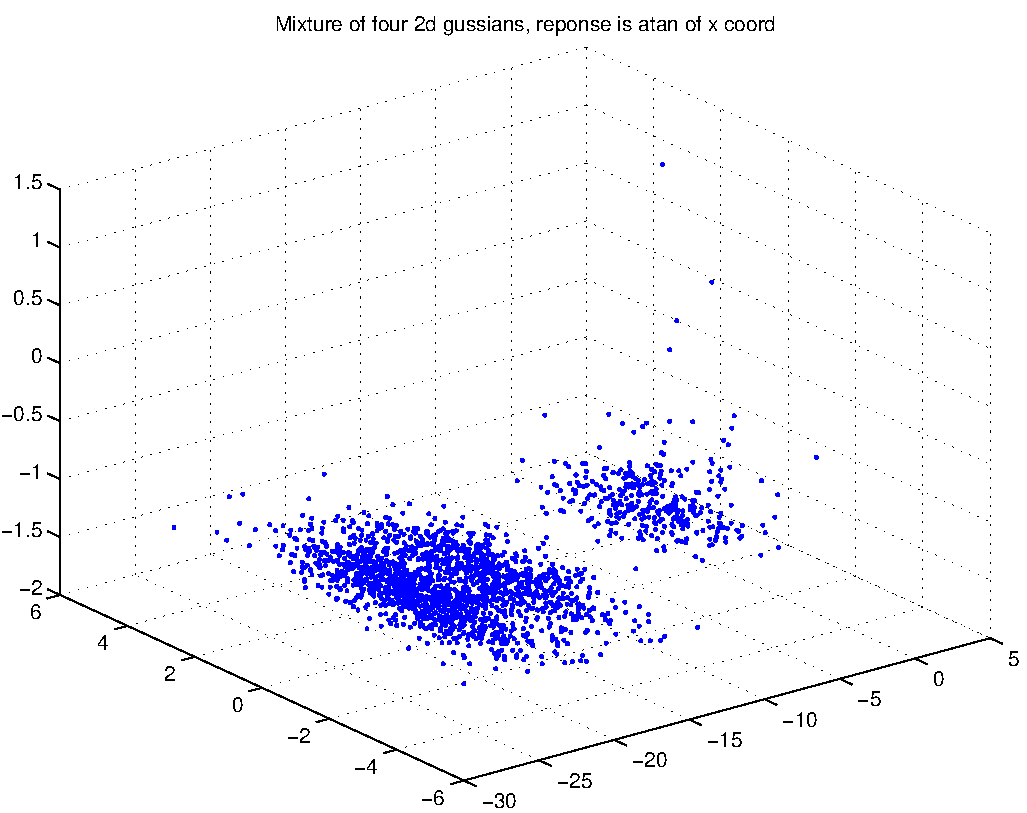
\includegraphics[width=10.0cm,height=10.0cm]{AtanDataSet.pdf}

\subsubsection{3 x 1 Linear Regression}
Sample size = 64

Number of features = 3

$\sigma = \left(
\begin{array}{
ccc}
+3.952 & -0.499 & -0.010 \\
-0.499 & +1.895 & +0.465 \\
-0.010 & +0.465 & +4.477 \\
\end{array}
\right)$ \newline 

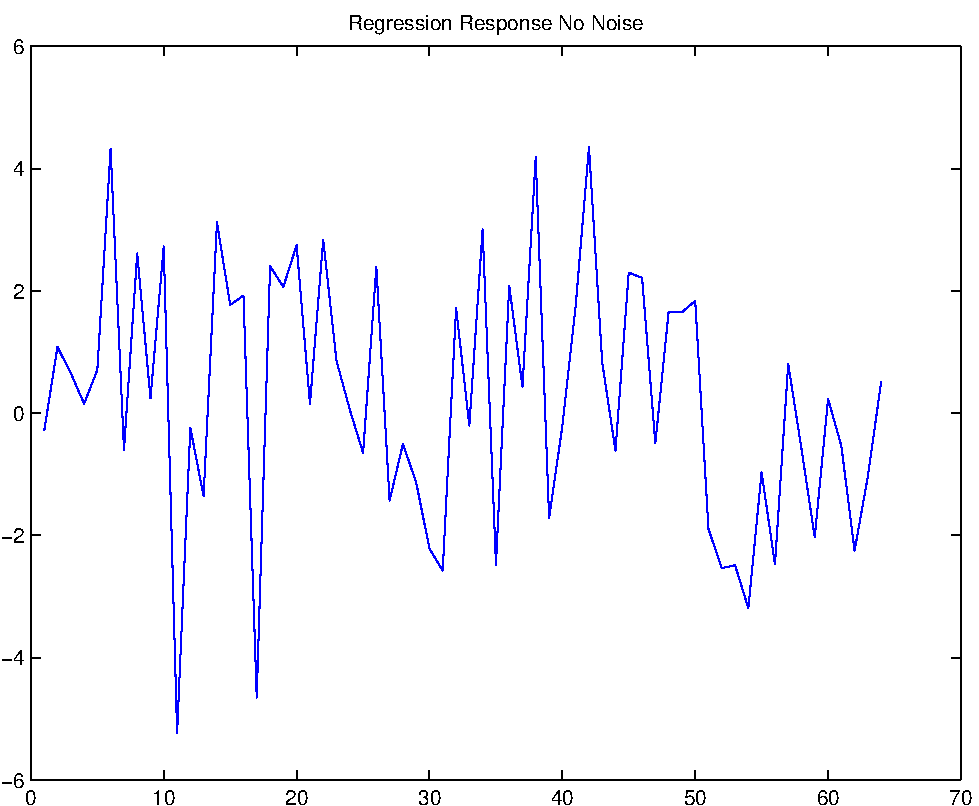
\includegraphics[width=10.0cm,height=10.0cm]{regression_response_no_noise.pdf}

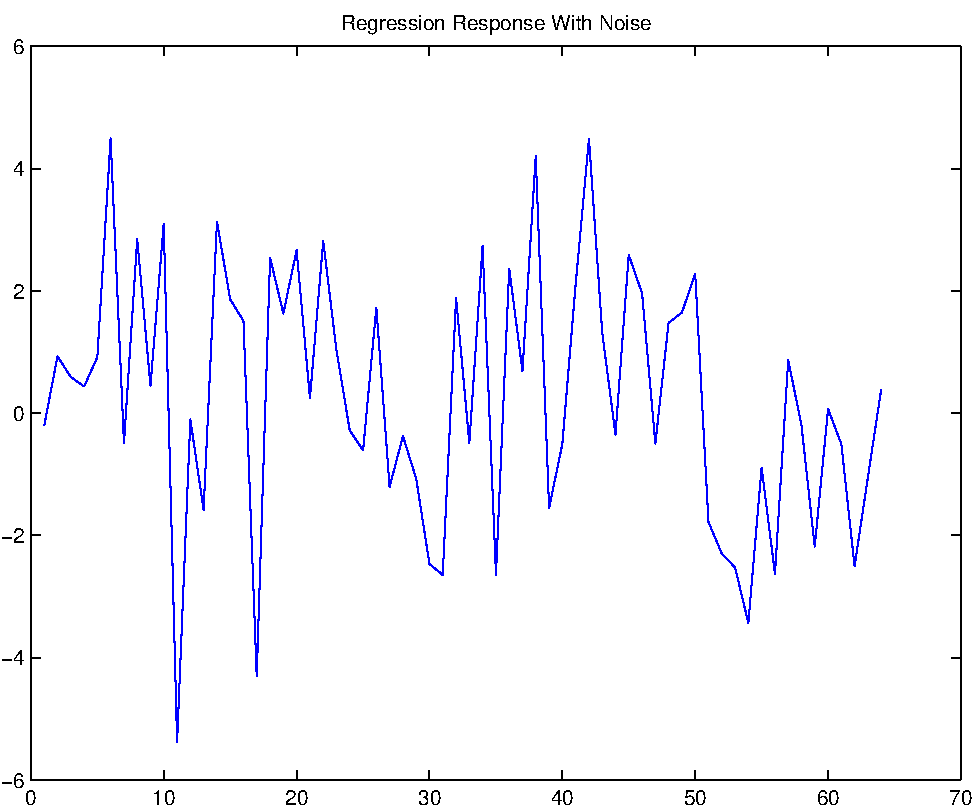
\includegraphics[width=10.0cm,height=10.0cm]{regression_response_with_noise.pdf}

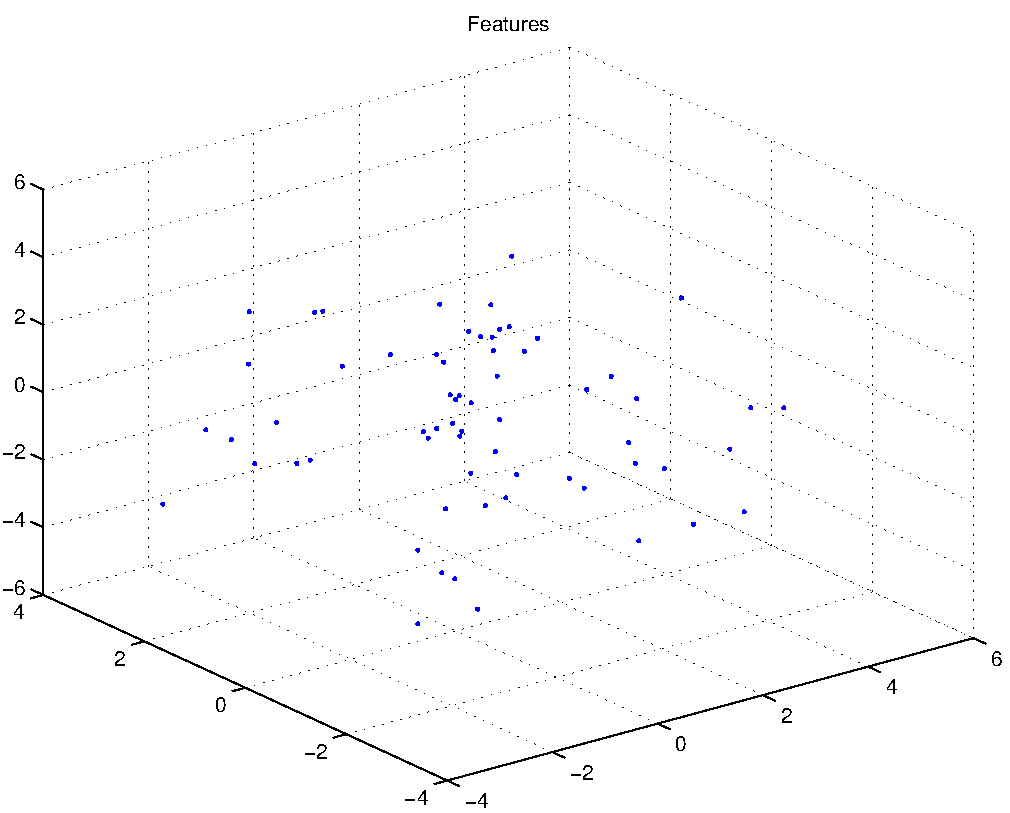
\includegraphics[width=10.0cm,height=10.0cm]{regression_features.pdf}

Beta
+0.817, +0.999, +0.510

Response
-1.267
+1.782
+1.082
+2.309
+1.107
+2.773
-0.979
+2.769
-2.248
+1.448
+2.213
+2.642
-4.235
+1.430
+2.485
+3.870
-1.652
+4.646
+1.139
+0.557
-1.426
+1.914
-0.581
-1.438
+0.134
+1.716
+1.994
+1.099
+3.113
+0.416
-1.680
-0.558
-1.345
+4.313
-2.862
+0.853
+6.741
-1.304
-1.125
+0.530
+0.442
+1.794
+2.476
+3.543
-5.174
+2.167
+0.423
-1.267
+0.327
+0.543
-1.660
-3.110
-1.500
+0.367
+2.692
-0.142
-2.000
+5.808
+1.208
+0.099
+3.734
-0.400
-0.644
-1.425
Estimate for Beta
+0.822
+1.006
+0.507
Error:
+0.004, +0.007, -0.004


QueryPerformanceCounter  =  +4.608
\subsubsection{Fast Gauss Transform}
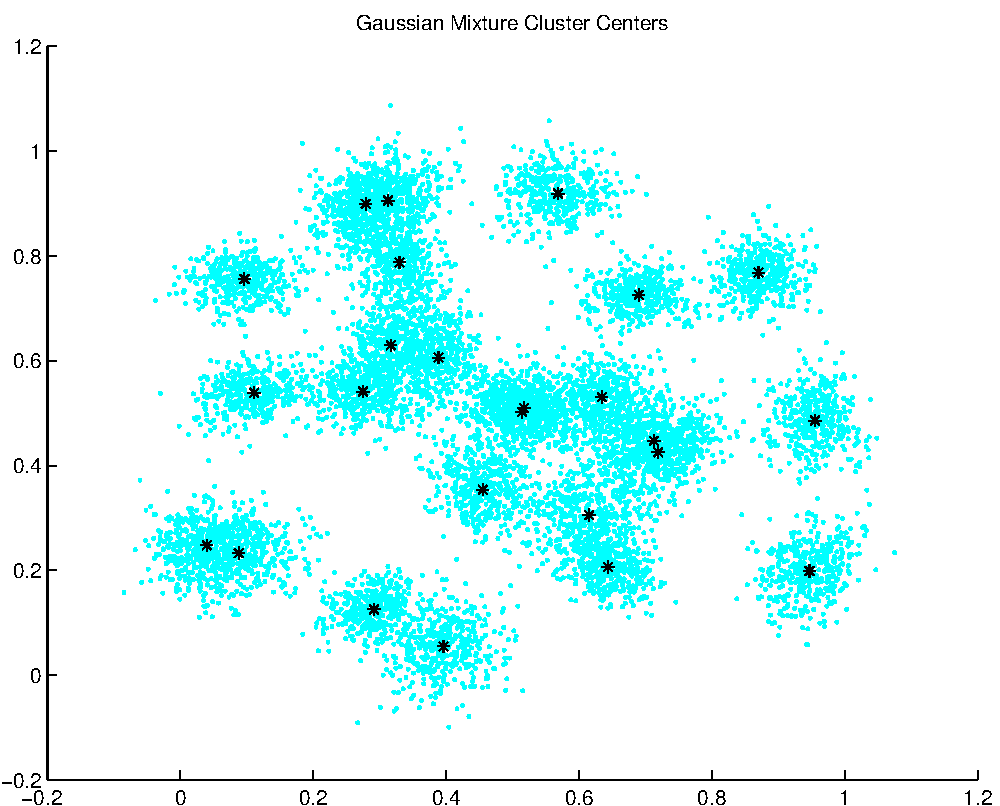
\includegraphics[width=10.0cm,height=10.0cm]{GaussianMixture_ClusterCenters25_Centers.pdf}

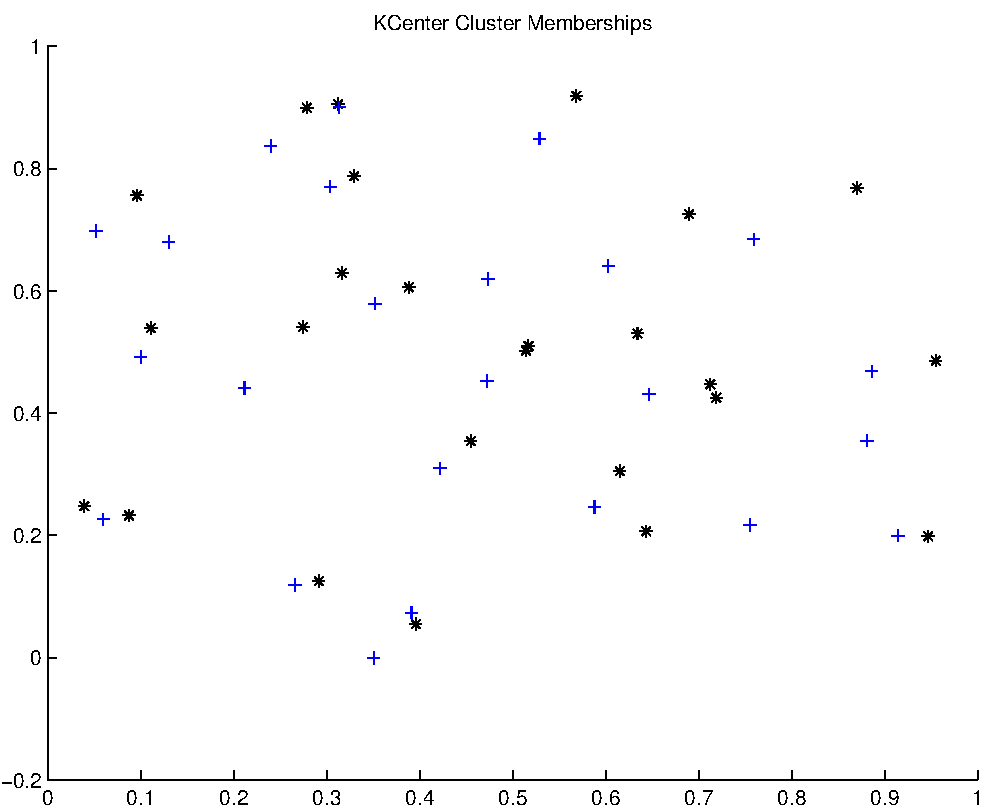
\includegraphics[width=10.0cm,height=10.0cm]{KCenterClusterMemberships_25_Centers.pdf}

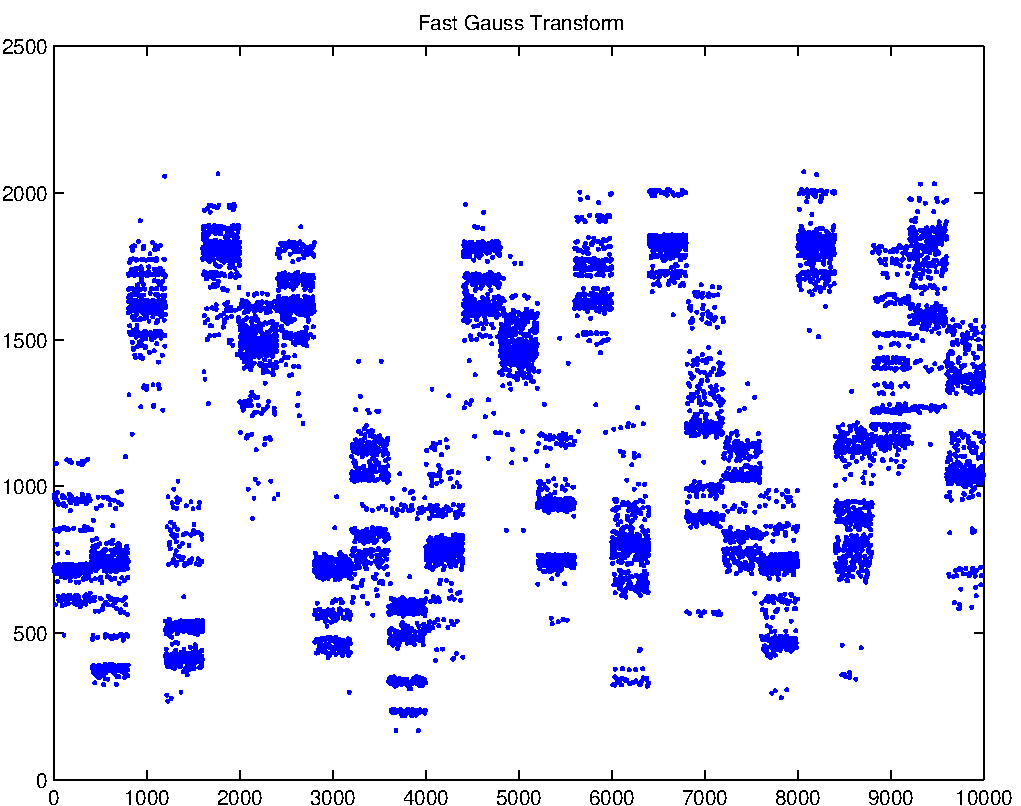
\includegraphics[width=10.0cm,height=10.0cm]{FGT25_Centers.pdf}

QueryPerformanceCounter  =  +7.350
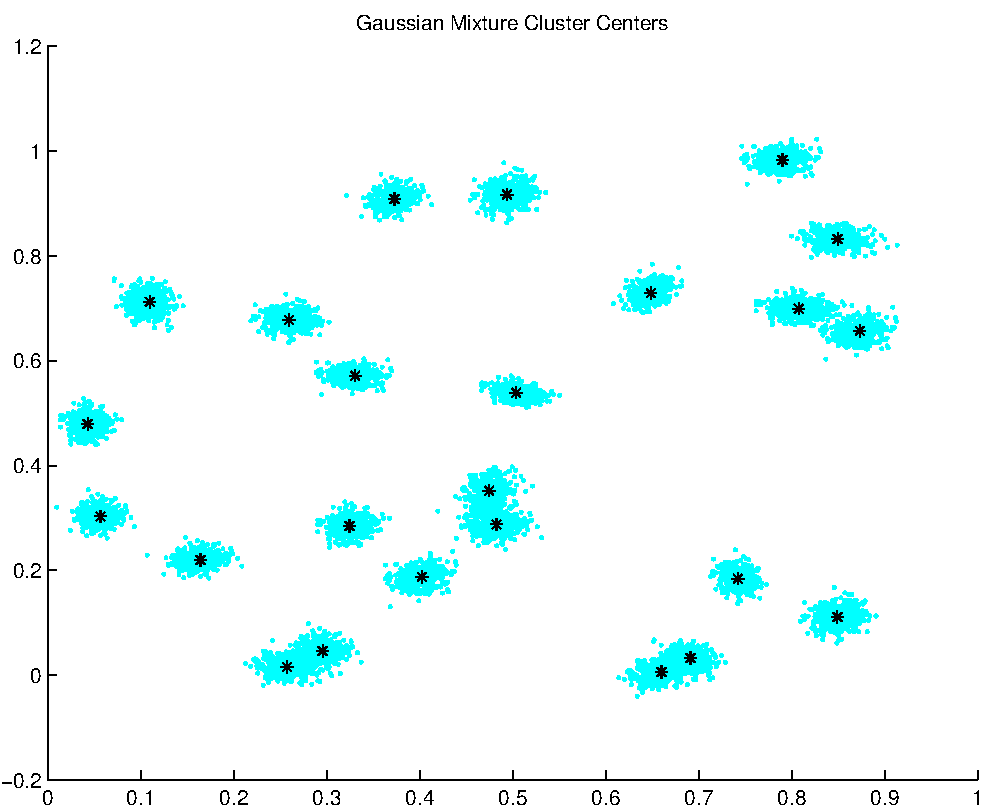
\includegraphics[width=10.0cm,height=10.0cm]{GaussianMixture_ClusterCenters24_Centers.pdf}

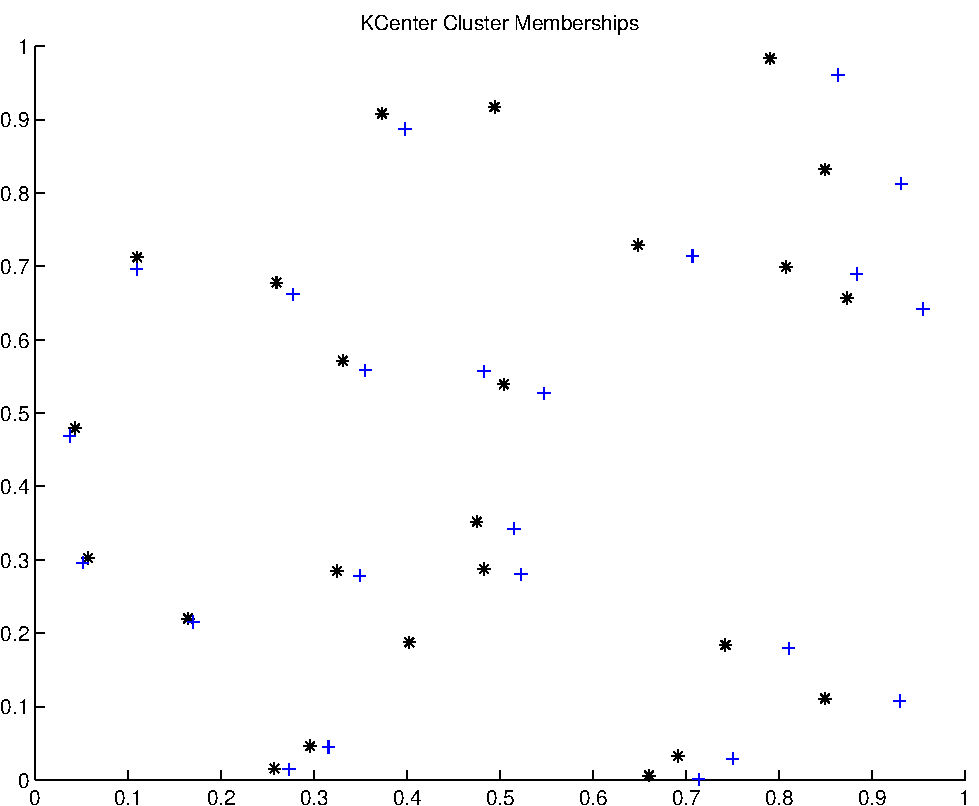
\includegraphics[width=10.0cm,height=10.0cm]{KCenterClusterMemberships_24_Centers.pdf}

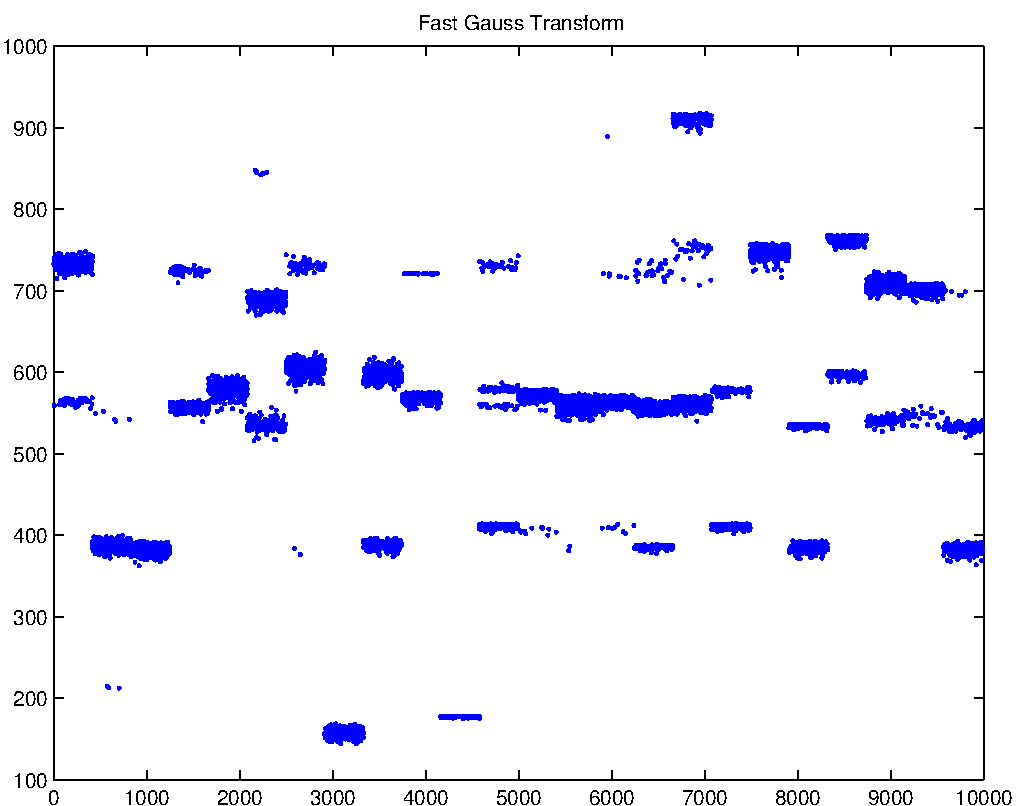
\includegraphics[width=10.0cm,height=10.0cm]{FGT24_Centers.pdf}

QueryPerformanceCounter  =  +7.498
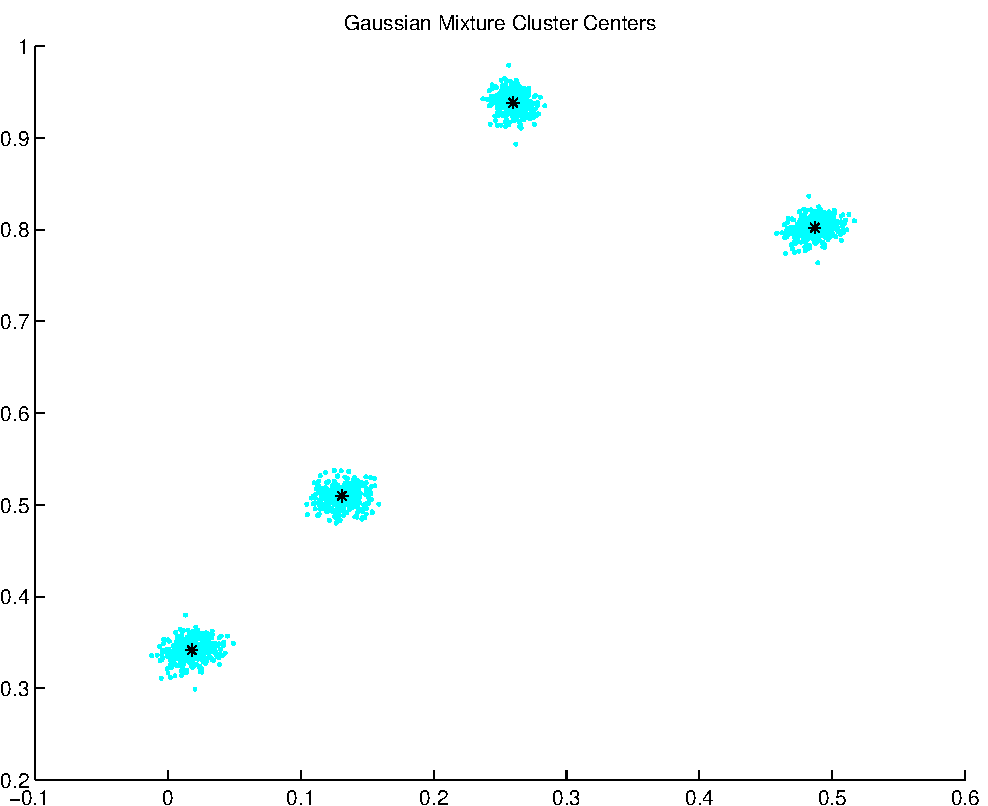
\includegraphics[width=10.0cm,height=10.0cm]{GaussianMixture_ClusterCenters4_Centers.pdf}

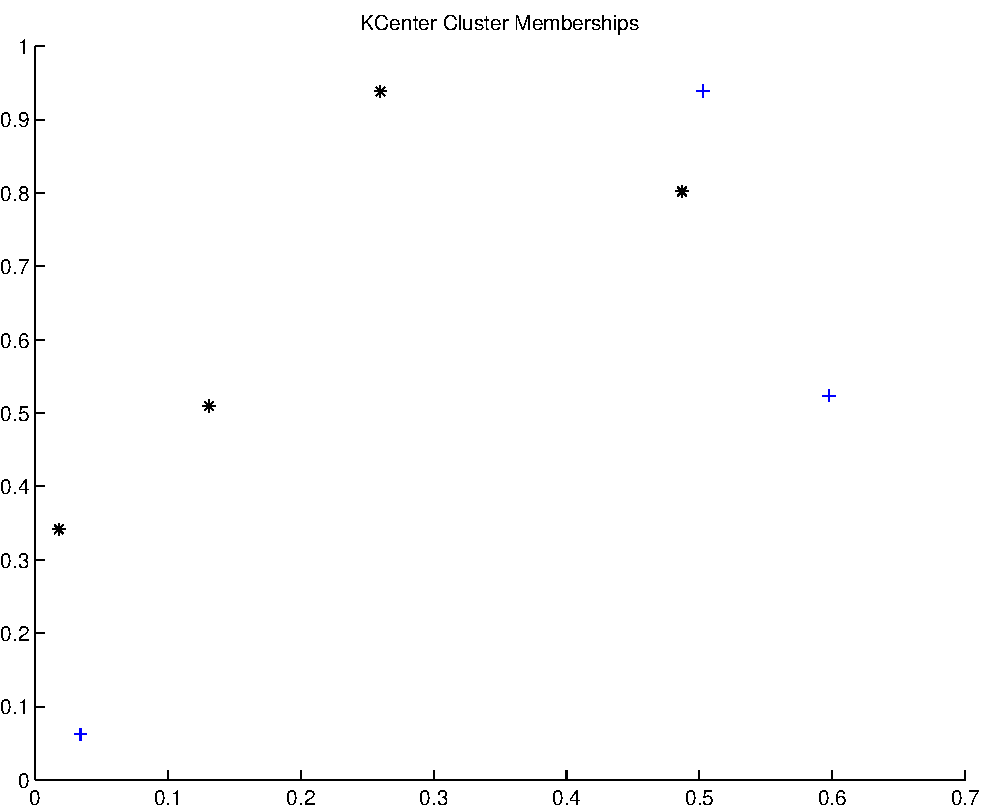
\includegraphics[width=10.0cm,height=10.0cm]{KCenterClusterMemberships_4_Centers.pdf}

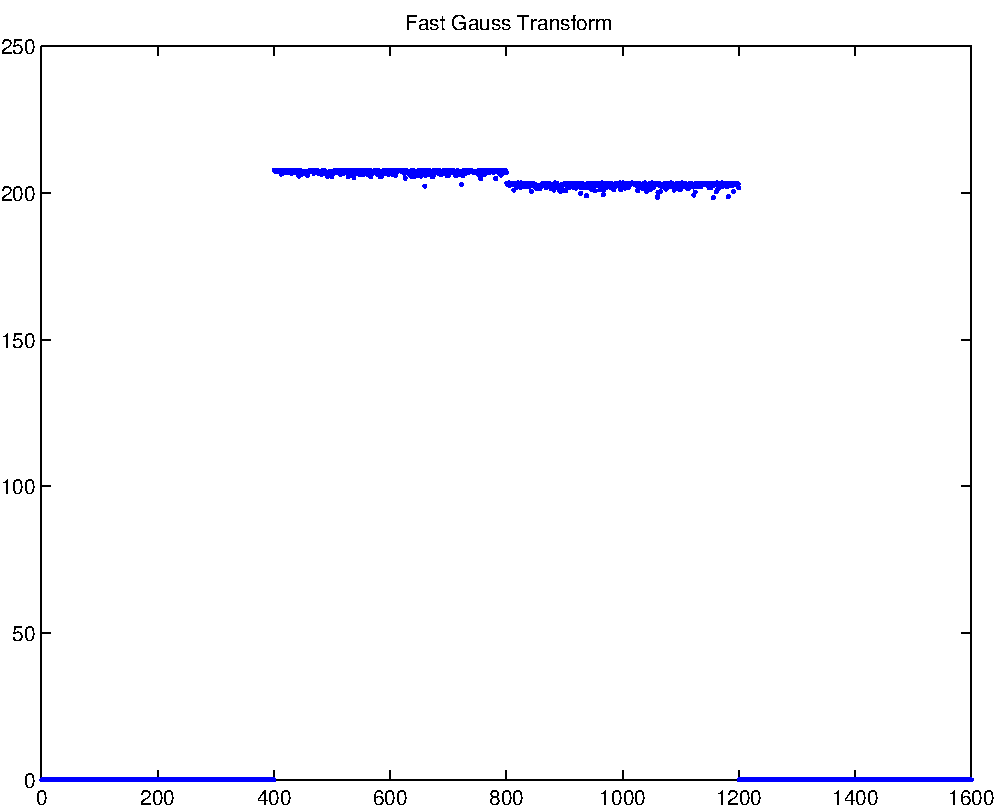
\includegraphics[width=10.0cm,height=10.0cm]{FGT4_Centers.pdf}

QueryPerformanceCounter  =  +3.724
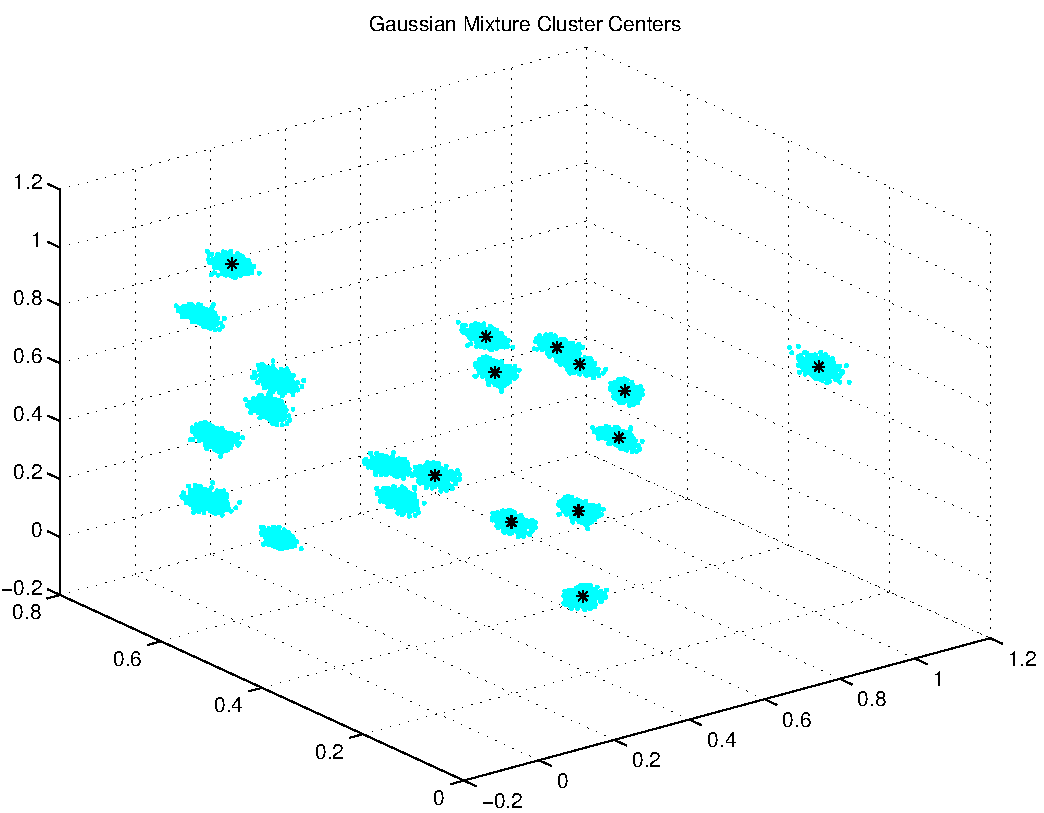
\includegraphics[width=10.0cm,height=10.0cm]{GaussianMixture_ClusterCenters20_Centers.pdf}

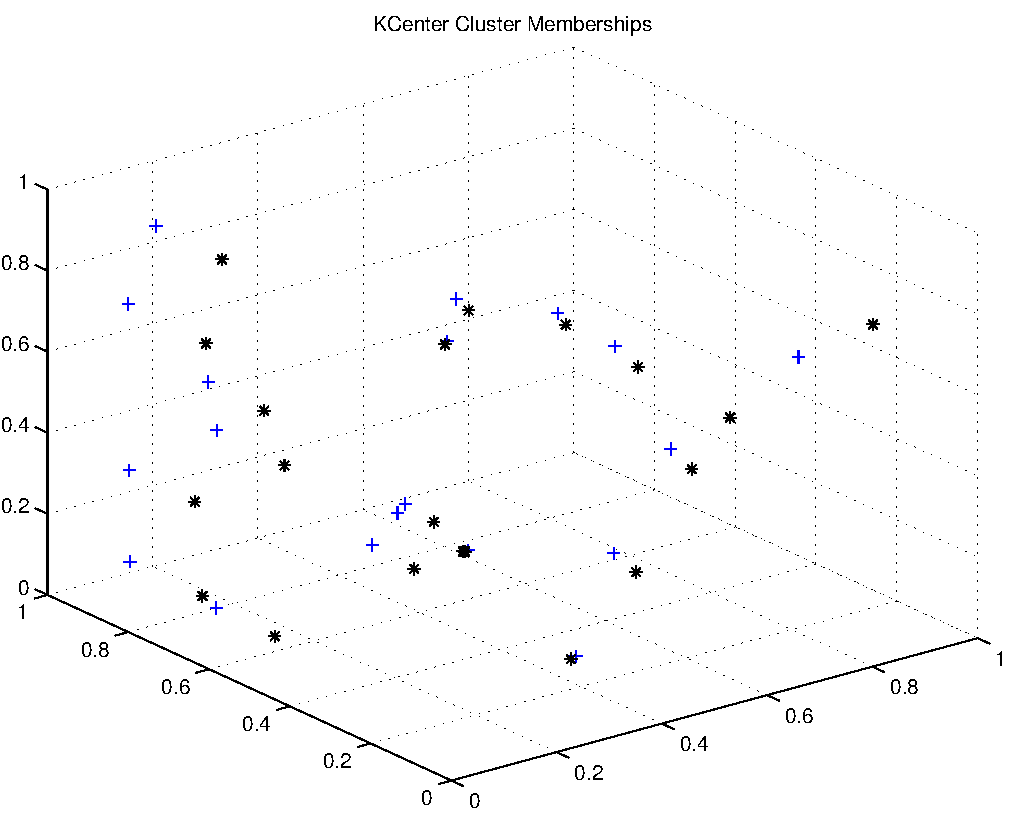
\includegraphics[width=10.0cm,height=10.0cm]{KCenterClusterMemberships_20_Centers.pdf}

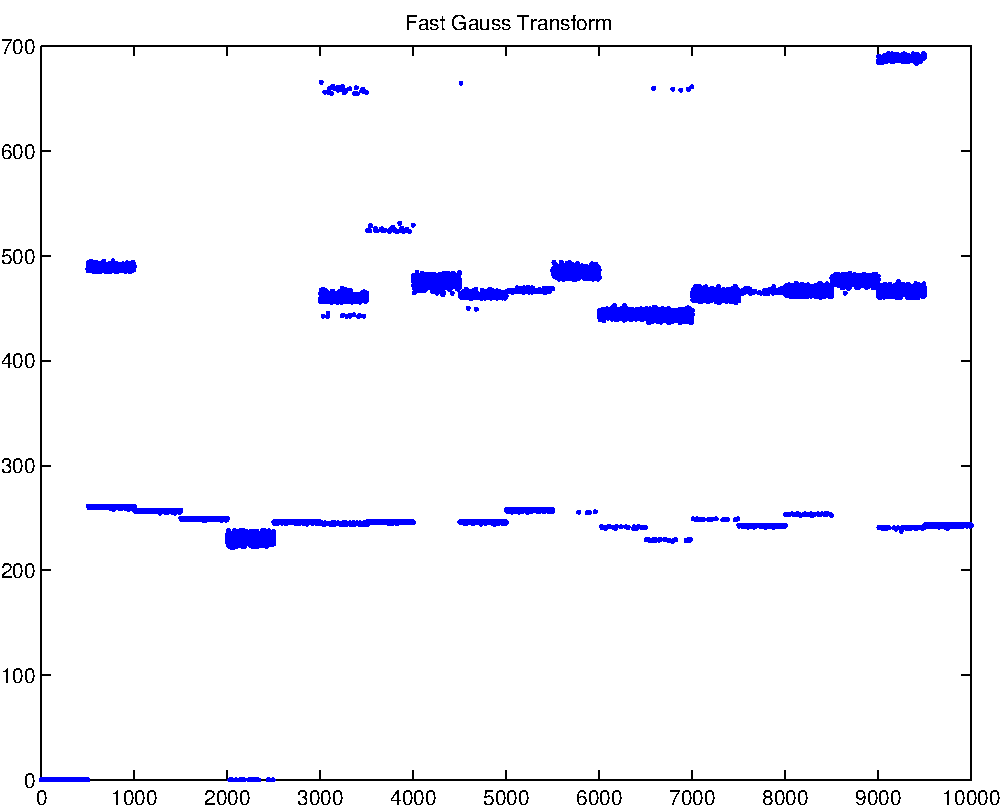
\includegraphics[width=10.0cm,height=10.0cm]{FGT20_Centers.pdf}

QueryPerformanceCounter  =  +6.190
\subsubsection{Matrix Norms}
\subsubsection{Haar Distributed Random Orthogonal Matrix $A \in O(n)$}
 Testing Operator Norm
Number of Dimensions: +12

$A = \left(
\begin{array}{
cccccccccccc}
+0.367 & +0.129 & +0.449 & +0.081 & -0.087 & -0.257 & +0.241 & -0.035 & +0.512 & +0.323 & -0.073 & -0.368 \\
-0.084 & +0.237 & -0.160 & +0.050 & +0.148 & +0.355 & -0.164 & -0.387 & -0.210 & +0.676 & +0.121 & -0.262 \\
-0.497 & -0.281 & +0.225 & +0.372 & +0.139 & +0.462 & +0.336 & +0.258 & +0.183 & +0.097 & -0.170 & -0.026 \\
+0.281 & -0.370 & +0.423 & -0.193 & -0.057 & +0.213 & +0.364 & -0.354 & -0.317 & +0.030 & +0.275 & +0.291 \\
-0.205 & +0.255 & +0.142 & -0.112 & -0.504 & -0.028 & +0.251 & -0.082 & -0.455 & -0.090 & -0.497 & -0.269 \\
+0.210 & +0.024 & +0.137 & +0.844 & -0.247 & -0.028 & -0.257 & -0.083 & -0.228 & -0.139 & +0.131 & +0.024 \\
-0.189 & +0.529 & +0.286 & -0.039 & -0.126 & -0.094 & +0.041 & +0.402 & -0.091 & +0.286 & +0.294 & +0.487 \\
-0.106 & +0.163 & +0.438 & +0.039 & +0.720 & -0.254 & -0.134 & -0.139 & -0.261 & -0.154 & -0.236 & -0.025 \\
-0.049 & -0.508 & +0.131 & -0.105 & -0.057 & -0.295 & -0.256 & +0.459 & -0.354 & +0.325 & +0.124 & -0.313 \\
-0.172 & -0.215 & +0.267 & -0.115 & -0.261 & +0.011 & -0.555 & -0.264 & +0.262 & +0.187 & -0.387 & +0.374 \\
+0.601 & +0.085 & -0.005 & -0.057 & +0.124 & +0.451 & -0.124 & +0.420 & -0.132 & +0.073 & -0.427 & +0.111 \\
+0.078 & -0.164 & -0.377 & +0.244 & +0.109 & -0.429 & +0.364 & -0.072 & -0.110 & +0.386 & -0.348 & +0.387 \\
\end{array}
\right)$ \newline 

$Det(A) :   A \in O(n)$ = (+1.000,-0.000)

$L = \left(
\begin{array}{
cccccccccccc}
+1.000 & +0.000 & +0.000 & +0.000 & +0.000 & +0.000 & +0.000 & +0.000 & +0.000 & +0.000 & +0.000 & +0.000 \\
-0.314 & +1.000 & +0.000 & +0.000 & +0.000 & +0.000 & +0.000 & +0.000 & +0.000 & +0.000 & +0.000 & +0.000 \\
+0.467 & -0.737 & +1.000 & +0.000 & +0.000 & +0.000 & +0.000 & +0.000 & +0.000 & +0.000 & +0.000 & +0.000 \\
+0.350 & -0.010 & +0.223 & +1.000 & +0.000 & +0.000 & +0.000 & +0.000 & +0.000 & +0.000 & +0.000 & +0.000 \\
-0.176 & +0.321 & +0.545 & +0.177 & +1.000 & +0.000 & +0.000 & +0.000 & +0.000 & +0.000 & +0.000 & +0.000 \\
-0.828 & -0.379 & +0.518 & +0.451 & +0.455 & +1.000 & +0.000 & +0.000 & +0.000 & +0.000 & +0.000 & +0.000 \\
-0.286 & -0.344 & +0.572 & -0.035 & -0.178 & +0.097 & +1.000 & +0.000 & +0.000 & +0.000 & +0.000 & +0.000 \\
-0.082 & -0.903 & +0.609 & -0.038 & -0.029 & -0.250 & +0.501 & +1.000 & +0.000 & +0.000 & +0.000 & +0.000 \\
+0.611 & +0.139 & +0.650 & +0.284 & +0.040 & -0.501 & -0.317 & +0.236 & +1.000 & +0.000 & +0.000 & +0.000 \\
-0.139 & +0.447 & -0.453 & -0.029 & +0.127 & +0.429 & +0.095 & -0.813 & -0.652 & +1.000 & +0.000 & +0.000 \\
-0.341 & +0.512 & -0.008 & -0.114 & -0.491 & -0.007 & -0.017 & -0.217 & -0.446 & -0.154 & +1.000 & +0.000 \\
+0.130 & -0.316 & -0.451 & +0.153 & +0.026 & -0.421 & -0.812 & +0.333 & +0.201 & +0.570 & +0.696 & +1.000 \\
\end{array}
\right)$ \newline 

$U = \left(
\begin{array}{
cccccccccccc}
+0.601 & +0.085 & -0.005 & -0.057 & +0.124 & +0.451 & -0.124 & +0.420 & -0.132 & +0.073 & -0.427 & +0.111 \\
+0.000 & +0.556 & +0.284 & -0.057 & -0.087 & +0.048 & +0.002 & +0.534 & -0.132 & +0.309 & +0.160 & +0.522 \\
+0.000 & +0.000 & +0.635 & -0.208 & -0.179 & +0.037 & +0.423 & -0.157 & -0.353 & +0.224 & +0.593 & +0.624 \\
+0.000 & +0.000 & +0.000 & +0.910 & -0.251 & -0.194 & -0.308 & -0.190 & -0.104 & -0.211 & +0.149 & -0.149 \\
+0.000 & +0.000 & +0.000 & +0.000 & +0.912 & -0.176 & -0.332 & -0.118 & -0.031 & -0.325 & -0.712 & -0.486 \\
+0.000 & +0.000 & +0.000 & +0.000 & +0.000 & +1.002 & +0.305 & +1.029 & +0.267 & +0.402 & -0.514 & +0.229 \\
+0.000 & +0.000 & +0.000 & +0.000 & +0.000 & +0.000 & -0.931 & +0.001 & +0.346 & +0.082 & -0.864 & +0.115 \\
+0.000 & +0.000 & +0.000 & +0.000 & +0.000 & +0.000 & +0.000 & +1.316 & -0.381 & +0.516 & +0.163 & -0.233 \\
+0.000 & +0.000 & +0.000 & +0.000 & +0.000 & +0.000 & +0.000 & +0.000 & +1.205 & +0.268 & -0.802 & -0.646 \\
+0.000 & +0.000 & +0.000 & +0.000 & +0.000 & +0.000 & +0.000 & +0.000 & +0.000 & +1.099 & +0.265 & -0.859 \\
+0.000 & +0.000 & +0.000 & +0.000 & +0.000 & +0.000 & +0.000 & +0.000 & +0.000 & +0.000 & -1.352 & -1.217 \\
+0.000 & +0.000 & +0.000 & +0.000 & +0.000 & +0.000 & +0.000 & +0.000 & +0.000 & +0.000 & +0.000 & +2.587 \\
\end{array}
\right)$ \newline 

$L * U  = \left(
\begin{array}{
cccccccccccc}
+0.601 & +0.085 & -0.005 & -0.057 & +0.124 & +0.451 & -0.124 & +0.420 & -0.132 & +0.073 & -0.427 & +0.111 \\
-0.189 & +0.529 & +0.286 & -0.039 & -0.126 & -0.094 & +0.041 & +0.402 & -0.091 & +0.286 & +0.294 & +0.487 \\
+0.281 & -0.370 & +0.423 & -0.193 & -0.057 & +0.213 & +0.364 & -0.354 & -0.317 & +0.030 & +0.275 & +0.291 \\
+0.210 & +0.024 & +0.137 & +0.844 & -0.247 & -0.028 & -0.257 & -0.083 & -0.228 & -0.139 & +0.131 & +0.024 \\
-0.106 & +0.163 & +0.438 & +0.039 & +0.720 & -0.254 & -0.134 & -0.139 & -0.261 & -0.154 & -0.236 & -0.025 \\
-0.497 & -0.281 & +0.225 & +0.372 & +0.139 & +0.462 & +0.336 & +0.258 & +0.183 & +0.097 & -0.170 & -0.026 \\
-0.172 & -0.215 & +0.267 & -0.115 & -0.261 & +0.011 & -0.555 & -0.264 & +0.262 & +0.187 & -0.387 & +0.374 \\
-0.049 & -0.508 & +0.131 & -0.105 & -0.057 & -0.295 & -0.256 & +0.459 & -0.354 & +0.325 & +0.124 & -0.313 \\
+0.367 & +0.129 & +0.449 & +0.081 & -0.087 & -0.257 & +0.241 & -0.035 & +0.512 & +0.323 & -0.073 & -0.368 \\
-0.084 & +0.237 & -0.160 & +0.050 & +0.148 & +0.355 & -0.164 & -0.387 & -0.210 & +0.676 & +0.121 & -0.262 \\
-0.205 & +0.255 & +0.142 & -0.112 & -0.504 & -0.028 & +0.251 & -0.082 & -0.455 & -0.090 & -0.497 & -0.269 \\
+0.078 & -0.164 & -0.377 & +0.244 & +0.109 & -0.429 & +0.364 & -0.072 & -0.110 & +0.386 & -0.348 & +0.387 \\
\end{array}
\right)$ \newline 

$Det(L) :    = (+1.000,+0.000)     Det(U) :    = (+1.000,+0.000)     Det(LU) :    = (+1.000,-0.000)$

$||A||_{L_1}$  = +3.116

$||A||_{L_{\infty}}$ = +3.167

$||A^{-1}||_{L_1}$  = +3.167

$||A^{-1}||_{L_{\infty}}$ = +3.116

$||A||_{L_{\infty}} * ||A^{-1}||_{L_{\infty}} = +9.871$

$||A||_{L_1} * ||A^{-1}||_{L_1} = +9.871$

Frobenious Norm  $||A||_{\textit{F}}$ via $\sum\limits_{i,j =0}^{n} \|A_{i,j}|$   of  $A \in O(n)$  +3.464

$L_1$ condition number of Haar Distributed Random Orthogonal Matrix $A \in O(n)$ +8.135

$A = \left(
\begin{array}{
cccccccccccc}
+0.367 & +0.129 & +0.449 & +0.081 & -0.087 & -0.257 & +0.241 & -0.035 & +0.512 & +0.323 & -0.073 & -0.368 \\
-0.084 & +0.237 & -0.160 & +0.050 & +0.148 & +0.355 & -0.164 & -0.387 & -0.210 & +0.676 & +0.121 & -0.262 \\
-0.497 & -0.281 & +0.225 & +0.372 & +0.139 & +0.462 & +0.336 & +0.258 & +0.183 & +0.097 & -0.170 & -0.026 \\
+0.281 & -0.370 & +0.423 & -0.193 & -0.057 & +0.213 & +0.364 & -0.354 & -0.317 & +0.030 & +0.275 & +0.291 \\
-0.205 & +0.255 & +0.142 & -0.112 & -0.504 & -0.028 & +0.251 & -0.082 & -0.455 & -0.090 & -0.497 & -0.269 \\
+0.210 & +0.024 & +0.137 & +0.844 & -0.247 & -0.028 & -0.257 & -0.083 & -0.228 & -0.139 & +0.131 & +0.024 \\
-0.189 & +0.529 & +0.286 & -0.039 & -0.126 & -0.094 & +0.041 & +0.402 & -0.091 & +0.286 & +0.294 & +0.487 \\
-0.106 & +0.163 & +0.438 & +0.039 & +0.720 & -0.254 & -0.134 & -0.139 & -0.261 & -0.154 & -0.236 & -0.025 \\
-0.049 & -0.508 & +0.131 & -0.105 & -0.057 & -0.295 & -0.256 & +0.459 & -0.354 & +0.325 & +0.124 & -0.313 \\
-0.172 & -0.215 & +0.267 & -0.115 & -0.261 & +0.011 & -0.555 & -0.264 & +0.262 & +0.187 & -0.387 & +0.374 \\
+0.601 & +0.085 & -0.005 & -0.057 & +0.124 & +0.451 & -0.124 & +0.420 & -0.132 & +0.073 & -0.427 & +0.111 \\
+0.078 & -0.164 & -0.377 & +0.244 & +0.109 & -0.429 & +0.364 & -0.072 & -0.110 & +0.386 & -0.348 & +0.387 \\
\end{array}
\right)$ \newline 

$L_{\infty}$ condition number of Haar Distributed Random Orthogonal Matrix $A \in O(n)$ +7.130

Eigenvalues of $A \in O(n)$

(+0.385,+0.923), (+0.385,-0.923), (-0.340,+0.941), (-0.340,-0.941), (-0.867,+0.498), (-0.867,-0.498), (-0.963,+0.269), (-0.963,-0.269), (+0.942,+0.335), (+0.942,-0.335), (+0.741,+0.671), (+0.741,-0.671)

 $|\lambda | : \lambda \in \sigma(A) , A \in O(n)$

+1.000, +1.000, +1.000, +1.000, +1.000, +1.000, +1.000, +1.000, +1.000, +1.000, +1.000, +1.000


Calculating $A^{\dag} A,$  we expect $A^{\dag} A \approx I$

$A^{\dag} A = \left(
\begin{array}{
cccccccccccc}
+1.000 & -0.000 & +0.000 & -0.000 & +0.000 & +0.000 & +0.000 & +0.000 & -0.000 & +0.000 & +0.000 & +0.000 \\
-0.000 & +1.000 & -0.000 & +0.000 & -0.000 & +0.000 & +0.000 & +0.000 & -0.000 & -0.000 & +0.000 & +0.000 \\
+0.000 & -0.000 & +1.000 & -0.000 & +0.000 & -0.000 & +0.000 & -0.000 & -0.000 & -0.000 & +0.000 & -0.000 \\
-0.000 & +0.000 & -0.000 & +1.000 & +0.000 & -0.000 & -0.000 & +0.000 & +0.000 & +0.000 & +0.000 & -0.000 \\
+0.000 & -0.000 & +0.000 & +0.000 & +1.000 & +0.000 & -0.000 & +0.000 & +0.000 & -0.000 & +0.000 & +0.000 \\
+0.000 & +0.000 & -0.000 & -0.000 & +0.000 & +1.000 & +0.000 & +0.000 & -0.000 & +0.000 & -0.000 & +0.000 \\
+0.000 & +0.000 & +0.000 & -0.000 & -0.000 & +0.000 & +1.000 & +0.000 & -0.000 & -0.000 & +0.000 & -0.000 \\
+0.000 & +0.000 & -0.000 & +0.000 & +0.000 & +0.000 & +0.000 & +1.000 & -0.000 & -0.000 & -0.000 & -0.000 \\
-0.000 & -0.000 & -0.000 & +0.000 & +0.000 & -0.000 & -0.000 & -0.000 & +1.000 & -0.000 & -0.000 & +0.000 \\
+0.000 & -0.000 & -0.000 & +0.000 & -0.000 & +0.000 & -0.000 & -0.000 & -0.000 & +1.000 & +0.000 & -0.000 \\
+0.000 & +0.000 & +0.000 & +0.000 & +0.000 & -0.000 & +0.000 & -0.000 & -0.000 & +0.000 & +1.000 & -0.000 \\
+0.000 & +0.000 & -0.000 & -0.000 & +0.000 & +0.000 & -0.000 & -0.000 & +0.000 & -0.000 & -0.000 & +1.000 \\
\end{array}
\right)$ \newline 

Calculating $A^{-1} ,  A \in O(n)$.

$A^{-1} = \left(
\begin{array}{
cccccccccccc}
+0.367 & -0.084 & -0.497 & +0.281 & -0.205 & +0.210 & -0.189 & -0.106 & -0.049 & -0.172 & +0.601 & +0.078 \\
+0.129 & +0.237 & -0.281 & -0.370 & +0.255 & +0.024 & +0.529 & +0.163 & -0.508 & -0.215 & +0.085 & -0.164 \\
+0.449 & -0.160 & +0.225 & +0.423 & +0.142 & +0.137 & +0.286 & +0.438 & +0.131 & +0.267 & -0.005 & -0.377 \\
+0.081 & +0.050 & +0.372 & -0.193 & -0.112 & +0.844 & -0.039 & +0.039 & -0.105 & -0.115 & -0.057 & +0.244 \\
-0.087 & +0.148 & +0.139 & -0.057 & -0.504 & -0.247 & -0.126 & +0.720 & -0.057 & -0.261 & +0.124 & +0.109 \\
-0.257 & +0.355 & +0.462 & +0.213 & -0.028 & -0.028 & -0.094 & -0.254 & -0.295 & +0.011 & +0.451 & -0.429 \\
+0.241 & -0.164 & +0.336 & +0.364 & +0.251 & -0.257 & +0.041 & -0.134 & -0.256 & -0.555 & -0.124 & +0.364 \\
-0.035 & -0.387 & +0.258 & -0.354 & -0.082 & -0.083 & +0.402 & -0.139 & +0.459 & -0.264 & +0.420 & -0.072 \\
+0.512 & -0.210 & +0.183 & -0.317 & -0.455 & -0.228 & -0.091 & -0.261 & -0.354 & +0.262 & -0.132 & -0.110 \\
+0.323 & +0.676 & +0.097 & +0.030 & -0.090 & -0.139 & +0.286 & -0.154 & +0.325 & +0.187 & +0.073 & +0.386 \\
-0.073 & +0.121 & -0.170 & +0.275 & -0.497 & +0.131 & +0.294 & -0.236 & +0.124 & -0.387 & -0.427 & -0.348 \\
-0.368 & -0.262 & -0.026 & +0.291 & -0.269 & +0.024 & +0.487 & -0.025 & -0.313 & +0.374 & +0.111 & +0.387 \\
\end{array}
\right)$ \newline 

Calculating $A^{-1} *A  ,  A \in O(n)$.   We expect $A^{-1} *A  \approx I$. 

$A^{-1} *A = \left(
\begin{array}{
cccccccccccc}
+1.000 & +0.000 & +0.000 & +0.000 & -0.000 & -0.000 & +0.000 & +0.000 & -0.000 & +0.000 & +0.000 & +0.000 \\
-0.000 & +1.000 & +0.000 & -0.000 & -0.000 & +0.000 & +0.000 & -0.000 & +0.000 & -0.000 & -0.000 & +0.000 \\
+0.000 & -0.000 & +1.000 & -0.000 & +0.000 & +0.000 & +0.000 & +0.000 & +0.000 & +0.000 & -0.000 & +0.000 \\
-0.000 & +0.000 & +0.000 & +1.000 & +0.000 & +0.000 & -0.000 & +0.000 & +0.000 & -0.000 & +0.000 & -0.000 \\
-0.000 & +0.000 & +0.000 & +0.000 & +1.000 & +0.000 & +0.000 & +0.000 & +0.000 & +0.000 & +0.000 & +0.000 \\
-0.000 & -0.000 & -0.000 & -0.000 & +0.000 & +1.000 & +0.000 & +0.000 & +0.000 & -0.000 & -0.000 & +0.000 \\
-0.000 & -0.000 & -0.000 & +0.000 & +0.000 & +0.000 & +1.000 & +0.000 & +0.000 & +0.000 & -0.000 & +0.000 \\
-0.000 & -0.000 & -0.000 & +0.000 & +0.000 & +0.000 & -0.000 & +1.000 & +0.000 & +0.000 & -0.000 & +0.000 \\
+0.000 & +0.000 & -0.000 & +0.000 & +0.000 & +0.000 & -0.000 & +0.000 & +1.000 & +0.000 & +0.000 & -0.000 \\
+0.000 & +0.000 & -0.000 & -0.000 & -0.000 & +0.000 & +0.000 & -0.000 & -0.000 & +1.000 & +0.000 & -0.000 \\
-0.000 & -0.000 & -0.000 & -0.000 & -0.000 & +0.000 & -0.000 & -0.000 & -0.000 & -0.000 & +1.000 & +0.000 \\
-0.000 & +0.000 & +0.000 & -0.000 & +0.000 & -0.000 & +0.000 & +0.000 & -0.000 & -0.000 & +0.000 & +1.000 \\
\end{array}
\right)$ \newline 

Calculating SVD of  $A \in O(n)$

$U = \left(
\begin{array}{
cccccccccccc}
+0.163 & +0.255 & +0.296 & +0.405 & -0.378 & +0.424 & -0.275 & -0.143 & -0.329 & -0.005 & +0.303 & -0.193 \\
-0.095 & -0.132 & -0.292 & +0.082 & -0.150 & +0.052 & -0.151 & +0.567 & +0.305 & +0.353 & +0.542 & -0.006 \\
-0.033 & -0.162 & -0.443 & +0.102 & -0.523 & -0.359 & -0.029 & -0.435 & +0.179 & -0.277 & +0.114 & -0.227 \\
+0.199 & -0.398 & -0.327 & +0.051 & +0.208 & +0.353 & +0.406 & -0.188 & -0.245 & +0.326 & +0.009 & -0.398 \\
+0.070 & -0.077 & +0.026 & -0.574 & -0.547 & +0.254 & -0.026 & +0.326 & -0.078 & -0.041 & -0.363 & -0.220 \\
+0.162 & +0.008 & -0.207 & +0.645 & -0.144 & -0.076 & +0.170 & +0.431 & -0.080 & -0.114 & -0.495 & +0.098 \\
-0.017 & -0.296 & +0.011 & +0.081 & -0.002 & -0.179 & -0.651 & -0.173 & -0.093 & +0.531 & -0.357 & +0.033 \\
-0.773 & -0.182 & +0.342 & +0.159 & -0.142 & -0.161 & +0.265 & +0.073 & -0.191 & +0.110 & -0.014 & -0.239 \\
+0.051 & -0.187 & +0.072 & +0.040 & +0.388 & -0.098 & -0.374 & +0.263 & +0.005 & -0.460 & +0.023 & -0.611 \\
-0.369 & +0.144 & -0.130 & +0.143 & +0.087 & +0.565 & -0.116 & -0.181 & +0.581 & -0.048 & -0.290 & -0.094 \\
-0.367 & -0.129 & -0.449 & -0.081 & +0.087 & +0.257 & -0.241 & +0.035 & -0.512 & -0.323 & +0.073 & +0.368 \\
+0.146 & -0.730 & +0.373 & +0.104 & -0.107 & +0.203 & +0.035 & -0.041 & +0.221 & -0.256 & +0.083 & +0.344 \\
\end{array}
\right)$ \newline 

$S = \left(
\begin{array}{
cccccccccccc}
+1.000 & +0.000 & +0.000 & +0.000 & +0.000 & +0.000 & +0.000 & +0.000 & +0.000 & +0.000 & +0.000 & +0.000 \\
+0.000 & +1.000 & +0.000 & +0.000 & +0.000 & +0.000 & +0.000 & +0.000 & +0.000 & +0.000 & +0.000 & +0.000 \\
+0.000 & +0.000 & +1.000 & +0.000 & +0.000 & +0.000 & +0.000 & +0.000 & +0.000 & +0.000 & +0.000 & +0.000 \\
+0.000 & +0.000 & +0.000 & +1.000 & +0.000 & +0.000 & +0.000 & +0.000 & +0.000 & +0.000 & +0.000 & +0.000 \\
+0.000 & +0.000 & +0.000 & +0.000 & +1.000 & +0.000 & +0.000 & +0.000 & +0.000 & +0.000 & +0.000 & +0.000 \\
+0.000 & +0.000 & +0.000 & +0.000 & +0.000 & +1.000 & +0.000 & +0.000 & +0.000 & +0.000 & +0.000 & +0.000 \\
+0.000 & +0.000 & +0.000 & +0.000 & +0.000 & +0.000 & +1.000 & +0.000 & +0.000 & +0.000 & +0.000 & +0.000 \\
+0.000 & +0.000 & +0.000 & +0.000 & +0.000 & +0.000 & +0.000 & +1.000 & +0.000 & +0.000 & +0.000 & +0.000 \\
+0.000 & +0.000 & +0.000 & +0.000 & +0.000 & +0.000 & +0.000 & +0.000 & +1.000 & +0.000 & +0.000 & +0.000 \\
+0.000 & +0.000 & +0.000 & +0.000 & +0.000 & +0.000 & +0.000 & +0.000 & +0.000 & +1.000 & +0.000 & +0.000 \\
+0.000 & +0.000 & +0.000 & +0.000 & +0.000 & +0.000 & +0.000 & +0.000 & +0.000 & +0.000 & +1.000 & +0.000 \\
+0.000 & +0.000 & +0.000 & +0.000 & +0.000 & +0.000 & +0.000 & +0.000 & +0.000 & +0.000 & +0.000 & +1.000 \\
\end{array}
\right)$ \newline 

$V = \left(
\begin{array}{
cccccccccccc}
+0.000 & +0.000 & +0.000 & -0.000 & +0.000 & -0.000 & -0.000 & +0.000 & +0.000 & +0.000 & -1.000 & -0.000 \\
+0.368 & +0.071 & -0.142 & +0.483 & -0.168 & -0.335 & +0.371 & +0.000 & -0.226 & +0.230 & -0.000 & -0.472 \\
-0.029 & +0.146 & -0.369 & +0.233 & -0.055 & +0.279 & -0.128 & +0.570 & -0.023 & +0.507 & +0.000 & +0.328 \\
+0.192 & -0.292 & -0.160 & +0.306 & -0.011 & -0.354 & -0.163 & +0.000 & -0.353 & -0.395 & -0.000 & +0.571 \\
+0.202 & -0.514 & +0.141 & -0.007 & +0.548 & +0.215 & -0.060 & +0.427 & -0.169 & -0.086 & +0.000 & -0.326 \\
+0.697 & -0.015 & +0.205 & -0.117 & -0.390 & +0.480 & +0.148 & +0.000 & +0.082 & -0.130 & +0.000 & +0.171 \\
+0.136 & +0.327 & -0.459 & -0.537 & -0.067 & -0.029 & -0.161 & +0.142 & -0.462 & -0.236 & +0.000 & -0.233 \\
-0.133 & -0.579 & -0.459 & -0.173 & -0.414 & -0.096 & +0.142 & +0.142 & +0.394 & -0.102 & +0.000 & -0.141 \\
-0.028 & +0.393 & -0.109 & +0.157 & +0.251 & -0.023 & +0.435 & +0.356 & +0.364 & -0.541 & +0.000 & +0.062 \\
-0.033 & -0.135 & +0.040 & -0.423 & +0.182 & -0.144 & +0.691 & +0.000 & -0.240 & +0.298 & +0.000 & +0.349 \\
+0.106 & -0.057 & -0.561 & +0.148 & +0.393 & +0.395 & +0.094 & -0.570 & +0.061 & +0.020 & +0.000 & +0.029 \\
-0.500 & -0.079 & +0.080 & +0.245 & -0.299 & +0.469 & +0.268 & +0.000 & -0.476 & -0.249 & +0.000 & -0.086 \\
\end{array}
\right)$ \newline 

$U S V = \left(
\begin{array}{
cccccccccccc}
+0.503 & -0.007 & -0.134 & +0.390 & -0.265 & +0.035 & -0.069 & -0.343 & -0.047 & +0.337 & -0.163 & +0.491 \\
-0.075 & -0.335 & -0.412 & -0.152 & +0.065 & +0.030 & +0.523 & -0.372 & +0.392 & -0.275 & +0.095 & +0.184 \\
-0.199 & +0.529 & +0.124 & +0.093 & +0.194 & -0.374 & -0.262 & -0.544 & +0.158 & -0.280 & +0.033 & +0.104 \\
+0.437 & -0.071 & +0.173 & -0.754 & +0.232 & +0.020 & -0.154 & -0.159 & -0.166 & -0.089 & -0.199 & +0.168 \\
-0.045 & +0.259 & +0.123 & -0.378 & -0.619 & -0.030 & +0.027 & +0.002 & +0.538 & +0.287 & -0.070 & -0.112 \\
-0.079 & -0.332 & -0.050 & -0.017 & -0.500 & -0.534 & -0.178 & +0.160 & -0.194 & -0.445 & -0.162 & +0.162 \\
-0.353 & -0.243 & +0.601 & +0.000 & +0.156 & -0.177 & +0.232 & +0.058 & +0.057 & +0.293 & +0.017 & +0.502 \\
-0.041 & +0.040 & -0.320 & -0.232 & -0.016 & -0.151 & -0.258 & +0.122 & -0.089 & +0.227 & +0.773 & +0.282 \\
+0.184 & -0.376 & -0.002 & +0.152 & +0.303 & -0.121 & -0.502 & +0.179 & +0.634 & +0.031 & -0.051 & -0.065 \\
+0.506 & +0.222 & +0.359 & +0.155 & -0.057 & +0.011 & +0.285 & +0.293 & +0.184 & -0.435 & +0.369 & +0.110 \\
-0.042 & -0.389 & +0.388 & +0.058 & -0.272 & +0.352 & -0.241 & -0.472 & -0.081 & -0.123 & +0.367 & -0.239 \\
-0.291 & +0.149 & -0.074 & -0.029 & -0.084 & +0.616 & -0.291 & +0.197 & +0.105 & -0.320 & -0.146 & +0.492 \\
\end{array}
\right)$ \newline 

\subsubsection{Wishart Matrix $A \in W(n)$}
$L_1$ condition number of Wishart Matrix +56267.800
$L_infty$ condition number of Wishart Matrix +56267.800
\subsubsection{Gaussian Orthogonal Ensemble $A \in GOE(n)$}
$L_1$ condition number of GOE Matrix +470.231
$L_\infty$ condition number of GOE Matrix +470.231
\subsubsection{The Identity Matrix $I \in M(n)$}
$L_1$ condition number of $I$ = +1.000
$L_\infty$ condition number of $I$ = +1.000
QueryPerformanceCounter  =  +0.355
\subsubsection{Principal Components Matlab }
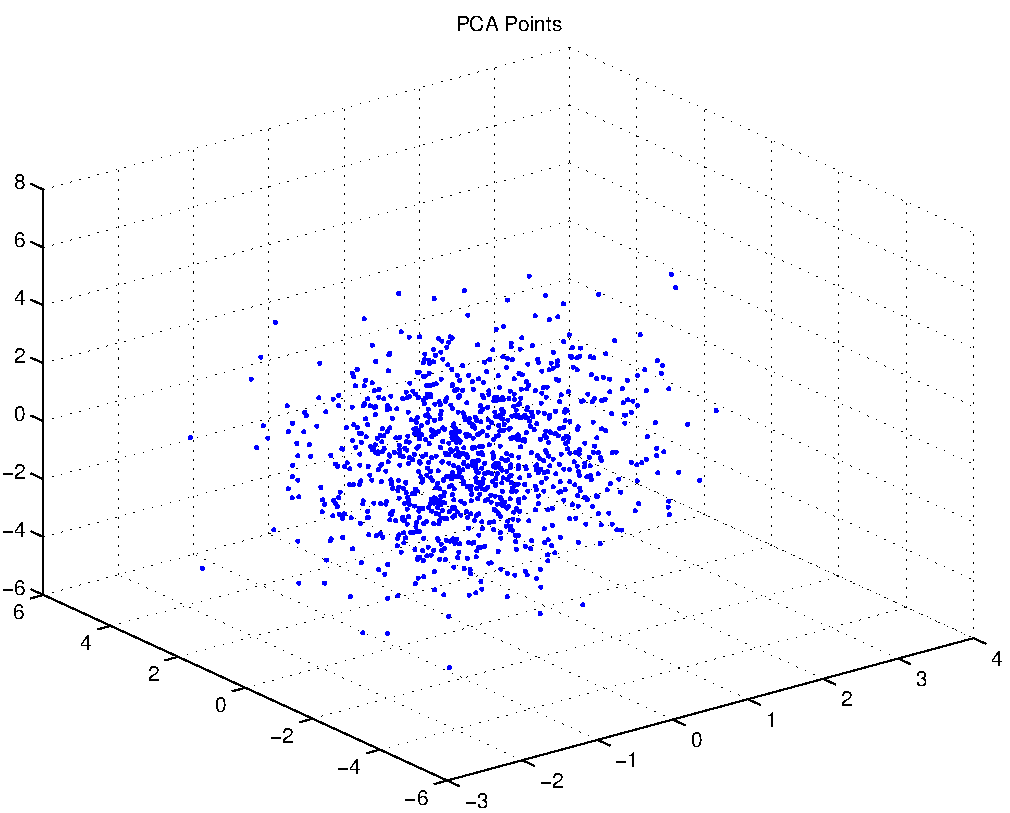
\includegraphics[width=10.0cm,height=10.0cm]{PCAPoints.pdf}

The eigenvectors:
+0.099, +0.246, +0.964
+0.166, +0.951, -0.259
-0.981, +0.186, +0.053

All of the eigenvalues of the covariance matrix:
(+0.958,+0.000), (+2.025,+0.000), (+3.017,+0.000)

QueryPerformanceCounter  =  +1.171
\subsubsection{Multi Variate Random Number Generator }
Sample from $N(\mu,\Sigma)$
mean= -0.002, variance=+1.004, skewness=+0.006, kurtosis=+3.003
mean= -0.001, variance=+1.017, skewness=-0.005, kurtosis=+2.988
mean= -0.002, variance=+1.006, skewness=-0.016, kurtosis=+3.014
Covariance Matrix 
+1.004, +0.009, +0.003
+0.009, +1.017, -0.003
+0.003, -0.003, +1.006

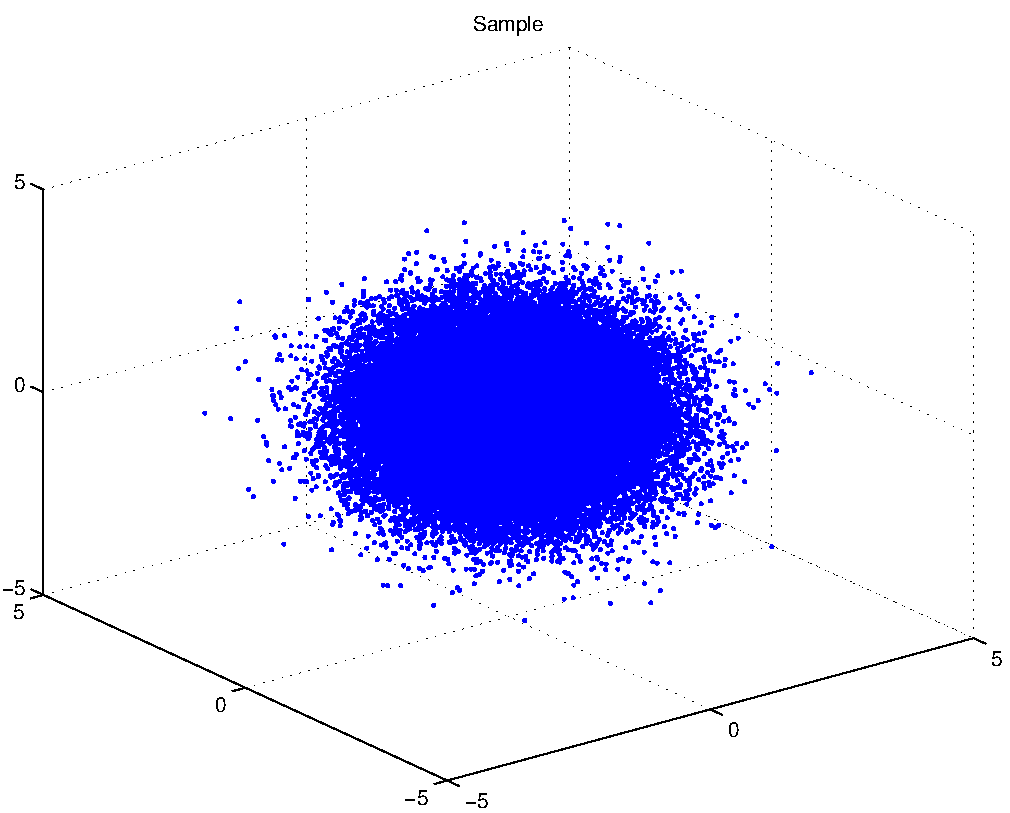
\includegraphics[width=10.0cm,height=10.0cm]{R_3_Normal.pdf}

Generate a sample from a unifom mixture of three Gaussians in $R^3$
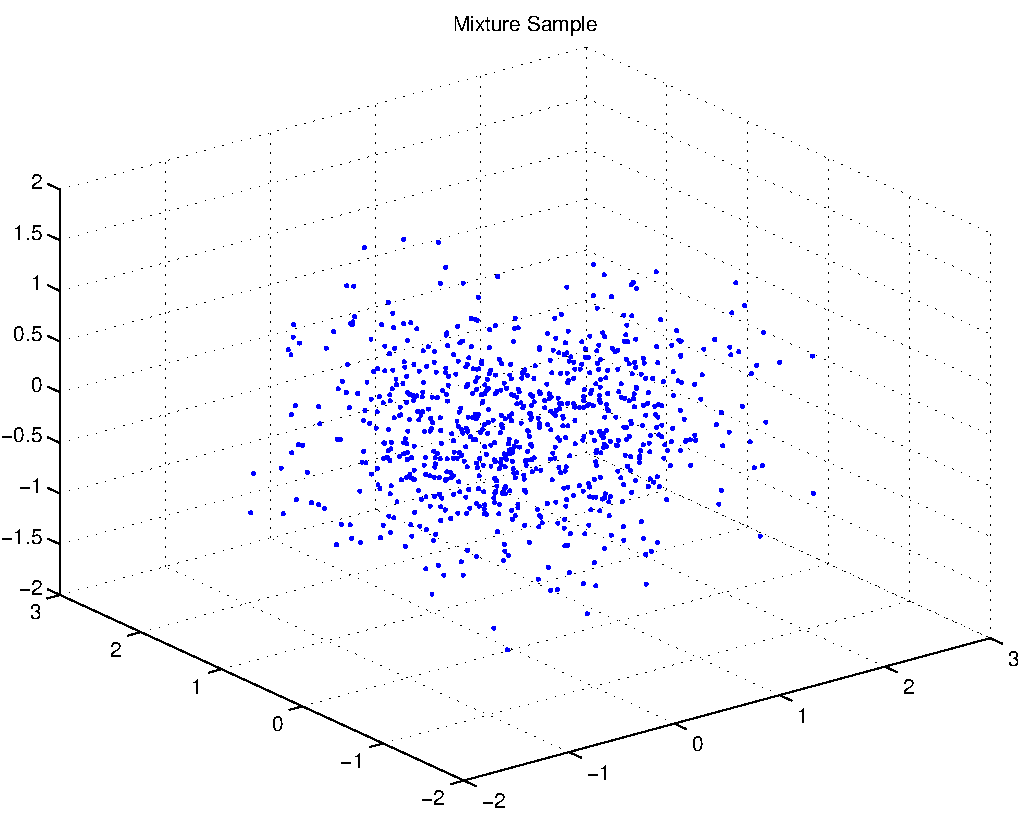
\includegraphics[width=10.0cm,height=10.0cm]{R_3_Normal_Mixture.pdf}

QueryPerformanceCounter  =  +17.063
\subsubsection{Matrix Multiply}
Comparing naive matrix multiply verus Intel MKL dgemm for matrix of size +2048.
This is for type double (hence the d in dgemm).
Naive type double matrix multiply tic toc  =  +0.396
dgemm plus row to column major transpose operation tic toc  =  +0.358
Comparing naive matrix multiply verus Intel MKL sgemm for matrix of size +2048.
This is for type float (hence the s in dgemm).
Naive type float matrix multiply tic toc  =  +0.238
sgemm plus row to column major transpose operation tic toc  =  +0.212
QueryPerformanceCounter  =  +1.343
\subsubsection{Descriptive Statistics}
Mean N(0,1): +0.003
Variance N(0,1): +1.006
Mean N(0,1) [recurrence relation method] :+0.003
Variance [recurrence relation method] :+1.006
Skewness : +0.007
Kurtosis : +2.997
QueryPerformanceCounter  =  +0.035
\subsubsection{Time Series }
+0.093
+0.726
+0.011
+2.178
QueryPerformanceCounter  =  +0.040
QueryPerformanceCounter  =  +6.725
\subsubsection{Iterated Exponential Filtering }
$\mu_1 =+0.093$
$\mu_2 =+0.726$
$\mu_3 =+0.011$
$\mu_4 =+2.178$
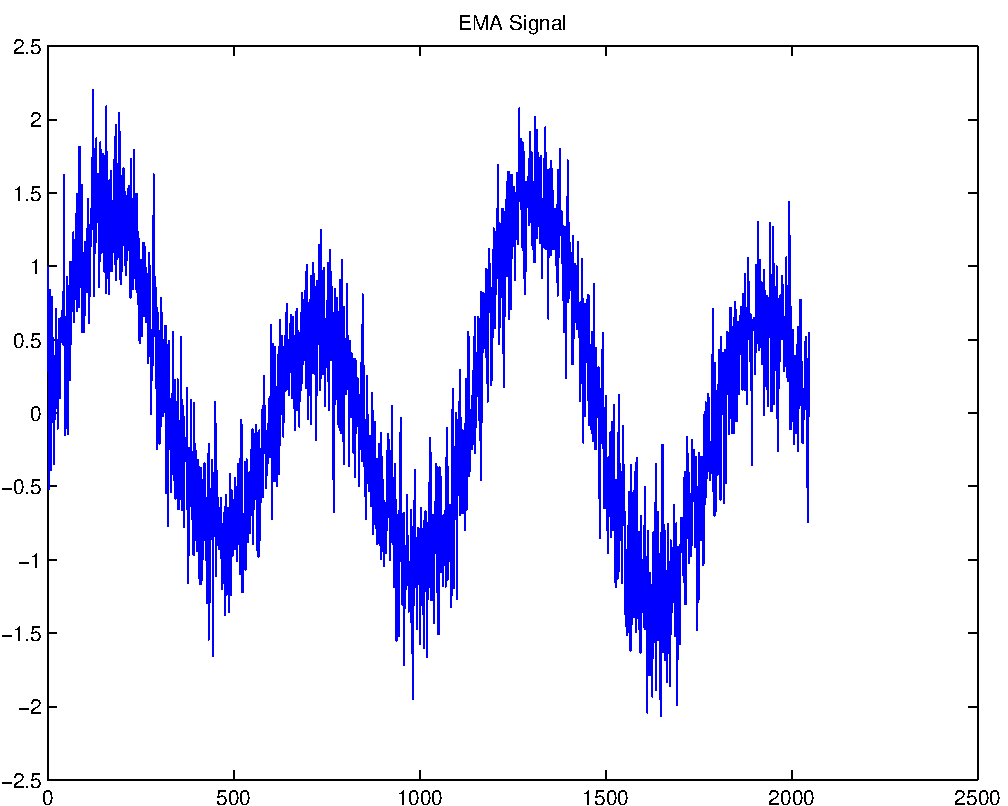
\includegraphics[width=10.0cm,height=10.0cm]{EMA_signal.pdf}

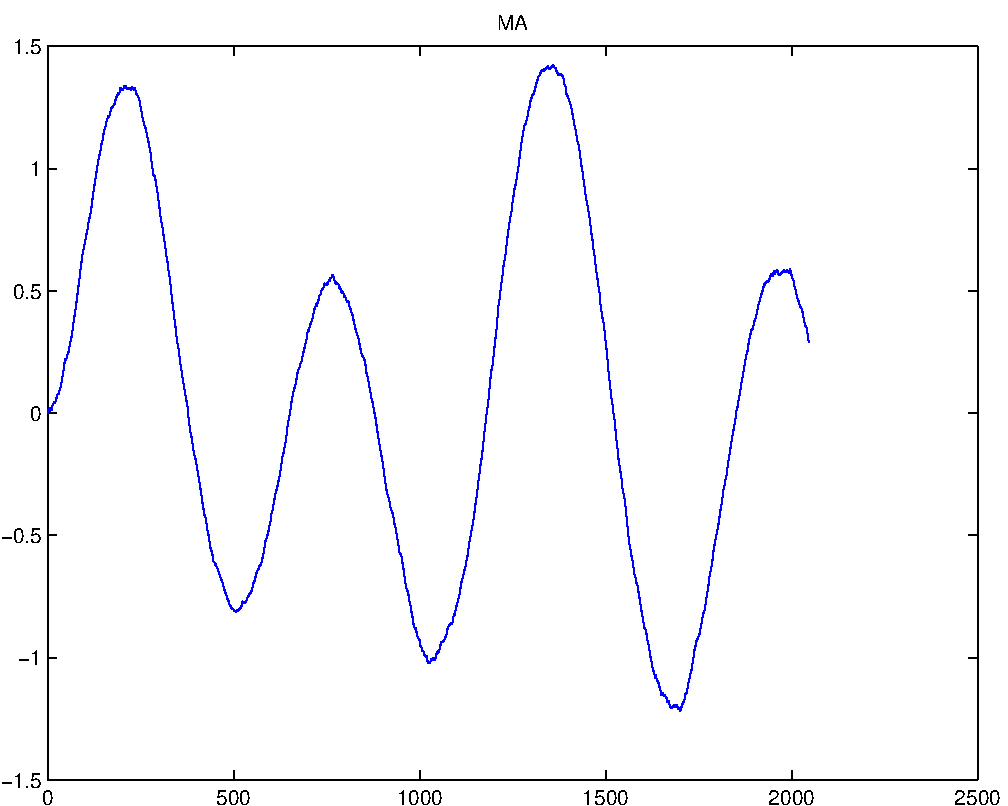
\includegraphics[width=10.0cm,height=10.0cm]{MA.pdf}

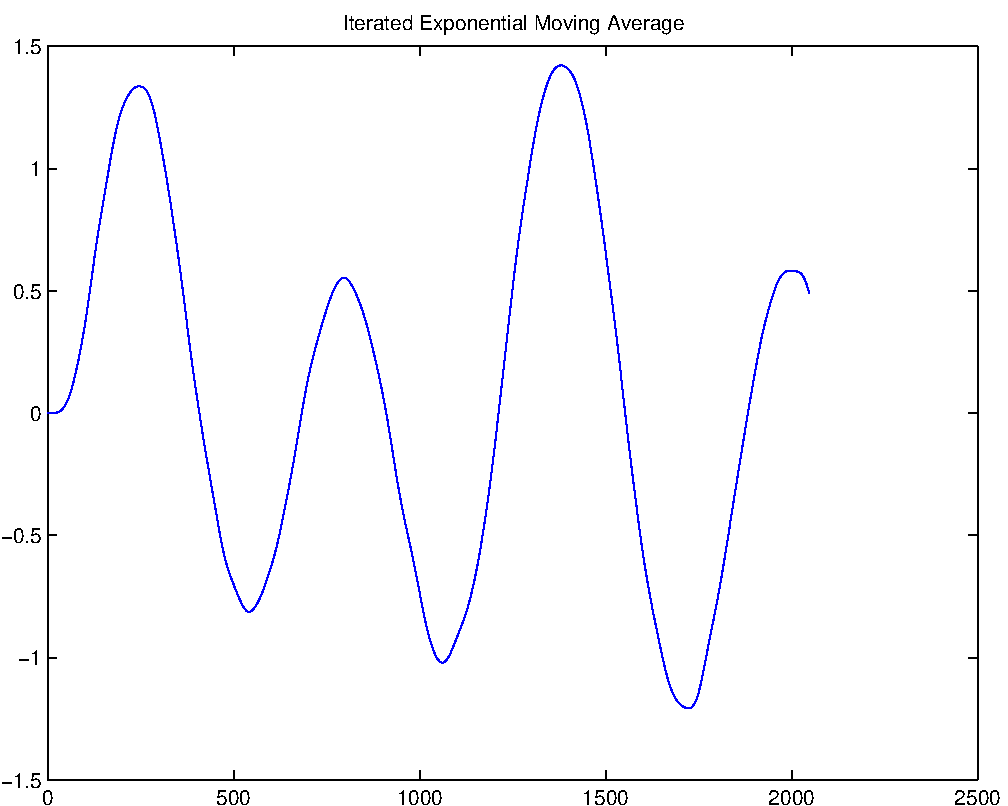
\includegraphics[width=10.0cm,height=10.0cm]{IEMA.pdf}

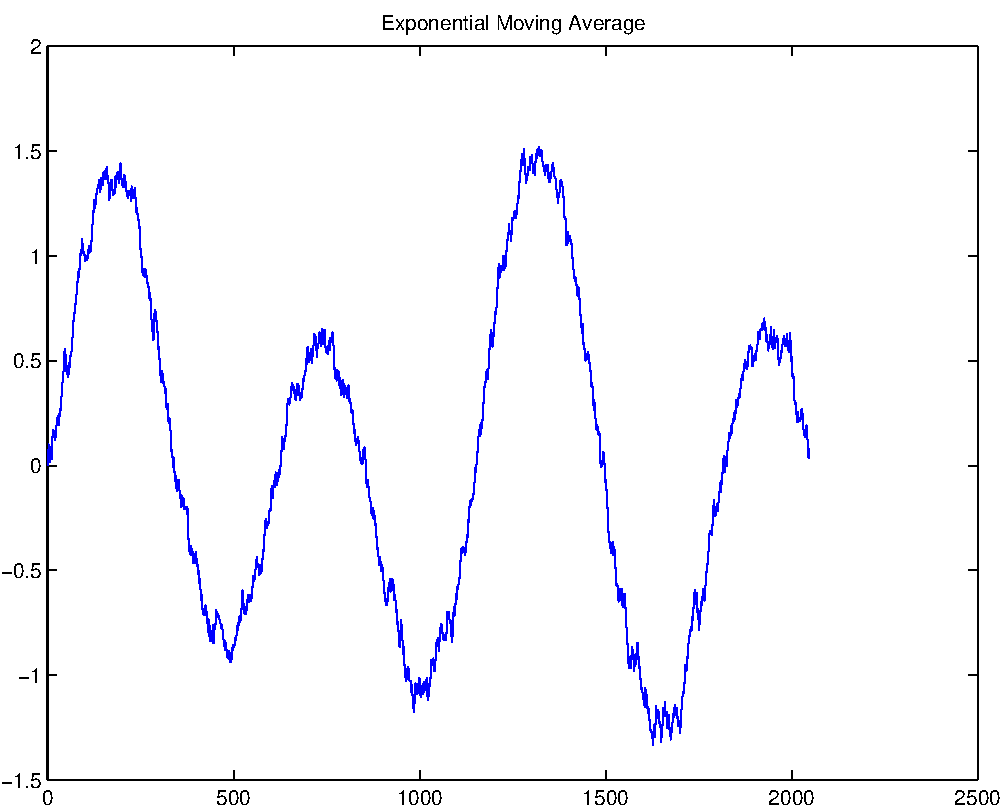
\includegraphics[width=10.0cm,height=10.0cm]{EMA.pdf}

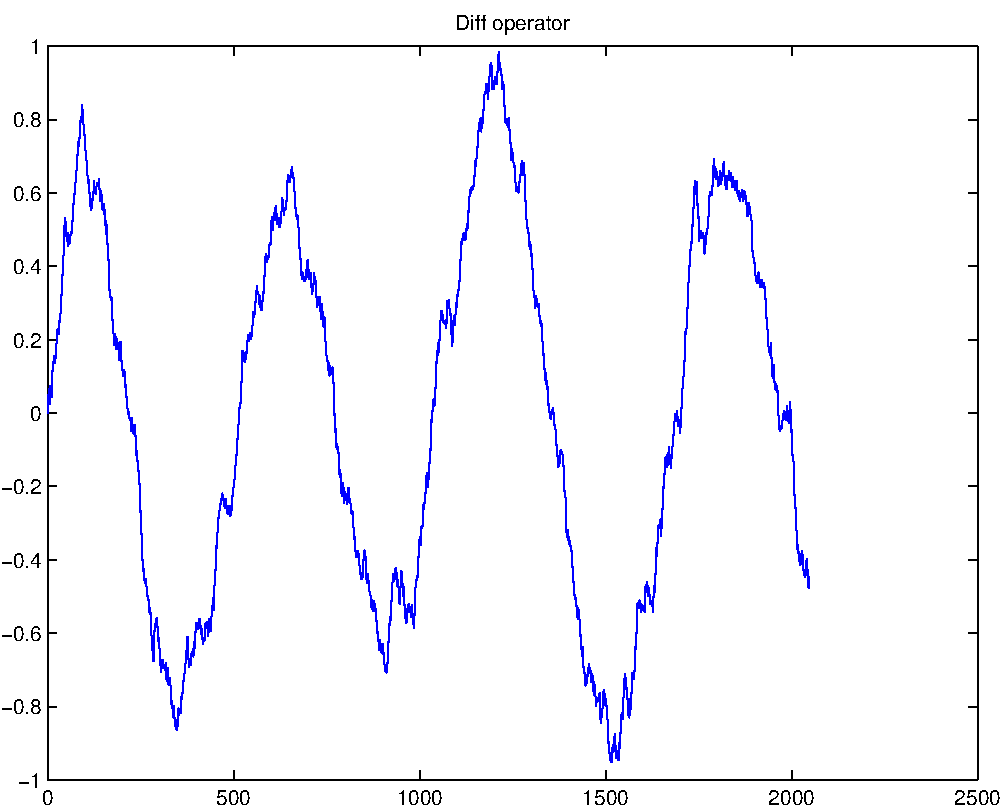
\includegraphics[width=10.0cm,height=10.0cm]{DIFF.pdf}

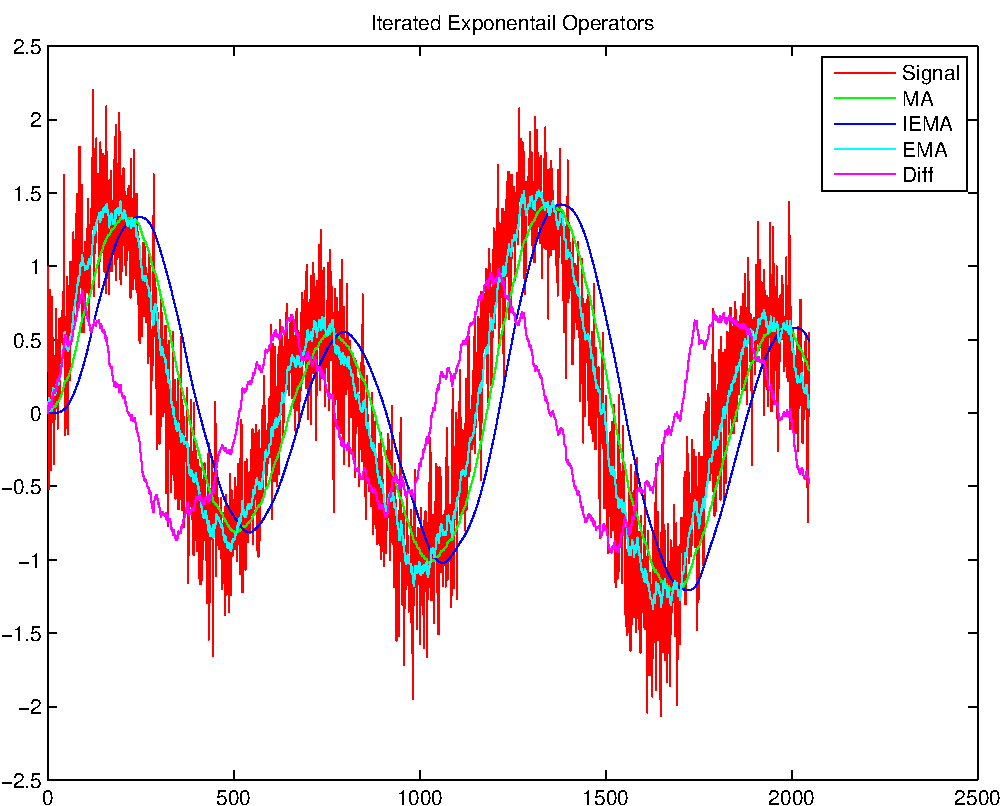
\includegraphics[width=10.0cm,height=10.0cm]{IteratedExponentailOperators.pdf}

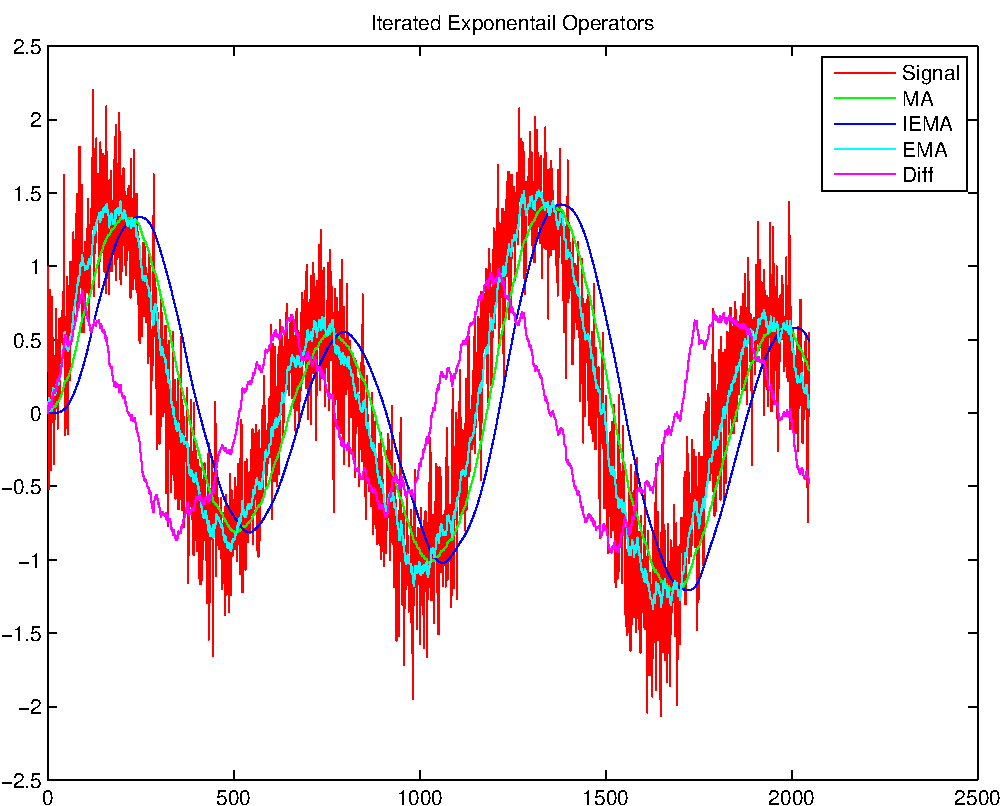
\includegraphics[width=10.0cm,height=10.0cm]{IteratedExponentailOperators.pdf}

QueryPerformanceCounter  =  +7.661
\subsubsection{Testing binary writer}
Binary writer Speedup 1GB Double Matrix +43.007

Binary reader Speedup 1GB Double Matrix +152.077

Binary writer Speedup 1GB Double vector +8.880

Binary reader Speedup 1GB Double Matrix +264.110

QueryPerformanceCounter  =  +0.734
\subsubsection{Testing Gaussian Mixture Point Cloud and Latex Plotting Capabilities.}
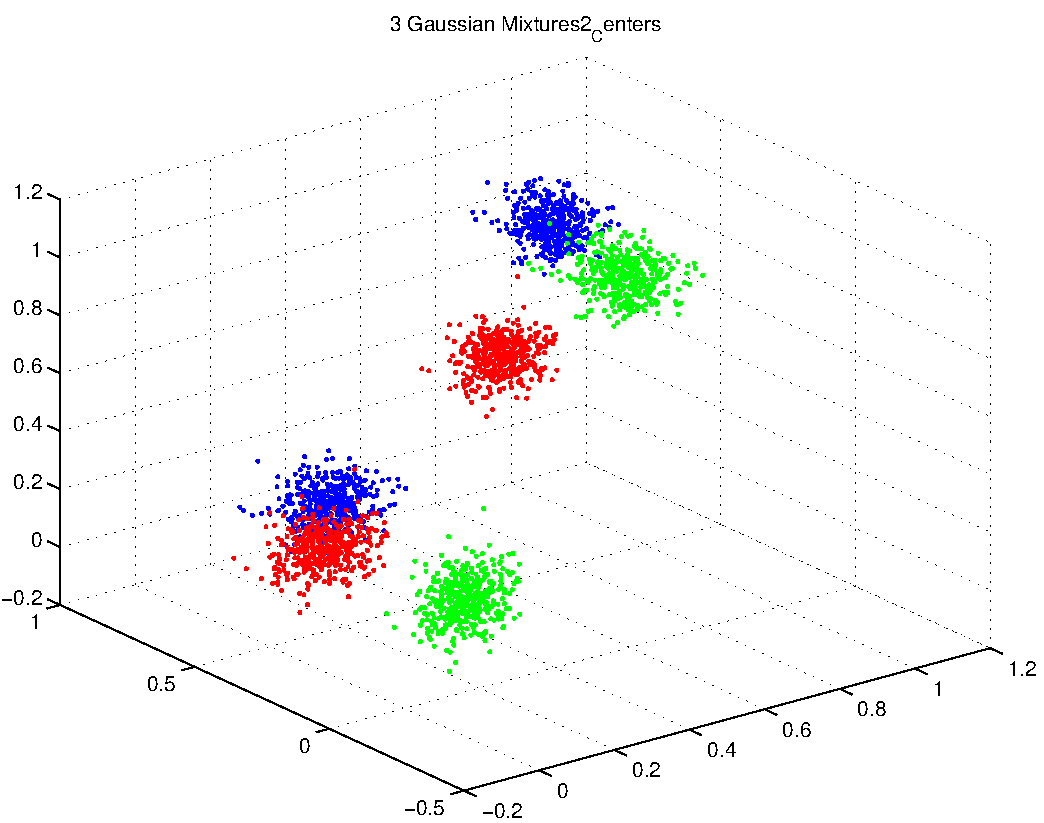
\includegraphics[width=10.0cm,height=10.0cm]{GaussianMixture_Dim_3_Centers2.pdf}

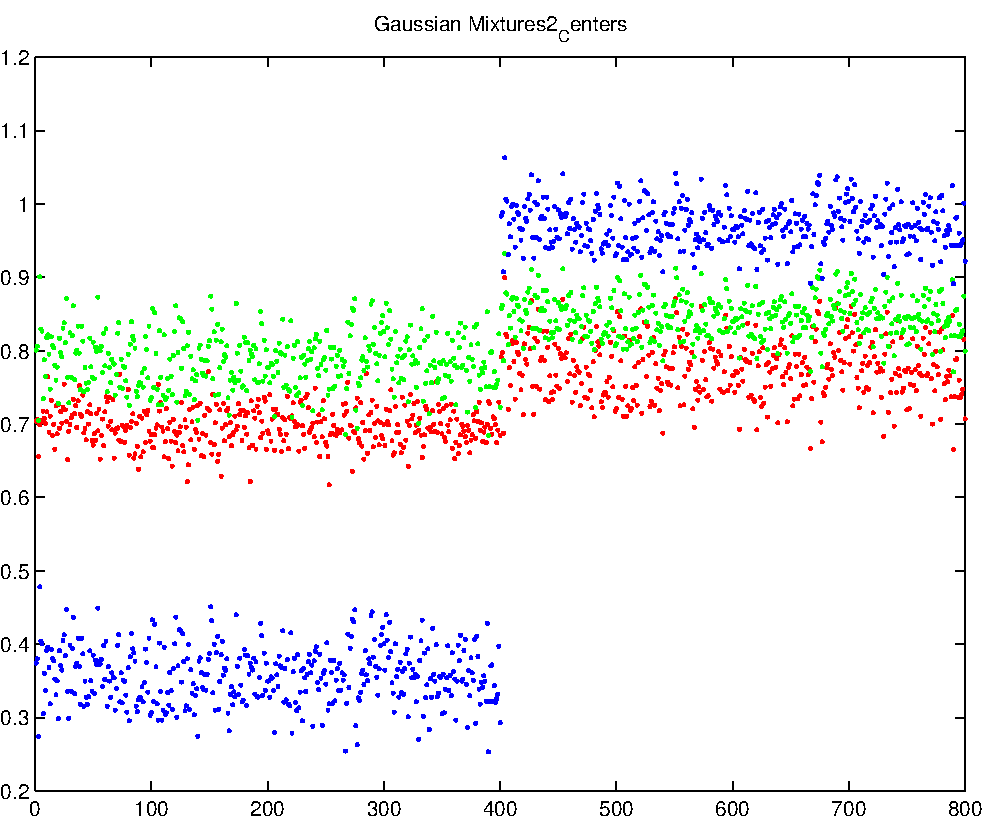
\includegraphics[width=10.0cm,height=10.0cm]{GaussianMixture_Dim_1_Centers2.pdf}

QueryPerformanceCounter  =  +2.843
\subsubsection{Intel VSL Function Check}
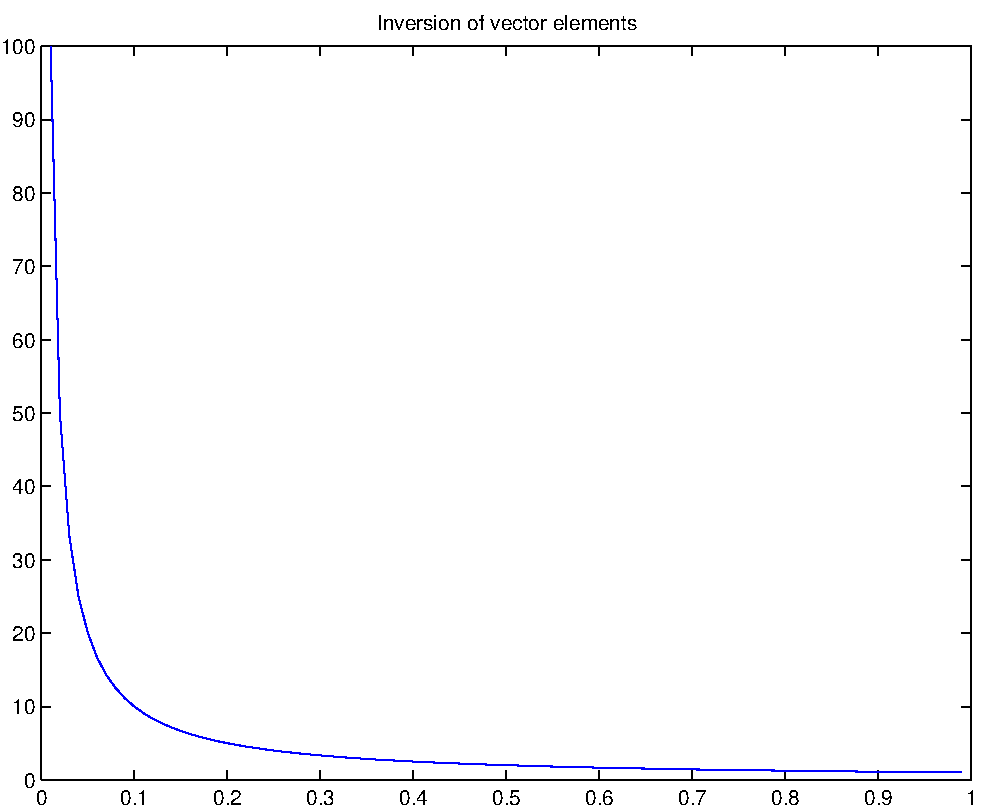
\includegraphics[width=10.0cm,height=10.0cm]{klVSLInv.pdf}

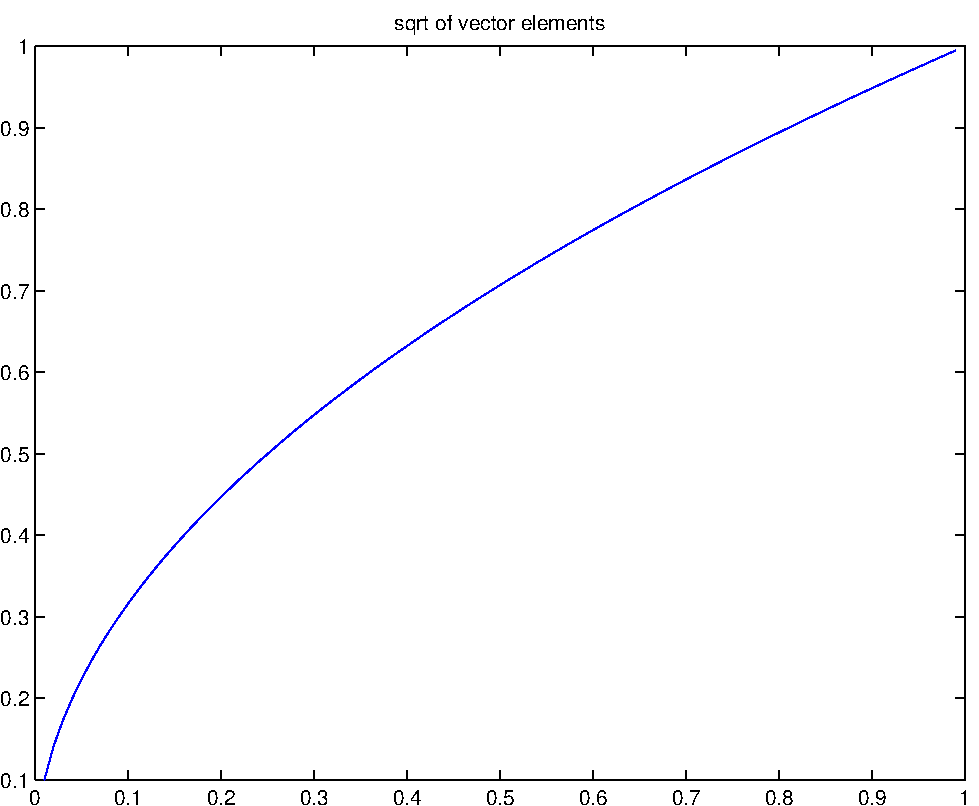
\includegraphics[width=10.0cm,height=10.0cm]{klVSLSqrt.pdf}

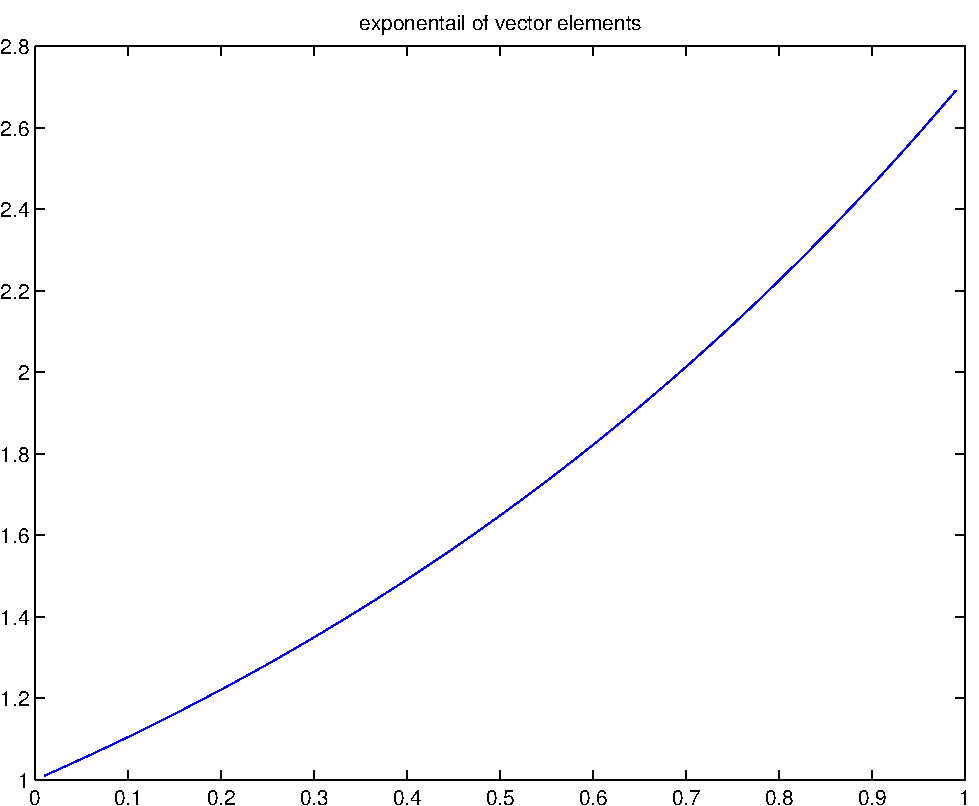
\includegraphics[width=10.0cm,height=10.0cm]{klVSLExp.pdf}

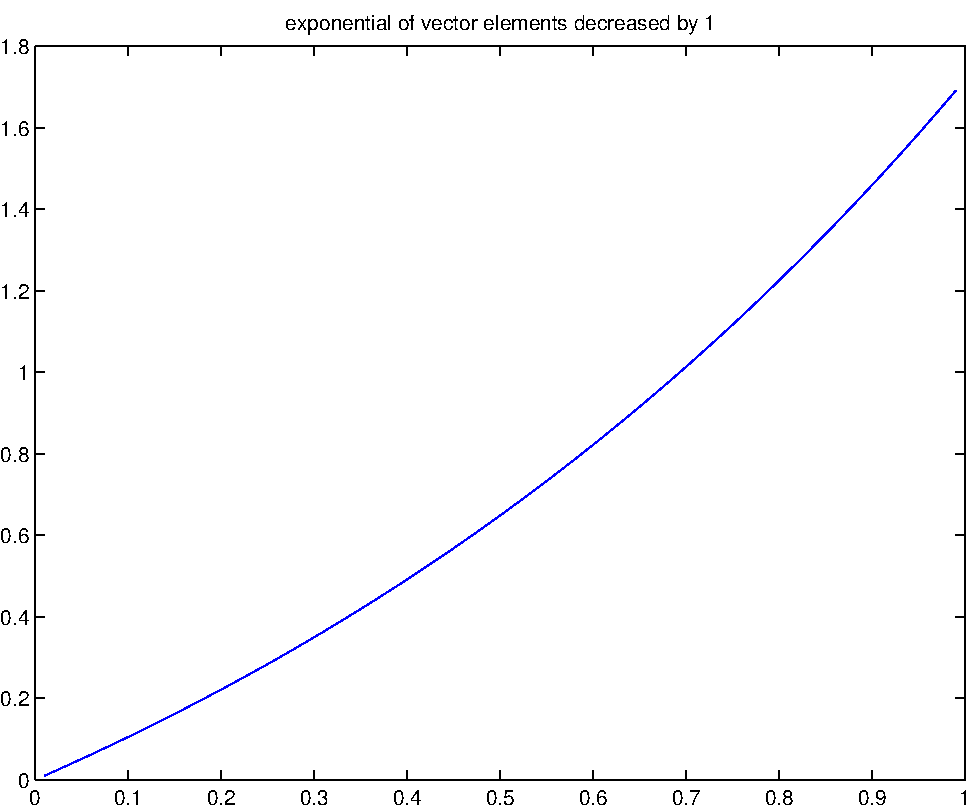
\includegraphics[width=10.0cm,height=10.0cm]{klVSLExpm1.pdf}

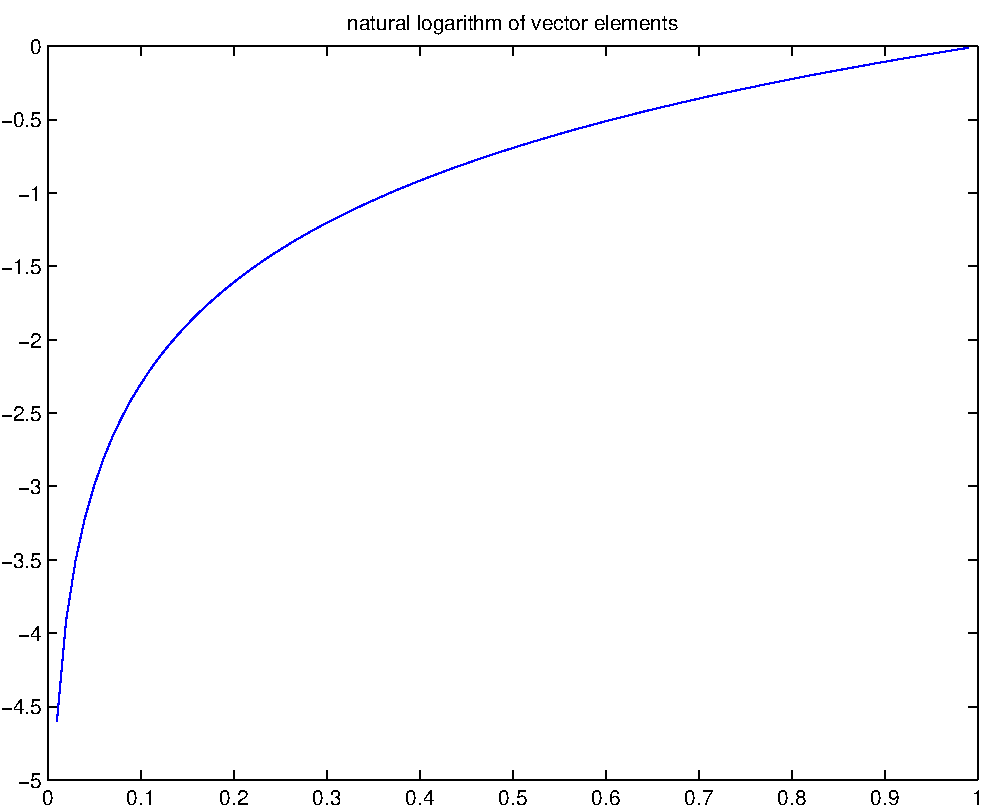
\includegraphics[width=10.0cm,height=10.0cm]{klVSLLn.pdf}

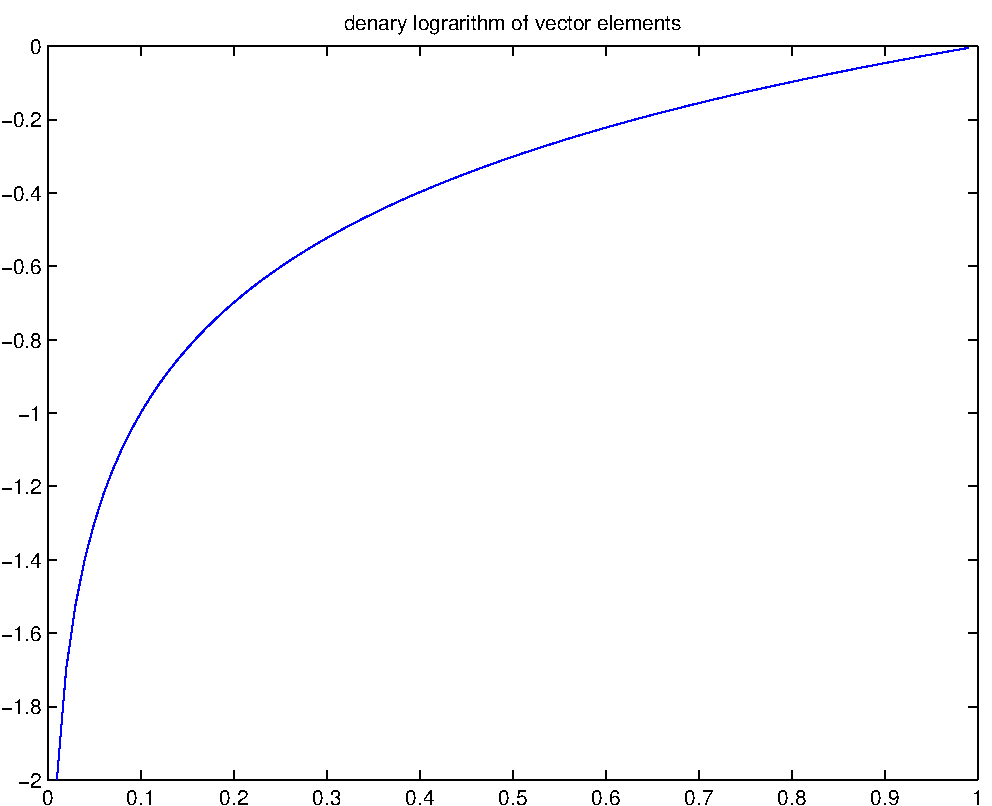
\includegraphics[width=10.0cm,height=10.0cm]{klVSLLog10.pdf}

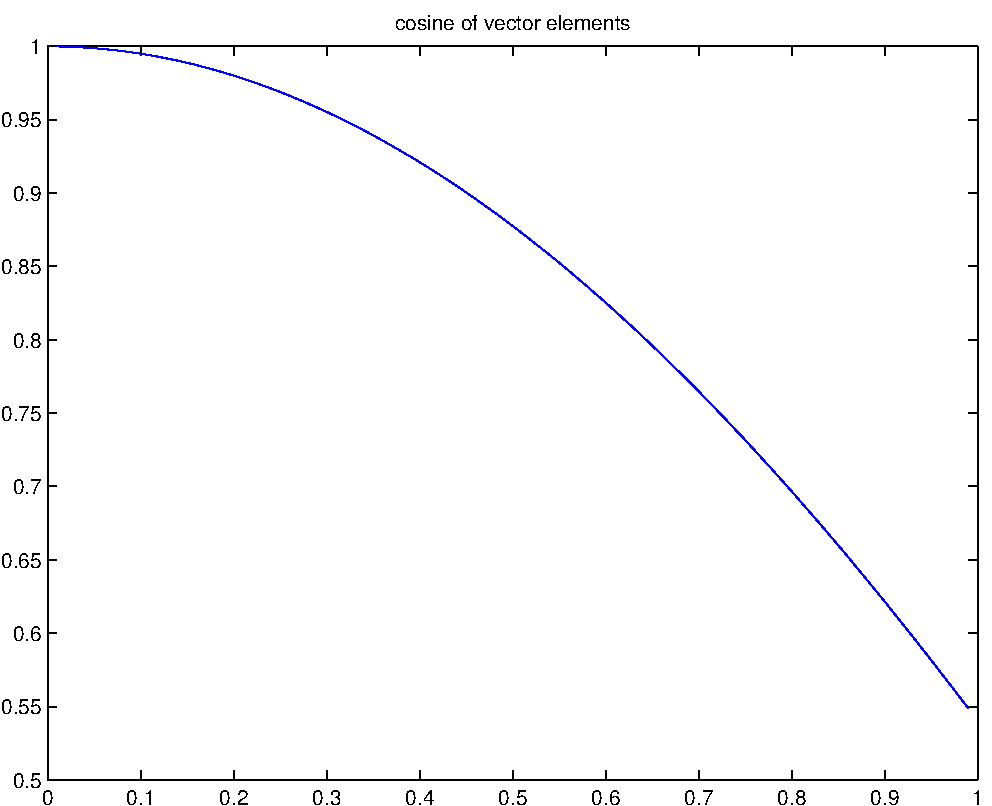
\includegraphics[width=10.0cm,height=10.0cm]{klVSLCos.pdf}

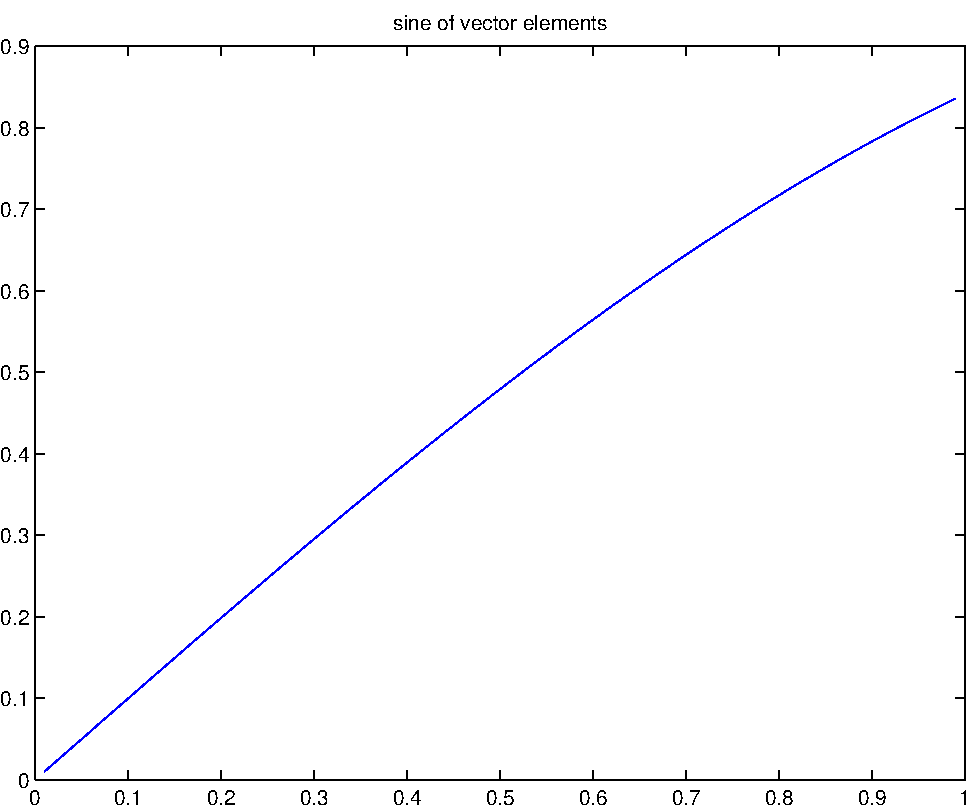
\includegraphics[width=10.0cm,height=10.0cm]{klVSLSin.pdf}

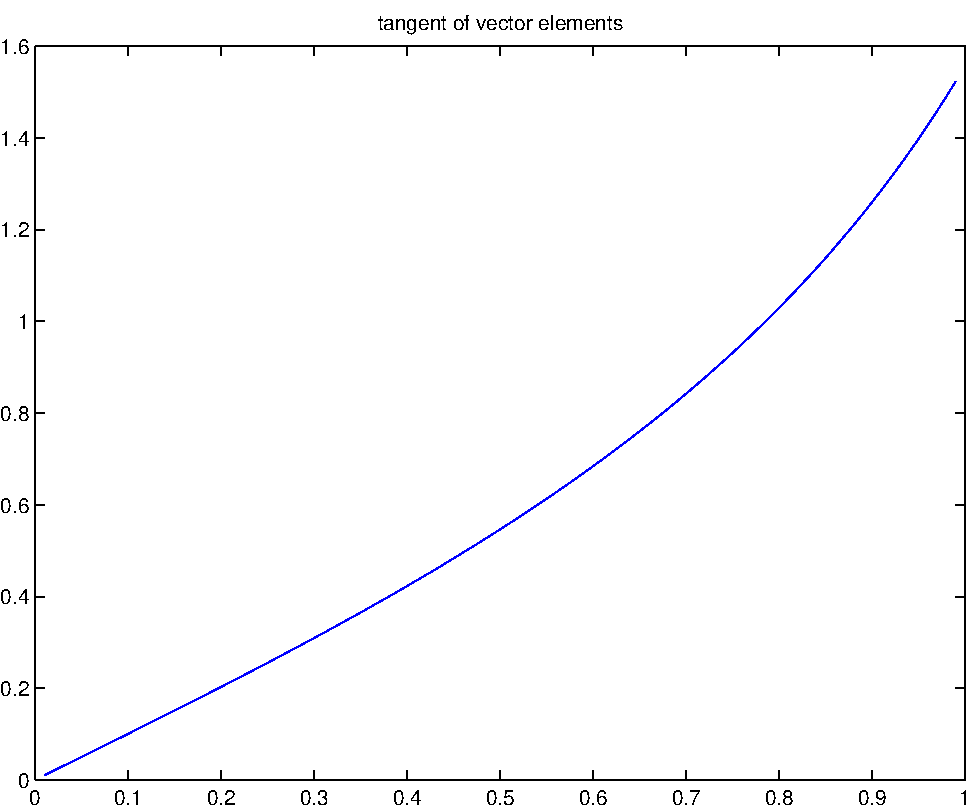
\includegraphics[width=10.0cm,height=10.0cm]{klVSLTan.pdf}

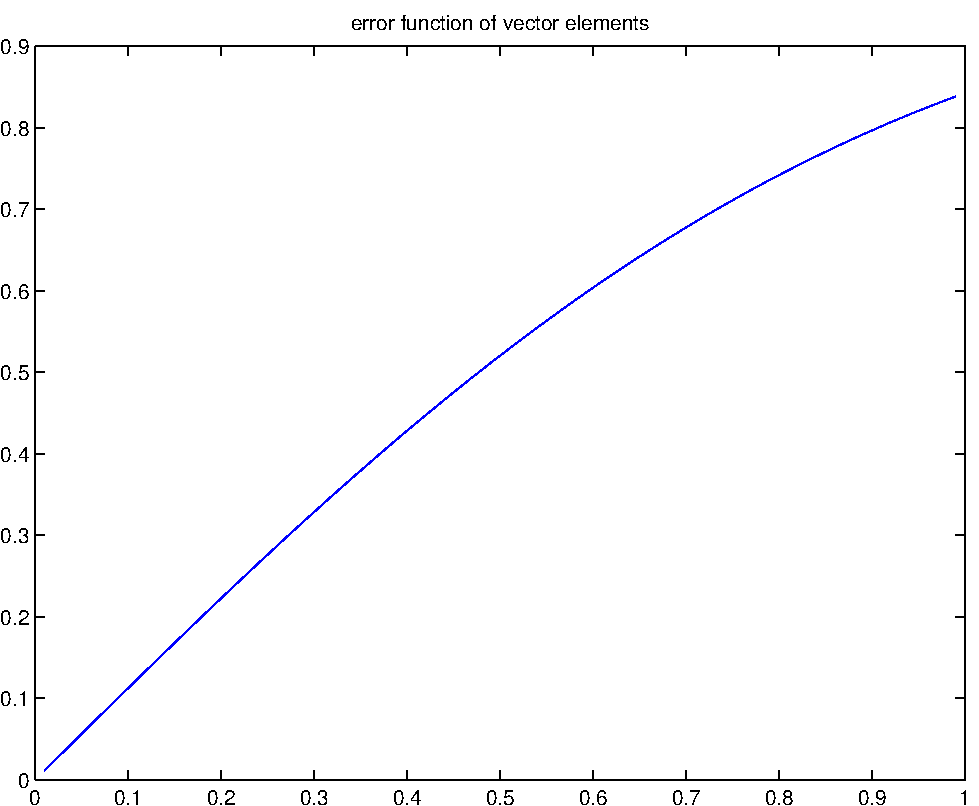
\includegraphics[width=10.0cm,height=10.0cm]{klVSLErf.pdf}

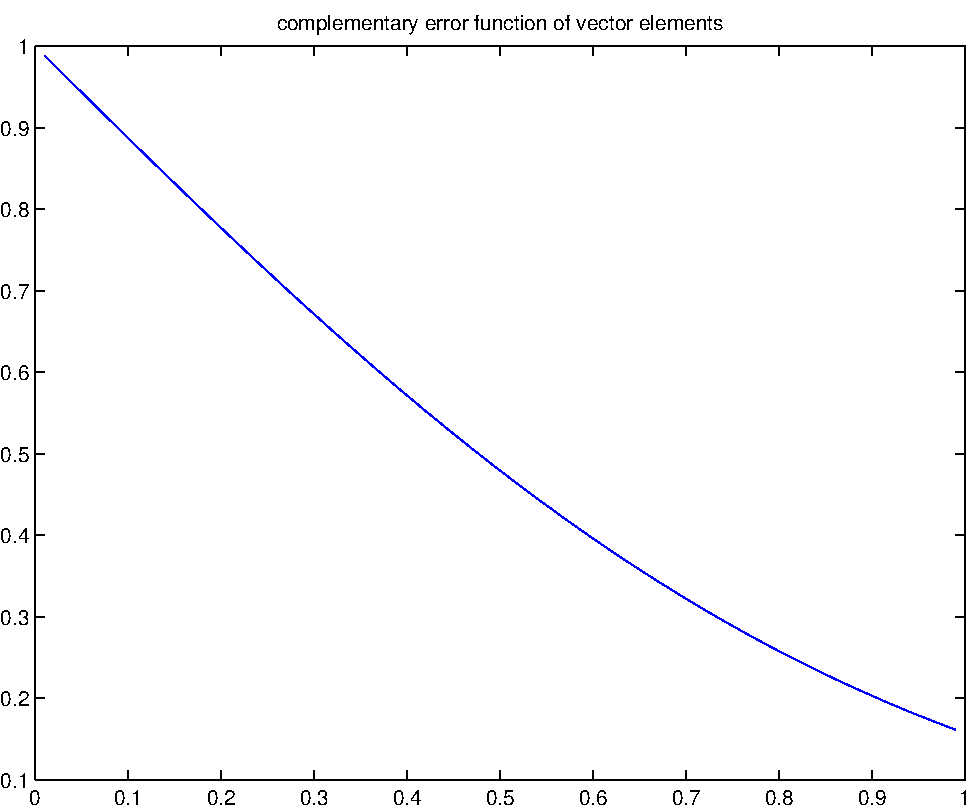
\includegraphics[width=10.0cm,height=10.0cm]{klVSLErfc.pdf}

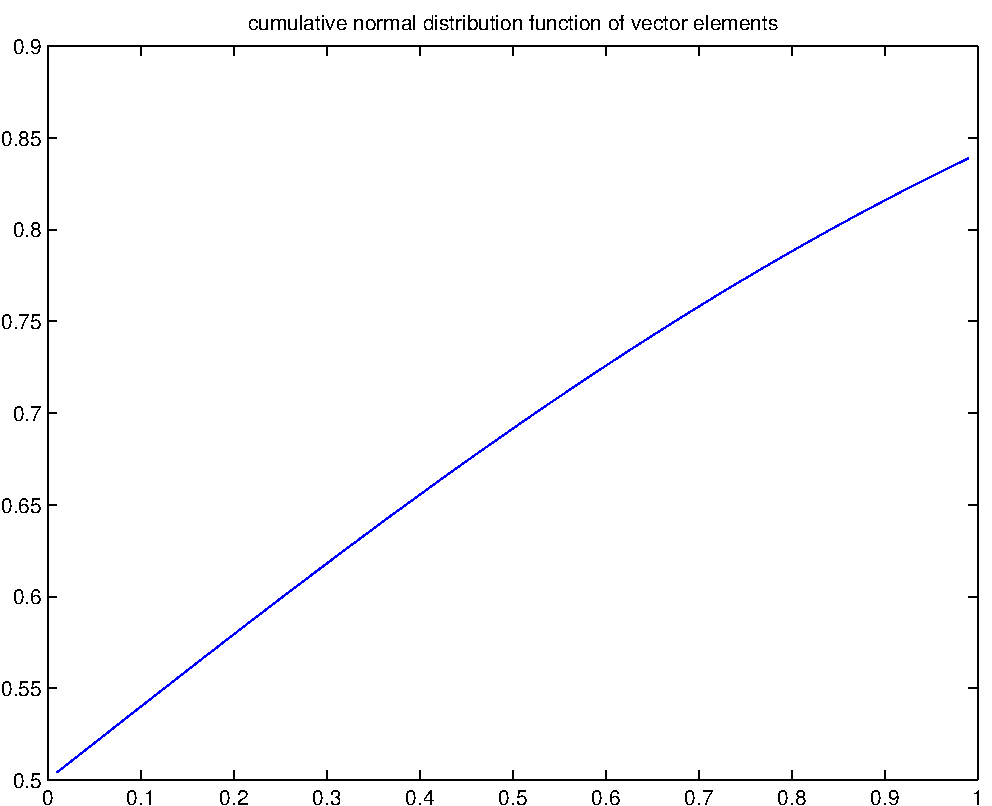
\includegraphics[width=10.0cm,height=10.0cm]{klVSLCdfNorm.pdf}

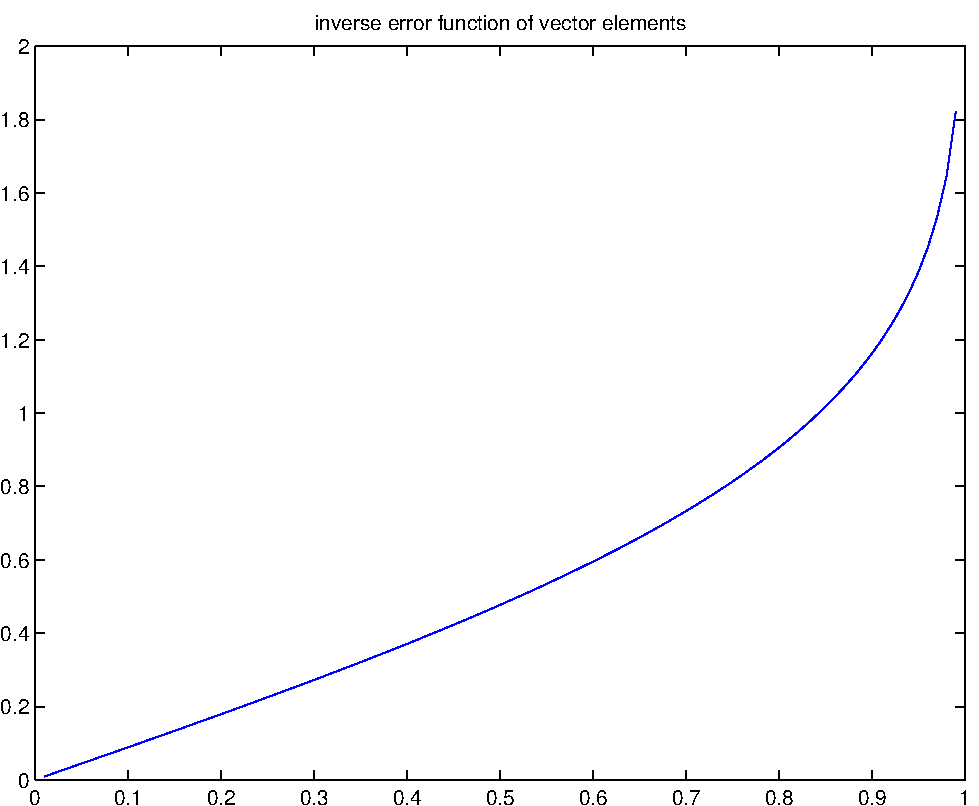
\includegraphics[width=10.0cm,height=10.0cm]{klVSLErfInv.pdf}

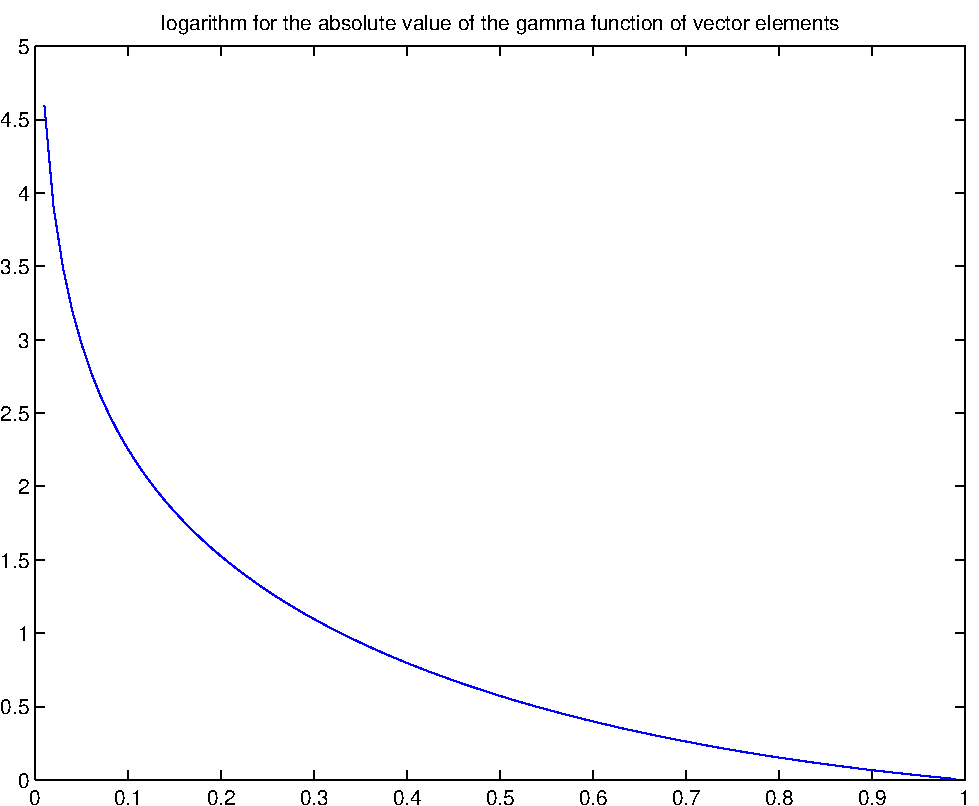
\includegraphics[width=10.0cm,height=10.0cm]{klVSLLGamma.pdf}

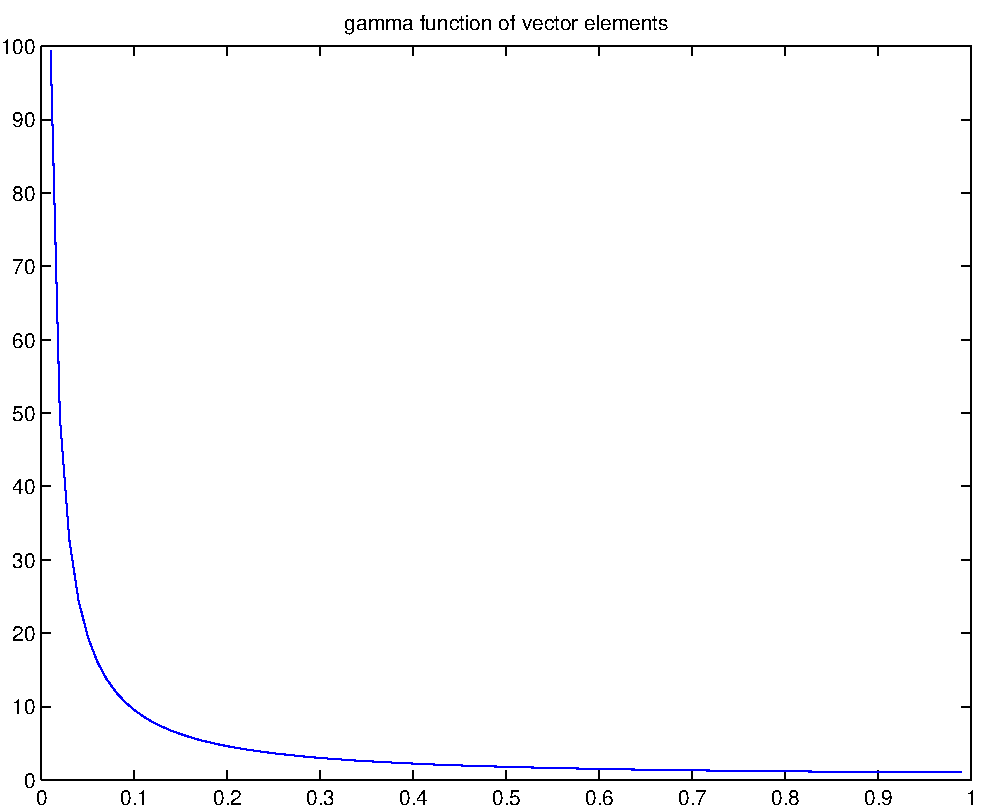
\includegraphics[width=10.0cm,height=10.0cm]{klVSLTGamma.pdf}

QueryPerformanceCounter  =  +14.779
\subsubsection{Gram Matrix Consistency Check}
Sample Size = 4096
Feature dim = 3

$$Sigma$ = \left(
\begin{array}{
ccc}
+1.140 & +1.535 & +0.581 \\
+1.535 & +9.988 & +1.605 \\
+0.581 & +1.605 & +0.428 \\
\end{array}
\right)$ \newline 

$Sample Covariance = \left(
\begin{array}{
ccc}
+1.123 & +1.485 & +0.577 \\
+1.485 & +10.013 & +1.603 \\
+0.577 & +1.603 & +0.431 \\
\end{array}
\right)$ \newline 

$Sample Mean = \left(
\begin{array}{
ccc}
+1.02663 & +1.02396 & +1.01467 \\
\end{array}
\right)$ \newline 

$Sample Covariance-$Omega$ = \left(
\begin{array}{
ccc}
-0.017 & -0.050 & -0.004 \\
-0.050 & +0.025 & -0.002 \\
-0.004 & -0.002 & +0.004 \\
\end{array}
\right)$ \newline 

$Sample Covariance Eigs = \left(
\begin{array}{
ccc}
(+10.53249,+0.00000) & (+0.99425,+0.00000) & (+0.04081,+0.00000) \\
\end{array}
\right)$ \newline 

$Centered Mean = \left(
\begin{array}{
ccc}
-0.00000 & +0.00000 & -0.00000 \\
\end{array}
\right)$ \newline 

$Centered Covariance = \left(
\begin{array}{
ccc}
+1.123 & +1.485 & +0.577 \\
+1.485 & +10.013 & +1.603 \\
+0.577 & +1.603 & +0.431 \\
\end{array}
\right)$ \newline 

$Gram Matrix Gf Not scaled by sample size = \left(
\begin{array}{
ccc}
+4599.978 & +6080.618 & +2363.151 \\
+6080.618 & +41013.459 & +6564.233 \\
+2363.151 & +6564.233 & +1767.264 \\
\end{array}
\right)$ \newline 

$Gram Matrix Gf  scaled by sample size = \left(
\begin{array}{
ccc}
+1.123 & +1.485 & +0.577 \\
+1.485 & +10.013 & +1.603 \\
+0.577 & +1.603 & +0.431 \\
\end{array}
\right)$ \newline 

$SampleCovariance - Scaled Gf = \left(
\begin{array}{
ccc}
+0.000 & +0.000 & +0.000 \\
+0.000 & +0.002 & +0.000 \\
+0.000 & +0.000 & +0.000 \\
\end{array}
\right)$ \newline 

$EigenDecomp of SampleCovariance = \left(
\begin{array}{
ccc}
-0.164 & -0.973 & -0.164 \\
+0.917 & -0.211 & +0.339 \\
-0.364 & -0.095 & +0.927 \\
\end{array}
\right)$ \newline 

$EigenDecomp of Gram Matrix = \left(
\begin{array}{
ccc}
-0.107 & -0.977 & -0.185 \\
-0.278 & +0.209 & -0.938 \\
+0.955 & -0.049 & -0.294 \\
\end{array}
\right)$ \newline 

QueryPerformanceCounter  =  +1.384
\subsubsection{Eigen Solver Checks}
\subsubsection{Haar Distributed Random Orthogonal Matrix $A \in O(n)$}
 Testing Operator Norm
Number of Dimensions: +8

$A = \left(
\begin{array}{
cccccccc}
-0.177 & -0.049 & -0.053 & -0.078 & +0.637 & -0.523 & +0.357 & -0.389 \\
-0.410 & -0.184 & +0.147 & -0.041 & +0.409 & -0.121 & -0.414 & +0.650 \\
-0.066 & -0.447 & -0.263 & +0.767 & +0.009 & -0.019 & -0.278 & -0.246 \\
-0.510 & -0.466 & -0.175 & -0.145 & -0.449 & -0.074 & +0.489 & +0.157 \\
+0.263 & -0.694 & +0.353 & -0.363 & +0.170 & +0.317 & -0.088 & -0.237 \\
-0.376 & +0.155 & +0.819 & +0.298 & -0.148 & +0.016 & +0.073 & -0.218 \\
+0.062 & +0.041 & -0.012 & +0.328 & +0.398 & +0.580 & +0.557 & +0.286 \\
-0.568 & +0.199 & -0.283 & -0.235 & +0.129 & +0.518 & -0.249 & -0.395 \\
\end{array}
\right)$ \newline 

$Det(A) :   A \in O(n)$ = (+1.000,+0.000)

$L = \left(
\begin{array}{
cccccccc}
+1.000 & +0.000 & +0.000 & +0.000 & +0.000 & +0.000 & +0.000 & +0.000 \\
+0.898 & +1.000 & +0.000 & +0.000 & +0.000 & +0.000 & +0.000 & +0.000 \\
+0.663 & -0.036 & +1.000 & +0.000 & +0.000 & +0.000 & +0.000 & +0.000 \\
+0.115 & +0.729 & -0.285 & +1.000 & +0.000 & +0.000 & +0.000 & +0.000 \\
-0.463 & +0.933 & +0.147 & -0.686 & +1.000 & +0.000 & +0.000 & +0.000 \\
+0.312 & +0.172 & +0.021 & -0.029 & +0.694 & +1.000 & +0.000 & +0.000 \\
-0.109 & -0.097 & -0.035 & +0.370 & +0.220 & -0.148 & +1.000 & +0.000 \\
+0.721 & +0.507 & +0.308 & -0.052 & +0.683 & +0.664 & -0.440 & +1.000 \\
\end{array}
\right)$ \newline 

$U = \left(
\begin{array}{
cccccccc}
-0.568 & +0.199 & -0.283 & -0.235 & +0.129 & +0.518 & -0.249 & -0.395 \\
+0.000 & -0.645 & +0.079 & +0.066 & -0.564 & -0.540 & +0.713 & +0.512 \\
+0.000 & +0.000 & +1.009 & +0.456 & -0.253 & -0.347 & +0.264 & +0.063 \\
+0.000 & +0.000 & +0.000 & +0.876 & +0.333 & +0.216 & -0.693 & -0.556 \\
+0.000 & +0.000 & +0.000 & +0.000 & +1.022 & +1.260 & -1.382 & -1.288 \\
+0.000 & +0.000 & +0.000 & +0.000 & +0.000 & -1.452 & +1.245 & +0.522 \\
+0.000 & +0.000 & +0.000 & +0.000 & +0.000 & +0.000 & +1.353 & +0.861 \\
+0.000 & +0.000 & +0.000 & +0.000 & +0.000 & +0.000 & +0.000 & +1.539 \\
\end{array}
\right)$ \newline 

$L * U  = \left(
\begin{array}{
cccccccc}
-0.568 & +0.199 & -0.283 & -0.235 & +0.129 & +0.518 & -0.249 & -0.395 \\
-0.510 & -0.466 & -0.175 & -0.145 & -0.449 & -0.074 & +0.489 & +0.157 \\
-0.376 & +0.155 & +0.819 & +0.298 & -0.148 & +0.016 & +0.073 & -0.218 \\
-0.066 & -0.447 & -0.263 & +0.767 & +0.009 & -0.019 & -0.278 & -0.246 \\
+0.263 & -0.694 & +0.353 & -0.363 & +0.170 & +0.317 & -0.088 & -0.237 \\
-0.177 & -0.049 & -0.053 & -0.078 & +0.637 & -0.523 & +0.357 & -0.389 \\
+0.062 & +0.041 & -0.012 & +0.328 & +0.398 & +0.580 & +0.557 & +0.286 \\
-0.410 & -0.184 & +0.147 & -0.041 & +0.409 & -0.121 & -0.414 & +0.650 \\
\end{array}
\right)$ \newline 

$Det(L) :    = (+1.000,+0.000)     Det(U) :    = (-1.000,+0.000)     Det(LU) :    = (-1.000,+0.000)$

$||A||_{L_1}$  = +2.577

$||A||_{L_{\infty}}$ = +2.575

$||A^{-1}||_{L_1}$  = +2.575

$||A^{-1}||_{L_{\infty}}$ = +2.577

$||A||_{L_{\infty}} * ||A^{-1}||_{L_{\infty}} = +6.636$

$||A||_{L_1} * ||A^{-1}||_{L_1} = +6.636$

Frobenious Norm  $||A||_{\textit{F}}$ via $\sum\limits_{i,j =0}^{n} \|A_{i,j}|$   of  $A \in O(n)$  +2.828

$L_1$ condition number of Haar Distributed Random Orthogonal Matrix $A \in O(n)$ +5.421

$A = \left(
\begin{array}{
cccccccc}
-0.177 & -0.049 & -0.053 & -0.078 & +0.637 & -0.523 & +0.357 & -0.389 \\
-0.410 & -0.184 & +0.147 & -0.041 & +0.409 & -0.121 & -0.414 & +0.650 \\
-0.066 & -0.447 & -0.263 & +0.767 & +0.009 & -0.019 & -0.278 & -0.246 \\
-0.510 & -0.466 & -0.175 & -0.145 & -0.449 & -0.074 & +0.489 & +0.157 \\
+0.263 & -0.694 & +0.353 & -0.363 & +0.170 & +0.317 & -0.088 & -0.237 \\
-0.376 & +0.155 & +0.819 & +0.298 & -0.148 & +0.016 & +0.073 & -0.218 \\
+0.062 & +0.041 & -0.012 & +0.328 & +0.398 & +0.580 & +0.557 & +0.286 \\
-0.568 & +0.199 & -0.283 & -0.235 & +0.129 & +0.518 & -0.249 & -0.395 \\
\end{array}
\right)$ \newline 

$L_{\infty}$ condition number of Haar Distributed Random Orthogonal Matrix $A \in O(n)$ +6.636

Eigenvalues of $A \in O(n)$

(+0.347,+0.938), (+0.347,-0.938), (-0.543,+0.839), (-0.543,-0.839), (-0.990,+0.144), (-0.990,-0.144), (+0.976,+0.218), (+0.976,-0.218)

 $|\lambda | : \lambda \in \sigma(A) , A \in O(n)$

+1.000, +1.000, +1.000, +1.000, +1.000, +1.000, +1.000, +1.000


Calculating $A^{\dag} A,$  we expect $A^{\dag} A \approx I$

$A^{\dag} A = \left(
\begin{array}{
cccccccc}
+1.000 & -0.000 & +0.000 & -0.000 & +0.000 & +0.000 & +0.000 & +0.000 \\
-0.000 & +1.000 & +0.000 & +0.000 & +0.000 & -0.000 & -0.000 & +0.000 \\
+0.000 & +0.000 & +1.000 & +0.000 & -0.000 & +0.000 & -0.000 & +0.000 \\
-0.000 & +0.000 & +0.000 & +1.000 & +0.000 & +0.000 & +0.000 & +0.000 \\
+0.000 & +0.000 & -0.000 & +0.000 & +1.000 & +0.000 & +0.000 & +0.000 \\
+0.000 & -0.000 & +0.000 & +0.000 & +0.000 & +1.000 & +0.000 & +0.000 \\
+0.000 & -0.000 & -0.000 & +0.000 & +0.000 & +0.000 & +1.000 & +0.000 \\
+0.000 & +0.000 & +0.000 & +0.000 & +0.000 & +0.000 & +0.000 & +1.000 \\
\end{array}
\right)$ \newline 

Calculating $A^{-1} ,  A \in O(n)$.

$A^{-1} = \left(
\begin{array}{
cccccccc}
-0.177 & -0.410 & -0.066 & -0.510 & +0.263 & -0.376 & +0.062 & -0.568 \\
-0.049 & -0.184 & -0.447 & -0.466 & -0.694 & +0.155 & +0.041 & +0.199 \\
-0.053 & +0.147 & -0.263 & -0.175 & +0.353 & +0.819 & -0.012 & -0.283 \\
-0.078 & -0.041 & +0.767 & -0.145 & -0.363 & +0.298 & +0.328 & -0.235 \\
+0.637 & +0.409 & +0.009 & -0.449 & +0.170 & -0.148 & +0.398 & +0.129 \\
-0.523 & -0.121 & -0.019 & -0.074 & +0.317 & +0.016 & +0.580 & +0.518 \\
+0.357 & -0.414 & -0.278 & +0.489 & -0.088 & +0.073 & +0.557 & -0.249 \\
-0.389 & +0.650 & -0.246 & +0.157 & -0.237 & -0.218 & +0.286 & -0.395 \\
\end{array}
\right)$ \newline 

Calculating $A^{-1} *A  ,  A \in O(n)$.   We expect $A^{-1} *A  \approx I$. 

$A^{-1} *A = \left(
\begin{array}{
cccccccc}
+1.000 & -0.000 & +0.000 & +0.000 & -0.000 & -0.000 & -0.000 & +0.000 \\
+0.000 & +1.000 & -0.000 & +0.000 & -0.000 & -0.000 & -0.000 & +0.000 \\
+0.000 & +0.000 & +1.000 & -0.000 & -0.000 & -0.000 & +0.000 & -0.000 \\
+0.000 & +0.000 & -0.000 & +1.000 & -0.000 & -0.000 & +0.000 & +0.000 \\
+0.000 & +0.000 & +0.000 & +0.000 & +1.000 & +0.000 & +0.000 & +0.000 \\
+0.000 & -0.000 & +0.000 & +0.000 & -0.000 & +1.000 & +0.000 & +0.000 \\
+0.000 & -0.000 & +0.000 & -0.000 & +0.000 & -0.000 & +1.000 & +0.000 \\
-0.000 & -0.000 & +0.000 & -0.000 & -0.000 & -0.000 & -0.000 & +1.000 \\
\end{array}
\right)$ \newline 

Calculating SVD of  $A \in O(n)$

$U = \left(
\begin{array}{
cccccccc}
+0.735 & +0.404 & -0.084 & +0.061 & -0.148 & -0.149 & +0.491 & +0.022 \\
-0.488 & +0.238 & -0.494 & -0.304 & -0.184 & +0.251 & +0.502 & +0.144 \\
-0.177 & -0.049 & -0.053 & -0.078 & +0.637 & -0.523 & +0.357 & -0.389 \\
+0.218 & -0.841 & -0.057 & -0.253 & -0.256 & +0.024 & +0.322 & -0.091 \\
-0.292 & +0.034 & +0.434 & -0.034 & -0.417 & -0.622 & +0.157 & +0.373 \\
+0.097 & -0.012 & -0.681 & -0.112 & -0.225 & -0.503 & -0.457 & -0.038 \\
+0.055 & -0.248 & -0.263 & +0.396 & +0.389 & -0.036 & +0.101 & +0.740 \\
-0.211 & -0.087 & -0.148 & +0.815 & -0.313 & -0.016 & +0.180 & -0.363 \\
\end{array}
\right)$ \newline 

$S = \left(
\begin{array}{
cccccccc}
+1.000 & +0.000 & +0.000 & +0.000 & +0.000 & +0.000 & +0.000 & +0.000 \\
+0.000 & +1.000 & +0.000 & +0.000 & +0.000 & +0.000 & +0.000 & +0.000 \\
+0.000 & +0.000 & +1.000 & +0.000 & +0.000 & +0.000 & +0.000 & +0.000 \\
+0.000 & +0.000 & +0.000 & +1.000 & +0.000 & +0.000 & +0.000 & +0.000 \\
+0.000 & +0.000 & +0.000 & +0.000 & +1.000 & +0.000 & +0.000 & +0.000 \\
+0.000 & +0.000 & +0.000 & +0.000 & +0.000 & +1.000 & +0.000 & +0.000 \\
+0.000 & +0.000 & +0.000 & +0.000 & +0.000 & +0.000 & +1.000 & +0.000 \\
+0.000 & +0.000 & +0.000 & +0.000 & +0.000 & +0.000 & +0.000 & +1.000 \\
\end{array}
\right)$ \newline 

$V = \left(
\begin{array}{
cccccccc}
+0.000 & -0.000 & +1.000 & -0.000 & -0.000 & -0.000 & -0.000 & +0.000 \\
-0.621 & -0.124 & +0.000 & -0.233 & +0.261 & +0.000 & +0.570 & -0.389 \\
-0.301 & -0.359 & +0.000 & +0.113 & -0.264 & +0.236 & +0.275 & +0.753 \\
-0.237 & +0.600 & +0.000 & +0.584 & +0.431 & -0.000 & +0.070 & +0.229 \\
-0.259 & -0.388 & +0.000 & +0.670 & -0.305 & -0.315 & -0.180 & -0.331 \\
-0.214 & -0.237 & +0.000 & -0.253 & +0.442 & -0.630 & -0.368 & +0.326 \\
+0.217 & +0.279 & +0.000 & -0.037 & -0.366 & -0.669 & +0.528 & +0.115 \\
-0.555 & +0.460 & +0.000 & -0.280 & -0.505 & +0.000 & -0.385 & +0.003 \\
\end{array}
\right)$ \newline 

$U S V = \left(
\begin{array}{
cccccccc}
-0.076 & +0.256 & +0.735 & -0.154 & -0.057 & -0.208 & +0.544 & -0.150 \\
+0.096 & +0.183 & -0.488 & -0.534 & -0.028 & -0.553 & +0.130 & -0.333 \\
+0.305 & -0.224 & -0.177 & +0.614 & -0.392 & -0.123 & +0.368 & -0.381 \\
+0.781 & +0.115 & +0.218 & -0.122 & -0.297 & -0.164 & -0.271 & +0.355 \\
-0.075 & +0.344 & -0.292 & -0.211 & -0.514 & +0.520 & +0.379 & +0.260 \\
+0.326 & +0.241 & +0.097 & -0.135 & +0.161 & +0.533 & -0.203 & -0.676 \\
-0.342 & +0.589 & +0.055 & +0.318 & -0.369 & -0.229 & -0.474 & -0.137 \\
+0.230 & +0.561 & -0.211 & +0.368 & +0.573 & -0.047 & +0.263 & +0.227 \\
\end{array}
\right)$ \newline 

Calculating first few eigenvectors of $A \in O(n)$ using LAPACK syevx

\subsubsection{Wishart Matrix $A \in W(n)$}
$L_1$ condition number of Wishart Matrix +1489.694
$L_infty$ condition number of Wishart Matrix +1489.694
\subsubsection{Gaussian Orthogonal Ensemble $A \in GOE(n)$}
$L_1$ condition number of GOE Matrix +66.900
$L_\infty$ condition number of GOE Matrix +66.900
\subsubsection{The Identity Matrix $I \in M(n)$}
$L_1$ condition number of $I$ = +1.000
$L_\infty$ condition number of $I$ = +1.000
QueryPerformanceCounter  =  +0.265
\subsubsection{Generate Tracey Widom Sample}
\subsubsection{Sample from $W_n m$ times and calculate empirical PDF of the first eig}
Here we generate histograms of $\lambda_1$ for GOE (Gaussian Orthogonal Ensemble), and W (Wishart) 		 distributed of random matrices
These should approximate the celebrated Tracy Widom distribution.
Dimension $n = +128$

Sample size $m = 32$

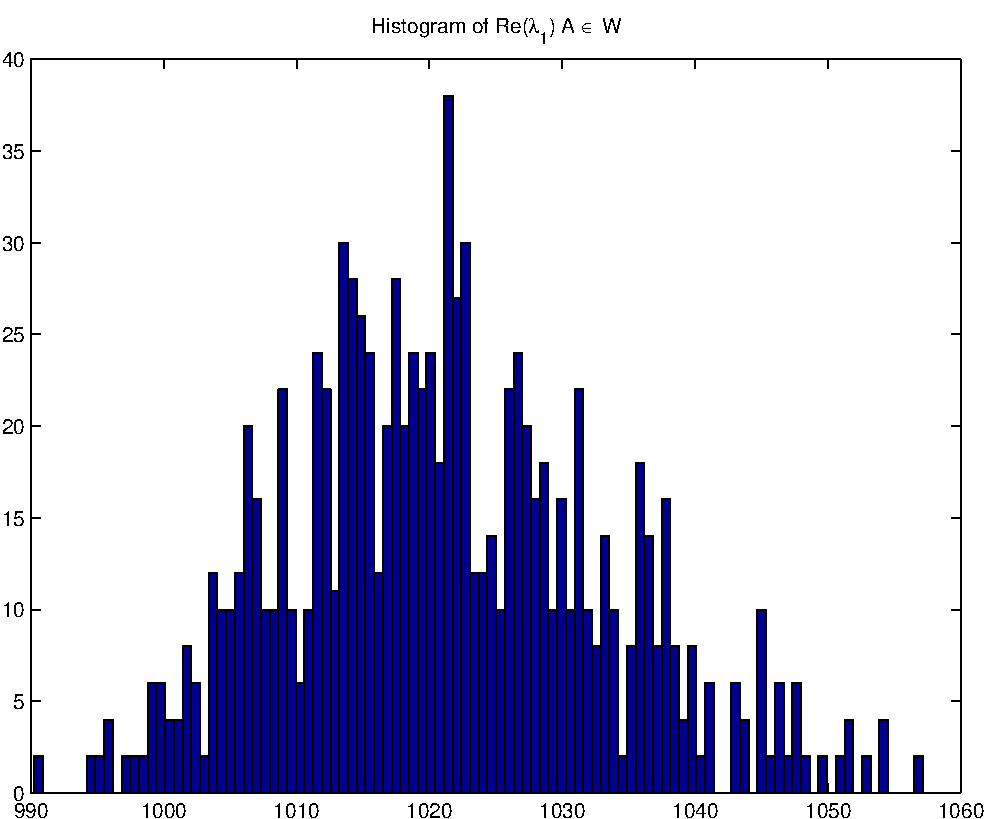
\includegraphics[width=10.0cm,height=10.0cm]{Re_TraceyWidom.pdf}

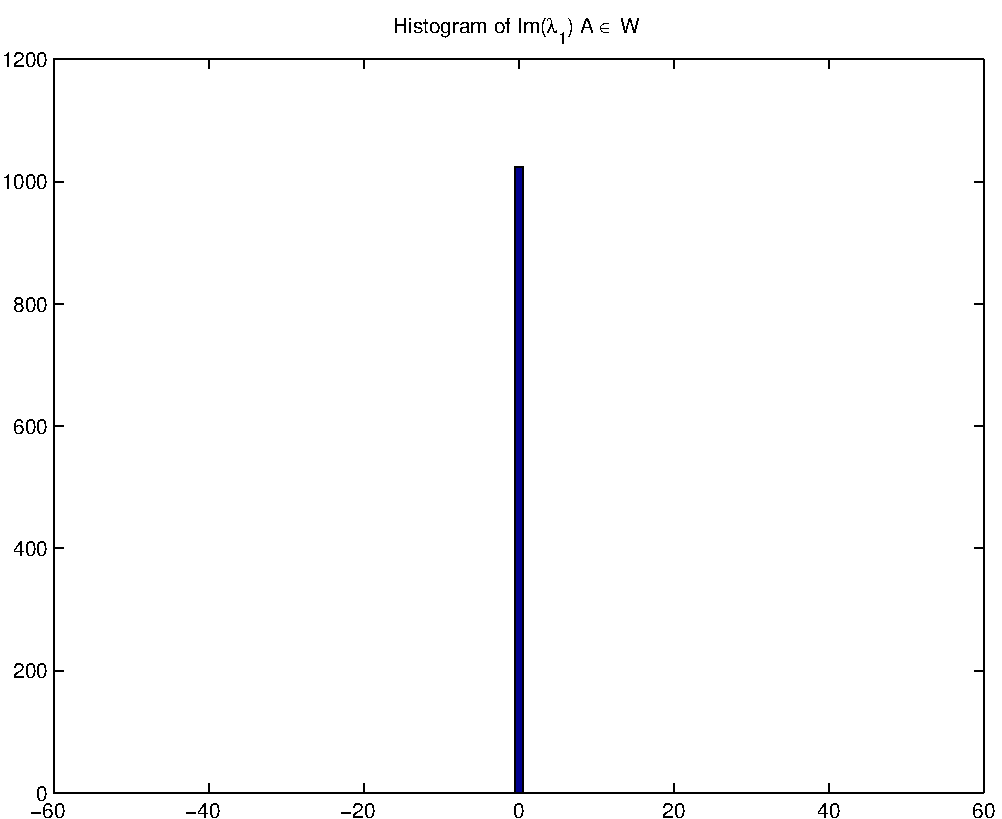
\includegraphics[width=10.0cm,height=10.0cm]{Im_TraceyWidom.pdf}

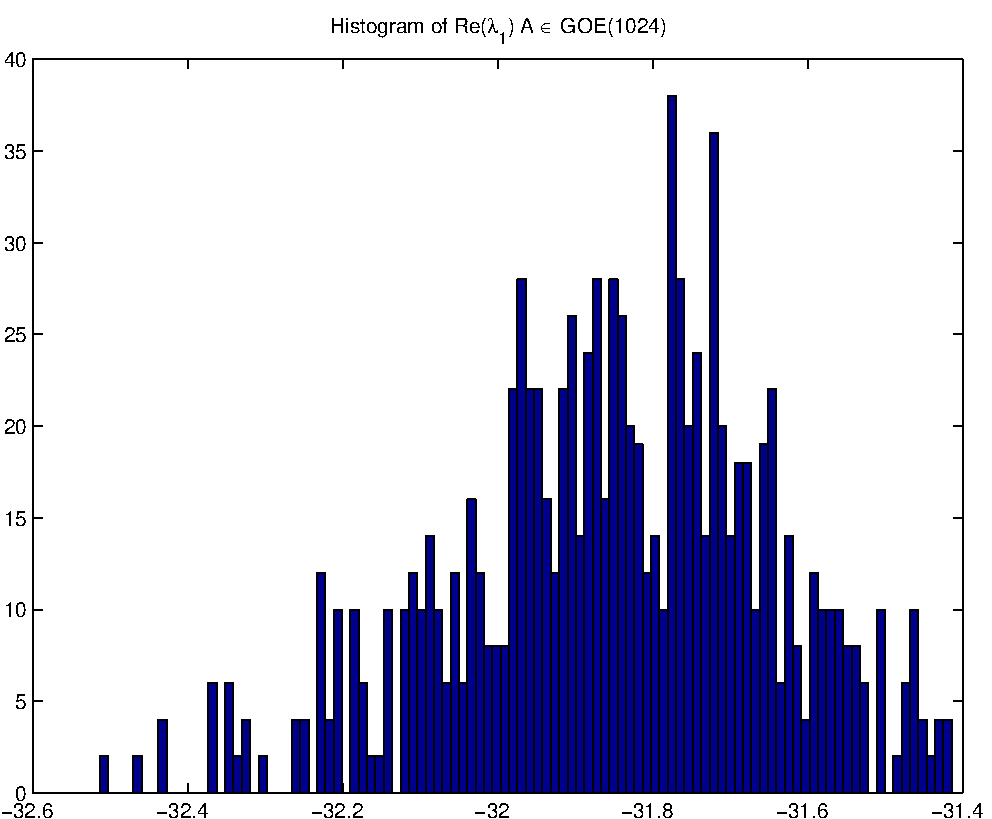
\includegraphics[width=10.0cm,height=10.0cm]{Re_Winger.pdf}

\includegraphics[width=10.0cm,height=10.0cm]{Im_Winger.pdf}

QueryPerformanceCounter  =  +4.997
\subsubsection{Approximate Winger Distribution}
\subsubsection{Verfy Winger Law.}
Let $M_n = [X_{ij} ]$ a symmetric n x n matrix with Random entries such that $X_{i,j} = X_{j,i}$, 		  and $X_{i,j}$ are iid $orall i < j,$ and $Xjj$ are iid $orall j  :  ; E[X^2_{ij} ] = 1, & E[X_{ij}] = 0$ 		  and that all moments exists for each of the entries.  		  The eigenvector of this random matrix; $ lambda_1 leq ... leq lambda_n$ depends continuously on $Mn$.
Dimension $n = +512$

\includegraphics[width=10.0cm,height=10.0cm]{Re_lambda_n.pdf}

\includegraphics[width=10.0cm,height=10.0cm]{Im_lambda_n.pdf}

QueryPerformanceCounter  =  +2.530
\subsubsection{Matrix Exponential }
$SPD Matrix = \left(
\begin{array}{
cccccccc}
+10.539 & -0.499 & -0.010 & +0.368 & +0.465 & -0.492 & -0.126 & +0.437 \\
-0.499 & +7.286 & +0.365 & -0.481 & -0.337 & -0.466 & +0.279 & +0.056 \\
-0.010 & +0.365 & +6.705 & -0.205 & +0.467 & +0.131 & +0.077 & -0.089 \\
+0.368 & -0.481 & -0.205 & +6.496 & -0.402 & -0.209 & +0.043 & -0.041 \\
+0.465 & -0.337 & +0.467 & -0.402 & +4.578 & +0.272 & +0.289 & -0.285 \\
-0.492 & -0.466 & +0.131 & -0.209 & +0.272 & +8.181 & +0.343 & -0.244 \\
-0.126 & +0.279 & +0.077 & +0.043 & +0.289 & +0.343 & +5.938 & -0.212 \\
+0.437 & +0.056 & -0.089 & -0.041 & -0.285 & -0.244 & -0.212 & +9.691 \\
\end{array}
\right)$ \newline 

$SPD Eigs = \left(
\begin{array}{
cccccccc}
(+10.93611,+0.00000) & (+9.60778,+0.00000) & (+4.23666,+0.00000) & (+8.36911,+0.00000) & (+7.56229,+0.00000) & (+5.82791,+0.00000) & (+6.54198,+0.00000) & (+6.33139,+0.00000) \\
\end{array}
\right)$ \newline 

$exp(SPD) = \left(
\begin{array}{
cccccccc}
+47863.969 & -6460.093 & -1078.770 & +4706.958 & +2535.224 & -8475.398 & -2406.368 & +12977.552 \\
-6460.093 & +2780.574 & +516.920 & -1069.918 & -548.083 & -109.707 & +386.466 & -807.216 \\
-1078.770 & +516.920 & +1015.281 & -385.755 & +176.069 & +458.541 & +212.284 & -859.022 \\
+4706.958 & -1069.918 & -385.755 & +1267.210 & +111.181 & -1018.272 & -287.809 & +1036.628 \\
+2535.224 & -548.083 & +176.069 & +111.181 & +413.265 & +135.193 & +45.490 & -502.411 \\
-8475.398 & -109.707 & +458.541 & -1018.272 & +135.193 & +5613.026 & +968.003 & -4270.737 \\
-2406.368 & +386.466 & +212.284 & -287.809 & +45.490 & +968.003 & +632.432 & -1645.725 \\
+12977.552 & -807.216 & -859.022 & +1036.628 & -502.411 & -4270.737 & -1645.725 & +19362.944 \\
\end{array}
\right)$ \newline 

$exp(SPD) eigs = \left(
\begin{array}{
cccccccc}
(+56168.17045,+0.00000) & (+14880.07985,+0.00000) & (+4311.77579,+0.00000) & (+1924.25027,+0.00000) & (+69.17669,+0.00000) & (+339.64809,+0.00000) & (+693.66208,+0.00000) & (+561.93669,+0.00000) \\
\end{array}
\right)$ \newline 

$log(exp(SPD) eigs)  = \left(
\begin{array}{
cccccccc}
(+10.93611,+0.00000) & (+9.60778,+0.00000) & (+8.36911,+0.00000) & (+7.56229,+0.00000) & (+4.23666,+0.00000) & (+5.82791,+0.00000) & (+6.54198,+0.00000) & (+6.33139,+0.00000) \\
\end{array}
\right)$ \newline 

$exp(Id) = \left(
\begin{array}{
cccccccc}
+2.718 & +0.000 & +0.000 & +0.000 & +0.000 & +0.000 & +0.000 & +0.000 \\
+0.000 & +2.718 & +0.000 & +0.000 & +0.000 & +0.000 & +0.000 & +0.000 \\
+0.000 & +0.000 & +2.718 & +0.000 & +0.000 & +0.000 & +0.000 & +0.000 \\
+0.000 & +0.000 & +0.000 & +2.718 & +0.000 & +0.000 & +0.000 & +0.000 \\
+0.000 & +0.000 & +0.000 & +0.000 & +2.718 & +0.000 & +0.000 & +0.000 \\
+0.000 & +0.000 & +0.000 & +0.000 & +0.000 & +2.718 & +0.000 & +0.000 \\
+0.000 & +0.000 & +0.000 & +0.000 & +0.000 & +0.000 & +2.718 & +0.000 \\
+0.000 & +0.000 & +0.000 & +0.000 & +0.000 & +0.000 & +0.000 & +2.718 \\
\end{array}
\right)$ \newline 

$exp(Id) eigs = \left(
\begin{array}{
cccccccc}
(+2.71828,+0.00000) & (+2.71828,+0.00000) & (+2.71828,+0.00000) & (+2.71828,+0.00000) & (+2.71828,+0.00000) & (+2.71828,+0.00000) & (+2.71828,+0.00000) & (+2.71828,+0.00000) \\
\end{array}
\right)$ \newline 

$log(exp(Id) eigs)  = \left(
\begin{array}{
cccccccc}
(+1.00000,+0.00000) & (+1.00000,+0.00000) & (+1.00000,+0.00000) & (+1.00000,+0.00000) & (+1.00000,+0.00000) & (+1.00000,+0.00000) & (+1.00000,+0.00000) & (+1.00000,+0.00000) \\
\end{array}
\right)$ \newline 

For $n  \in  \dblz [16,128)$ we calculate  $|( SPD(n) Eigs - log(exp(SPD(n)) eigs)|_{l^2}$

$|( SPD(n) Eigs - log(exp(SPD(n)) eigs)|_{l^2} = \left(
\begin{array}{
cccccccccccccccccccccccccccccccccccccccccccccccccccccccccccccccccccccccccccccccccccccccccccccccccccccccccccccccc}
(+5.36543,+0.00000) & (+5.36543,+0.00000) & (+5.36543,+0.00000) & (+5.36543,+0.00000) & (+5.36543,+0.00000) & (+5.36543,+0.00000) & (+5.36543,+0.00000) & (+5.36543,+0.00000) & (+5.36543,+0.00000) & (+5.36543,+0.00000) & (+5.36543,+0.00000) & (+5.36543,+0.00000) & (+5.36543,+0.00000) & (+5.36543,+0.00000) & (+5.36543,+0.00000) & (+5.36543,+0.00000) & (+5.36543,+0.00000) & (+5.36543,+0.00000) & (+5.36543,+0.00000) & (+5.36543,+0.00000) & (+5.36543,+0.00000) & (+5.36543,+0.00000) & (+5.36543,+0.00000) & (+5.36543,+0.00000) & (+5.36543,+0.00000) & (+5.36543,+0.00000) & (+5.36543,+0.00000) & (+5.36543,+0.00000) & (+5.36543,+0.00000) & (+5.36543,+0.00000) & (+5.36543,+0.00000) & (+5.36543,+0.00000) & (+5.36543,+0.00000) & (+5.36543,+0.00000) & (+5.36543,+0.00000) & (+5.36543,+0.00000) & (+5.36543,+0.00000) & (+5.36543,+0.00000) & (+5.36543,+0.00000) & (+5.36543,+0.00000) & (+5.36543,+0.00000) & (+5.36543,+0.00000) & (+5.36543,+0.00000) & (+5.36543,+0.00000) & (+5.36543,+0.00000) & (+5.36543,+0.00000) & (+5.36543,+0.00000) & (+5.36543,+0.00000) & (-2.44429,+0.00000) & (-2.23416,+0.00000) & (-2.12272,+0.00000) & (-1.68408,+0.00000) & (-1.46701,+0.00000) & (-1.42424,+0.00000) & (-1.19344,+0.00000) & (-1.00106,+0.00000) & (-0.79899,+0.00000) & (-1.32863,+0.00000) & (-0.03334,+0.00000) & (-0.18953,+0.00000) & (-0.70439,+0.00000) & (-0.53235,+0.00000) & (-0.34237,+0.00000) & (-2.07773,+0.00000) & (-0.59962,+0.00000) & (+11.22991,+0.00000) & (+10.41441,+0.00000) & (+10.46783,+0.00000) & (+9.90149,+0.00000) & (+9.80254,+0.00000) & (+9.43560,+0.00000) & (+9.32668,+0.00000) & (+8.69531,+0.00000) & (+8.60839,+0.00000) & (+8.50649,+0.00000) & (+8.10449,+0.00000) & (+8.00930,+0.00000) & (+7.80818,+0.00000) & (+7.62980,+0.00000) & (+7.49638,+0.00000) & (+7.27792,+0.00000) & (+7.03568,+0.00000) & (+6.93971,+0.00000) & (+6.68496,+0.00000) & (+6.65899,+0.00000) & (+6.18603,+0.00000) & (+6.36871,+0.00000) & (+6.35404,+0.00000) & (+5.89747,+0.00000) & (+5.79944,+0.00000) & (+5.64551,+0.00000) & (+5.48740,+0.00000) & (+5.39983,+0.00000) & (+5.21111,+0.00000) & (+5.10213,+0.00000) & (+5.05172,+0.00000) & (+4.79593,+0.00000) & (+4.74556,+0.00000) & (+4.57093,+0.00000) & (+4.35876,+0.00000) & (+3.88183,+0.00000) & (+4.00029,+0.00000) & (+3.64260,+0.00000) & (+3.45729,+0.00000) & (+3.28400,+0.00000) & (+3.19484,+0.00000) & (+3.07091,+0.00000) & (+2.94105,+0.00000) & (+2.86247,+0.00000) & (+2.58917,+0.00000) & (+2.40251,+0.00000) & (+2.34452,+0.00000) \\
\end{array}
\right)$ \newline 

QueryPerformanceCounter  =  +0.00949
The sample size generated for this run is 100000.

\newpage
uniform \begin{tabular}{|c|c|c|c|}  mean & variance & skewness & kurtosis \\  \hline
$\mu_1 = +0.50030$ & $\mu_2 = +0.08353$ & $\mu_3 = +0.00339$ & $\mu_4 =+1.80113$ \\
\end{tabular}

\includegraphics[width=5cm,height=5cm]{uniform.pdf}

cauchy \begin{tabular}{|c|c|c|c|}  mean & variance & skewness & kurtosis \\  \hline
$\mu_1 = +0.44288$ & $\mu_2 = +0.05341$ & $\mu_3 = +0.63935$ & $\mu_4 =+3.28094$ \\
\end{tabular}

\includegraphics[width=5cm,height=5cm]{cauchy.pdf}

exponential \begin{tabular}{|c|c|c|c|}  mean & variance & skewness & kurtosis \\  \hline
$\mu_1 = +1.99647$ & $\mu_2 = +3.99339$ & $\mu_3 = +2.03097$ & $\mu_4 =+9.30842$ \\
\end{tabular}

\includegraphics[width=5cm,height=5cm]{exponential.pdf}

\newpage
gamma \begin{tabular}{|c|c|c|c|}  mean & variance & skewness & kurtosis \\  \hline
$\mu_1 = +1.90062$ & $\mu_2 = +1.91694$ & $\mu_3 = +1.42724$ & $\mu_4 =+5.89964$ \\
\end{tabular}

\includegraphics[width=5cm,height=5cm]{gamma.pdf}

GIG \begin{tabular}{|c|c|c|c|}  mean & variance & skewness & kurtosis \\  \hline
$\mu_1 = +0.82337$ & $\mu_2 = +11.92158$ & $\mu_3 = +14.64211$ & $\mu_4 =+283.15426$ \\
\end{tabular}

\includegraphics[width=5cm,height=5cm]{GIG.pdf}

normal-box-muller \begin{tabular}{|c|c|c|c|}  mean & variance & skewness & kurtosis \\  \hline
$\mu_1 = -0.00036$ & $\mu_2 = +0.99804$ & $\mu_3 = -0.01010$ & $\mu_4 =+2.98492$ \\
\end{tabular}

\includegraphics[width=5cm,height=5cm]{normal-box-muller.pdf}

\newpage
normal-inverse-approximation \begin{tabular}{|c|c|c|c|}  mean & variance & skewness & kurtosis \\  \hline
$\mu_1 = +0.00230$ & $\mu_2 = +1.00486$ & $\mu_3 = +0.01163$ & $\mu_4 =+2.99254$ \\
\end{tabular}

\includegraphics[width=5cm,height=5cm]{normal-inverse-approximation.pdf}

pareto \begin{tabular}{|c|c|c|c|}  mean & variance & skewness & kurtosis \\  \hline
$\mu_1 = +3184578.26493$ & $\mu_2 = +888468246174112900.00000$ & $\mu_3 = +315.36997$ & $\mu_4 =+99629.09819$ \\
\end{tabular}

\includegraphics[width=5cm,height=5cm]{pareto.pdf}

poisson \begin{tabular}{|c|c|c|c|}  mean & variance & skewness & kurtosis \\  \hline
$\mu_1 = +1.10631$ & $\mu_2 = +0.13141$ & $\mu_3 = +3.89746$ & $\mu_4 =+20.78525$ \\
\end{tabular}

\includegraphics[width=5cm,height=5cm]{poisson.pdf}

\newpage
beta \begin{tabular}{|c|c|c|c|}  mean & variance & skewness & kurtosis \\  \hline
$\mu_1 = +0.33350$ & $\mu_2 = +0.12695$ & $\mu_3 = +0.68243$ & $\mu_4 =+1.91214$ \\
\end{tabular}

\includegraphics[width=5cm,height=5cm]{beta.pdf}

QueryPerformanceCounter  =  +11.12538
\subsubsection{Multiclass Support Vector Machine }
\begin{itemize}
\item Number or training points = 1024
\item Feature dimension = 3
\item Number or classes = 3
\end{itemize}
{The mean vectors of the 3 classes}

$\mu_1 = \left(
\begin{array}{
ccc}
+1.90000 & +0.10000 & +0.10000 \\
\end{array}
\right)$ \newline 

$\mu_2 = \left(
\begin{array}{
ccc}
+0.10000 & +1.90000 & +0.10000 \\
\end{array}
\right)$ \newline 

$\mu_3 = \left(
\begin{array}{
ccc}
+0.00000 & +0.00000 & +1.90000 \\
\end{array}
\right)$ \newline 

A random SPD covairance matrix is generated for each of the classes.\newline

$\rho_1 = \left(
\begin{array}{
ccc}
+2.247 & +0.100 & +0.436 \\
+0.100 & +2.066 & -0.384 \\
+0.436 & -0.384 & +3.158 \\
\end{array}
\right)$ \newline 

$\rho_2 = \left(
\begin{array}{
ccc}
+3.351 & -0.397 & -0.465 \\
-0.397 & +4.126 & +0.360 \\
-0.465 & +0.360 & +2.725 \\
\end{array}
\right)$ \newline 

$\rho_3 = \left(
\begin{array}{
ccc}
+4.227 & -0.138 & +0.064 \\
-0.138 & +4.324 & +0.491 \\
+0.064 & +0.491 & +2.971 \\
\end{array}
\right)$ \newline 

Verify $L_1$ condition number of covariance. The diagonal entries of the matrix have the form $(0.5 + U(0,1) )*dim(Dom(Cov))$
The lower-diagonal entries take the form $U(0,1) - 0.5$. 
The $L_1$ condition numbers are :
\begin{itemize}
\item +2.379
\item +2.230
\item +1.926
\end{itemize}
\includegraphics[width=10.0cm,height=10.0cm]{rv1_corr.pdf}

\includegraphics[width=10.0cm,height=10.0cm]{rv2_corr.pdf}

\includegraphics[width=10.0cm,height=10.0cm]{rv3_corr.pdf}

\includegraphics[width=10.0cm,height=10.0cm]{trainingPoints.pdf}

These are the SVM parameters - the RBF kernel is used\begin{itemize}
\item allOutlierFraction=0.05
\item mixingCoeff=0.3
\item smoThresh=1.0/10000.0
\item sigma=1
\end{itemize}
\includegraphics[width=10.0cm,height=10.0cm]{testPoints.pdf}

The marginal sample moments (mean var skew kurtosis) for training points.\newline
\begin{tabular}{ c |  c  c  c  c}
Feature & $\mu_1$ & $\mu_2$ & $\mu_3$ & $\mu_4$ \\
0 & +0.667 & +1.423 & +0.001& +2.271 \\
\hline
1 & +0.709 & +1.365 & +0.417& +2.581 \\
\hline
2 & +0.706 & +1.313 & +0.305& +2.416 \\
\hline
\end{tabular}
\newline
The marginal sample moments (mean var skew kurtosis) for test points.\newline
\begin{tabular}{ c | c  c  c  c}
Feature & $\mu_1$ & $\mu_2$ & $\mu_3$ & $\mu_4$ \\
0 & +0.677 & +1.306 & +0.132& +2.315\\
\hline
1 & +0.673 & +1.361 & +0.454& +2.624\\
\hline
2 & +0.726 & +1.222 & +0.299& +2.341\\
\hline
\end{tabular}\newline
\includegraphics[width=10.0cm,height=10.0cm]{classDiffs.pdf}

The error rate for this run is +0.160\newline
QueryPerformanceCounter  =  +6.249
\subsubsection{Semidefinite Programming SDPA}
QueryPerformanceCounter  =  +0.004
\end{document}
